%% 
%DIF LATEXDIFF DIFFERENCE FILE
%DIF DEL 1st-edition-7614/elsarticle-template-harv.tex    Tue Jan 28 08:06:02 2025
%DIF ADD cur-edition-10994/AgriMetSupport_qckInfill.tex   Thu Mar 13 13:46:38 2025
%% Copyright 2007-2019 Elsevier Ltd
%% 
%% This file is part of the 'Elsarticle Bundle'.
%% ---------------------------------------------
%% 
%% It may be distributed under the conditions of the LaTeX Project Public
%% License, either version 1.2 of this license or (at your option) any
%% later version.  The latest version of this license is in
%%    http://www.latex-project.org/lppl.txt
%% and version 1.2 or later is part of all distributions of LaTeX
%% version 1999/12/01 or later.
%% 
%% The list of all files belonging to the 'Elsarticle Bundle' is
%% given in the file `manifest.txt'.
%% 
%% Template article for Elsevier's document class `elsarticle'
%% with harvard style bibliographic references

% \documentclass[preprint,12pt,authoryear]{elsarticle}

%% Use the option review to obtain double line spacing
\documentclass[authoryear,preprint,review,12pt]{elsarticle}

%% Use the options 1p,twocolumn; 3p; 3p,twocolumn; 5p; or 5p,twocolumn
%% for a journal layout:
%% \documentclass[final,1p,times,authoryear]{elsarticle}
%% \documentclass[final,1p,times,twocolumn,authoryear]{elsarticle}
%% \documentclass[final,3p,times,authoryear]{elsarticle}
%% \documentclass[final,3p,times,twocolumn,authoryear]{elsarticle}
%% \documentclass[final,5p,times,authoryear]{elsarticle}
%% \documentclass[final,5p,times,twocolumn,authoryear]{elsarticle}

%% For including figures, graphicx.sty has been loaded in
%% elsarticle.cls. If you prefer to use the old commands
%% please give \usepackage{epsfig}

%% The amssymb package provides various useful mathematical symbols
\usepackage{amssymb}
%% The amsthm package provides extended theorem environments
%% \usepackage{amsthm}
\usepackage{amsmath}

%% Giuliano: add support for tif images
\usepackage{epstopdf}
\epstopdfDeclareGraphicsRule{.tif}{png}{.png}{convert #1 \OutputFile}
\AppendGraphicsExtensions{.tif}

%% The lineno packages adds line numbers. Start line numbering with
%% \begin{linenumbers}, end it with \end{linenumbers}. Or switch it on
%% for the whole article with \linenumbers.
\usepackage{lineno}
\usepackage[dvipsnames]{xcolor}
\usepackage[capitalize]{cleveref}
\usepackage[inline]{enumitem}
\usepackage{siunitx}
\usepackage{multirow}
\usepackage{xspace} % required by the \gci command
\usepackage{xparse} % required by the section redefinition
\usepackage{ifthen} % required by the section redefinition
\usepackage{booktabs} % For formal tables
%DIF 62a62-67
% --- Revision of 1st edition %DIF > 
%\usepackage[draft]{changes} %DIF > 
%\usepackage[final]{changes} %DIF > 
\usepackage{float} %DIF > 
\usepackage{subcaption} % Enables subfigures %DIF > 
\usepackage{xcolor}  % For highlighting %DIF > 
%DIF -------

%DIF 63d69
%DIF < 
%DIF -------
\newcommand{\note}[1]{\emph{\textcolor{red}{#1}}}
\newcommand{\update}[1]{\emph{\textcolor{blue}{#1}}}
\newcommand{\review}[1]{\emph{\textcolor{cyan}{#1}}}
\newcommand{\temp}[1]{\emph{\textcolor{gray}{#1}}}

\let\plainsection\section
\RenewDocumentCommand{\section}{s m o o}{
	\IfBooleanTF{#1}{
		% starred variant, unmodified
		\plainsection*{#2}
	}{
	    \IfNoValueTF{#3}{
	        % standard section
	        \plainsection{#2}
	    }{
	        \IfNoValueTF{#4}{
	            % only the assignee given
	            \plainsection{#2 (#3)}
	        }{
	        	\ifthenelse{
	        		\equal{#4}{todo}
	        	}{
	        		\plainsection{#2 (\textcolor{red}{#3 - TO DO})}
	        	}{}
	            \ifthenelse{
	            	\equal{#4}{wip}
	            }{
	            	\plainsection{#2 (\textcolor{red}{#3 - IN PROGRESS})}
	            }{}  
	        	\ifthenelse{
	        		\equal{#4}{update}
	        	}{
	        		\plainsection{#2 (\textcolor{blue}{#3 - UPDATE})}
	        	}{}
	        	\ifthenelse{
	        		\equal{#4}{review}
	        	}{
	        		\plainsection{#2 (\textcolor{cyan}{#3 - REVIEW})}
	        	}{}
	            \ifthenelse{
	            	\equal{#4}{done}
	            }{
	            	\plainsection{#2 (\textcolor{PineGreen}{#3 - READY})}
	            }{}
	        }
	    }
    }
}

\let\plainsubsection\subsection
\RenewDocumentCommand{\subsection}{s m o o}{
	\IfBooleanTF{#1}{
		% starred variant, unmodified
		\plainsubsection*{#2}
	}{
		\IfNoValueTF{#3}{
		    % standard section
		    \plainsubsection{#2}
		}{
		    \IfNoValueTF{#4}{
		        % only the assignee given
		        \plainsubsection{#2 (#3)}
		    }{
		    	\ifthenelse{
		    		\equal{#4}{todo}
		    	}{
		    		\plainsubsection{#2 (\textcolor{red}{#3 - TO DO})}
		    	}{}
		        \ifthenelse{
		        	\equal{#4}{wip}
		        }{
		        	\plainsubsection{#2 (\textcolor{red}{#3 - IN PROGRESS})}
		        }{}  
		    	\ifthenelse{
		    		\equal{#4}{update}
		    	}{
		    		\plainsubsection{#2 (\textcolor{blue}{#3 - UPDATE})}
		    	}{}
		     	\ifthenelse{
	        		\equal{#4}{review}
	        	}{
	        		\plainsubsection{#2 (\textcolor{cyan}{#3 - REVIEW})}
	        	}{}
		        \ifthenelse{
		        	\equal{#4}{done}
		        }{
		        	\plainsubsection{#2 (\textcolor{PineGreen}{#3 - READY})}
		        }{}
		    }
		}
	}
%DIF 155a160-177
} %DIF > 
 %DIF > 
\newcommand{\statusblock}[3]{ %DIF > 
    \ifthenelse{\equal{#2}{todo}} %DIF > 
        {\textcolor{red}{#1 (TO DO): #3}} %DIF > 
        {} %DIF > 
    \ifthenelse{\equal{#2}{wip}} %DIF > 
        {\textcolor{magenta}{#1 (IN PROGRESS): #3}} %DIF > 
        {} %DIF > 
    \ifthenelse{\equal{#2}{update}} %DIF > 
        {\textcolor{blue}{#1 (UPDATE): #3}} %DIF > 
        {} %DIF > 
    \ifthenelse{\equal{#2}{review}} %DIF > 
        {\textcolor{cyan}{#1 (REVIEW): #3}} %DIF > 
        {} %DIF > 
    \ifthenelse{\equal{#2}{done}} %DIF > 
        {\textcolor{PineGreen}{#1 (READY): #3}} %DIF > 
        {} %DIF > 
%DIF -------
}

%\newcommand{\gci}{\update{AgriMetSupport}\xspace}
% options are: Agriprog, WeatherProg-GCI, AgriSupport, AgriMetSupport, 

\journal{Computers and Electronics in Agriculture}

\bibliographystyle{model2-names}\biboptions{authoryear}
%DIF PREAMBLE EXTENSION ADDED BY LATEXDIFF
%DIF UNDERLINE PREAMBLE %DIF PREAMBLE
\RequirePackage[normalem]{ulem} %DIF PREAMBLE
\RequirePackage{color}\definecolor{RED}{rgb}{1,0,0}\definecolor{BLUE}{rgb}{0,0,1} %DIF PREAMBLE
\providecommand{\DIFadd}[1]{{\protect\color{blue}\uwave{#1}}} %DIF PREAMBLE
\providecommand{\DIFdel}[1]{{\protect\color{red}\sout{#1}}} %DIF PREAMBLE
%DIF SAFE PREAMBLE %DIF PREAMBLE
\providecommand{\DIFaddbegin}{} %DIF PREAMBLE
\providecommand{\DIFaddend}{} %DIF PREAMBLE
\providecommand{\DIFdelbegin}{} %DIF PREAMBLE
\providecommand{\DIFdelend}{} %DIF PREAMBLE
\providecommand{\DIFmodbegin}{} %DIF PREAMBLE
\providecommand{\DIFmodend}{} %DIF PREAMBLE
%DIF FLOATSAFE PREAMBLE %DIF PREAMBLE
\providecommand{\DIFaddFL}[1]{\DIFadd{#1}} %DIF PREAMBLE
\providecommand{\DIFdelFL}[1]{\DIFdel{#1}} %DIF PREAMBLE
\providecommand{\DIFaddbeginFL}{} %DIF PREAMBLE
\providecommand{\DIFaddendFL}{} %DIF PREAMBLE
\providecommand{\DIFdelbeginFL}{} %DIF PREAMBLE
\providecommand{\DIFdelendFL}{} %DIF PREAMBLE
%DIF AMSMATHULEM PREAMBLE %DIF PREAMBLE
\makeatletter %DIF PREAMBLE
\let\sout@orig\sout %DIF PREAMBLE
\renewcommand{\sout}[1]{\ifmmode\text{\sout@orig{\ensuremath{#1}}}\else\sout@orig{#1}\fi} %DIF PREAMBLE
\makeatother %DIF PREAMBLE
%DIF COLORLISTINGS PREAMBLE %DIF PREAMBLE
\RequirePackage{listings} %DIF PREAMBLE
\RequirePackage{color} %DIF PREAMBLE
\lstdefinelanguage{DIFcode}{ %DIF PREAMBLE
%DIF DIFCODE_UNDERLINE %DIF PREAMBLE
  moredelim=[il][\color{red}\sout]{\%DIF\ <\ }, %DIF PREAMBLE
  moredelim=[il][\color{blue}\uwave]{\%DIF\ >\ } %DIF PREAMBLE
} %DIF PREAMBLE
\lstdefinestyle{DIFverbatimstyle}{ %DIF PREAMBLE
	language=DIFcode, %DIF PREAMBLE
	basicstyle=\ttfamily, %DIF PREAMBLE
	columns=fullflexible, %DIF PREAMBLE
	keepspaces=true %DIF PREAMBLE
} %DIF PREAMBLE
\lstnewenvironment{DIFverbatim}{\lstset{style=DIFverbatimstyle}}{} %DIF PREAMBLE
\lstnewenvironment{DIFverbatim*}{\lstset{style=DIFverbatimstyle,showspaces=true}}{} %DIF PREAMBLE
\lstset{extendedchars=\true,inputencoding=utf8}

%DIF END PREAMBLE EXTENSION ADDED BY LATEXDIFF

\begin{document}

\begin{frontmatter}

%% Title, authors and addresses

%% use the tnoteref command within \title for footnotes;
%% use the tnotetext command for theassociated footnote;
%% use the fnref command within \author or \address for footnotes;
%% use the fntext command for theassociated footnote;
%% use the corref command within \author for corresponding author footnotes;
%% use the cortext command for theassociated footnote;
%% use the ead command for the email address,
%% and the form \ead[url] for the home page:
%% \title{Title\tnoteref{label1}}
%% \tnotetext[label1]{}
%% \author{Name\corref{cor1}\fnref{label2}}
%% \ead{email address}
%% \ead[url]{home page}
%% \fntext[label2]{}
%% \cortext[cor1]{}
%% \address{Address\fnref{label3}}
%% \fntext[label3]{}

%\title{weatherprog N1 publishing quality-controlled data from heterogeneous stations}
%\title{A cyber-physical infrastructure for agricultural meteorology and planning}
%\title{A platform for agricultural meteorology management \note{and planning (need more in the text)}: AgriMetSupport }
%\title{Agricultural meteorology management \note{and planning (develop it in the text)}: the AgriMetSupport platform }
%\title{A fully integrated platform for agricultural meteorology management and planning: the AgriMetSupport at work \note{to create certified data with no gaps} }
%\title{ Qualified data production for agricultural meteorology management and planning\review{: A case study using the AgriMetSupport infrastructure} }
%\title{ Qualified data production for agricultural meteorology management and planning: A case study using an interoperable cyber-physical system }
\title{Enhancing agricultural meteorology: qualified data production through an interoperable cyber-physical system}

%% use optional labels to link authors explicitly to addresses:
%% \author[label1,label2]{}
%% \address[label1]{}
%% \address[label2]{}

%\author{}
\author[dia,crisp]{Giuliano Langella\corref{cor}}
\address[dia]{Department of Agriculture, University of Naples Federico II, Via Università 100, 80055 Portici, NA, Italy}
\address[crisp]{Interdepartmental Research Centre on Earth Critical Zone, University of Naples Federico II, Via Università 100, 80055 Portici, NA, Italy}
\cortext[cor]{Corresponding author}
\ead{glangella@unina.it}

\date{May 2024}

\begin{abstract}
% Computers & Electronics in Agriculture: no longer than 400 words.
%Key Steps to Plan Writing an Abstract [A]
% 1. Introduction—what is the topic?
% 2. Statement of purpose?
% 3. Summarize why have other studies not tackled similar research questions?
% 4. How has the research question been tackled?
% 5. How was the research done?
% 6. What is the key impact of the research?
%
%The goal of writing an abstract is to communicate [B]:
% 1. What was done? 
% 2. Why was it done? 
% 3. How was it done? 
% 4. What was found? 
% 5. What is the significance of the findings?
%
% I follow the suggestion given in [B] to write the following abstract.
An interoperable \DIFdelbegin \DIFdel{cyber-physical system }\DIFdelend \DIFaddbegin \DIFadd{and geospatial Cyber-Physical System (CPS) }\DIFaddend -- called \DIFdelbegin \DIFdel{AgriMetSupport }\DIFdelend \DIFaddbegin \DIFadd{Agri\-Met\-Support }\DIFaddend -- was implemented to manage sensor networks, weather stations, agrometeorological data, and services that can be developed sequentially (e.g., models enabling territorial and integrated risk management).
Such a system could become crucial to support anyone responsible for establishing and maintaining an advanced sensor network, including territorial bodies, researchers, data analysts, and other stakeholders such as consortia of farmers, and those providing point and gridded sensor data support within research and development projects.
In the context of agrometeorological networks, this task is becoming increasingly difficult because it is required to deal with complex operations carried out using agrometeorological data such as data storage, quality check, missing data management, build continuous raster maps by means of geospatial modelling, data sharing with stakeholders and so forth.
In addition, responsible entities should implement these actions by pursuing complimentary objectives such as the adoption of standardized, scientifically-sound and perhaps shared procedures among federated territories.
\DIFdelbegin \DIFdel{AgriMetSupport }\DIFdelend \DIFaddbegin \DIFadd{Agri\-Met\-Support }\DIFaddend is made by physical, software and modular components which are all specifically designed to build an operative cyber-physical system supporting responsable entities in their management and planning tasks, but also any other stakeholder dealing with the production or the consumption of either sensor data or any kind of service based on these data.
The fundamental aim of the work proposed in this paper is to validate the production of qualified and certified data using well-tuned procedures available along with \DIFdelbegin \DIFdel{AgriMetSupport}\DIFdelend \DIFaddbegin \DIFadd{Agri\-Met\-Support}\DIFaddend .
The main finding is that such a cyber-physical structure can be spread to distinct territories (or distinct networks within the same territory) or can be used as the centralised system to manage federated monitoring networks.
It can ease the management of sensor networks by responsible entities while leaving complex issues to researchers or domain experts.
\end{abstract}

\begin{keyword}
%% keywords here, in the form: keyword \sep keyword
agricultural meteorology \sep cyber-physical system \sep validation of quality control \sep gap-filling procedure \sep digital and precision agriculture
%% PACS codes here, in the form: \PACS code \sep code

%% MSC codes here, in the form: \MSC code \sep code
%% or \MSC[2008] code \sep code (2000 is the default)
\end{keyword}

% HIGHLIGHTS
% 1) territorial bodies need advanced approaches to manage agro-meteorological data
% 2) the proposed cyber-physical system is made by both physical objects and advanced logics
% 3) an advanced logic of qualified and certified data production is validated
% 4) the proposed system simplifies any step from point-based measurements to digital climatic grids
% 5) the proposed system is in production in Campania Region and can be applied and scaled elsewhere

% HIGHLIGHTS (2024-05-18)
%	•	Innovative framework: development of AgriMetSupport, a modular and interoperable Geospatial Cyber-Infrastructure (GCI) tailored for sensor networks.
%	•	Core engine: Implementation of WeatherProg, the core engine, which automates data collection, validation, and geospatial prediction from diverse agrometeorological sensors.
%	•	Qualified data production: introduction of robust procedures for data quality control and gap-filling, ensuring high accuracy and reliability of agrometeorological data.
%	•	Real-world application: successful application and validation of AgriMetSupport in the Campania Region, demonstrating its effectiveness in real-world agricultural management.
%	•	Granularity and flexibility: demonstration of the system’s scalability, granularity and flexibility to adapt to various network configurations and stakeholder needs across different territories.

% HIGHLIGHTS (2024-31-05) - After Editor comments
% 1.	AgriMetSupport: a modular cyber infrastructure for sensor networks management
% 2.	WeatherProg automates data collection, validation, and prediction from sensors
% 3.	Robust control and gap-filling ensure accurate, reliable IoT data
% 4.	AgriMetSupport validated in Campania, proving effective in agriculture management
% 5.	System’s scalability and flexibility adapt to various networks and stakeholder needs

\end{frontmatter}

%\tableofcontents

\linenumbers

\section{Introduction}

%journal: Computers and Electronics in Agriculture
% https://www.journals.elsevier.com/computers-and-electronics-in-agriculture

% ==== Big Picture ====
%Include the big picture: The Earth Critical Zone requires that models such as SPA and pest models have quality checked data.
%\begin{itemize} 
%    \item Problem statement
%    \item Related work
%    \item Objectives
%\end{itemize}

% ==== Earth Critical Zone ====
%It is a living, breathing, constantly evolving boundary layer where rock, soil, water, air, and living organisms interact. These complex interactions regulate the natural habitat and determine the availability of life-sustaining resources, including our food production and water quality.
%The Critical Zone (CZ) is the support system for all terrestrial ecosystems, extending from unweathered rock to the top of any vegetation canopy. In the CZ, physical, biological, geological and hydrological processes interact at multiple temporal and spatial scales.
%Earth's critical zone is the “heterogeneous, near surface environment in which complex interactions involving rock, soil, water, air, and living organisms regulate the natural habitat and determine the availability of life-sustaining resources”
\DIFaddbegin \statusblock{}{wip}{NOTES: (1) remove any reference to GCI and use CPS in the whole paper; (2) check that at crucial locations in the manuscript I highlight the distinct feature of \textit{geospatial} for my CPS.}

\DIFaddend Climate controls the Earth's Critical Zone (ECZ) in combination with other physical, biological and geological processes.
The ECZ is a heterogeneous system extending from the top of the vegetation canopy to the bottom of unweathered rocks, regulates the availability of resources and modulates the production of ecosystem services such as the filtration and quality of water, and the production of food and fibre.

% ==== Agricultural Meteorology ====
% LINKS:
%   https://books.google.it/books?id=vdFBDwAAQBAJ&pg=PA22&lpg=PA22&dq=importance+of+agrometeo+measurements&source=bl&ots=CmcFAArYyq&sig=ACfU3U1TMqCpGqAv7VZjSz1M_IgPKv1--w&hl=it&sa=X&ved=2ahUKEwjPs_Tdg_vgAhXQ4KQKHYM3B4AQ6AEwAHoECAkQAQ#v=onepage&q=importance%20of%20agrometeo%20measurements&f=false
%   http://www.agrometeorology.org/files-folder/repository/gamp1.pdf
%   https://en.wikibooks.org/wiki/Introductory_Agrometeorology/Introduction
%   http://www.agrilearner.com/agrometeorology-needs-scope/
%   http://www.agriinfo.in/default.aspx?page=topic&superid=1&topicid=377

%Weather: Physical state of the atmosphere at a given place and given time. Eg. Cloudy day
%Climate: Long term regime of atmospheric variables of a given place or area. Eg. Cold season
%and considered as basic input or resources in agricultural planning, every plant process related with growth development and yield of a crop is affected by weather.

Weather and climate are the most important dynamic components of the ECZ determining the physical \DIFdelbegin \DIFdel{condition }\DIFdelend \DIFaddbegin \DIFadd{conditions }\DIFaddend in which animals and plants are grown.
Weather is the physical state of the atmosphere at any spatiotemporal coordinate, while climate represents an aggregation of atmospheric variables mostly over time (e.g. seasonal extremes) but also in the spatial domain (e.g. regional extremes).
Agricultural meteorology is concerned with the monitoring of weather and the characterisation of the meteorological, hydrological and pedological factors that have a direct effect on agriculture and the production of crops and livestocks.
% http://www.agriinfo.in/default.aspx?page=topic&superid=1&topicid=377
Agricultural meteorology is deemed important considering the large amount of ground stations available worldwide to monitor the behaviour of weather elements, notwithstanding, for instance, the huge amounts of air-borne proxy products coming from massive satellite monitoring.
Indeed, amongst others, it helps: 
    \begin{enumerate*}
        \item understanding the realisation of several crop parameters such as the growing season and the harvesting time;  \citep{Hoogenboom:agrometeo-swat:2000,Chou2019,Madhukar2021,Richmond2022};
        \item managing crops by means of various farm operations such as fertilisers application and irrigation scheduling \citep{Cammarano2021,Chen2020};
        \item assessing the suitability of specific crops both in space for instance by means of agroclimatic zoning and in time in particular according to climate change \citep{Rokochynskiy2020,Jiang2020};
        \item crop and livestock monitoring and modelling \citep{Vogel2021,Zhang2022};
        \item understanding the spatial distribution of soil types and soil properties since climate is one of the soil forming factors recognized in both CLORPT \citep{jenny:clorpt:1941} and SCORPAN \citep{McBratney:scorpan:2003} models;
        \item forecasting plant pests and diseases \citep{IPM_decisions}.
    \end{enumerate*}

\subsection{Related work}
There is an increasing demand for the production, in digital format, of weather and climatic data of good quality within the earth critical zone both 
    for practical applications (e.g. the need to know climatic patterns in a farm to improve the management)
    and
    for research and development, in particular to simulate the soil-plant-atmosphere system \citep{Hoogenboom:agrometeo-swat:2000,Jones:swat:2003,Seneviratne:swat:2010} % \citep{Langella:rainann:2010}
    and the risk of pests \citep{Orlandini:plasmopara:2008,Rossi:vitenet:2014}.
    % \citep{Terribile:dssvitis:2017}
The demand is particularly burdensome considering the requirement to handle climatic data both at finer temporal scale and in a continuous spatial domain.
It means that daily (e.g. in the soil hydrological modelling) or even hourly records (e.g. in the phytopathologic risk modelling) measured at point gauges sparsely located in a territory must be transformed in three dimensional climatic data cubes (Longitude, Latitude, Time) by means of statistically sound geospatial procedures.
% (there is a gap between the major of scientific modelling approaches that requires digital climate maps and the gauged measurements).
There exist few approaches implementing and deploying automatic spatial inference engines of this kind based on point agrometeorological data at the daily or even at the hourly time step.
One example working in USA using already checked daily data, is given by the expert-based model called PRISM developed by  \cite{Daly08_PRISM_USA}. %\note{(search for other REFs? may be sufficient!)}

% ==== Aim ====
%Support systems to agrometeorological practices and services comprise data (so quantification), research, training/education/extension and policy environments. Especially in industrialized countries mathematical models are increasingly used in operational agricultural meteorology, in conjunction with Geographic Information Systems (GISs) to provide inputs to Decision Support Systems (DSSs).
Especially in more developed countries, mathematical models are increasingly used in agriculture in conjunction with Geographic Information Systems (GISs), also via web in the form of WebGIS, to provide inputs to Decision Support Systems (DSSs), possibly via web in the form of Web Based geoSpatial Decision Support Systems (WB-SDSS).
Examples of WB-SDSS can be found 
for heavy metal pollution management in soils \citep{Wang:wbsdss:2017}, 
for livestock manure management \citep{Acutis:wbsdss:2014}, 
for locust prevention and control \citep{Yao:wbsdss:2017}, 
for optimized crop irrigation \citep{Giusti:wbsdss:2015}, 
for land management and soil conservation \citep{Terribile:LandSupport:2024}, 
for early warning systems in areas of weather and climate \citep{Bopape_2019},
and so forth.
%\review{ include also examples of possibile similar GCIs such as \citep{Bopape_2019}...; hydrometeorological;  }
There exist a huge production of DSS tools on quite every issue related to the agricultural and forestry systems.
%\note{what is missing? a GCI on agrometerological data to facilitate the assembly of tools to support decision process in issues related to agriculture and forestry.  }
\DIFdelbegin \DIFdel{To authors' knowledge, there is a gap in literature concerning Geospatial Cyber-Infrastructures (GCIs) fully dedicated to agriculture meteorology, both to implement a stand-alone agrometeorological platform and to facilitate the assembly of tools to support the decision process in issues related to the earth critical zone with particular reference to agriculture and forestry. 
Results obtained on scopus.com (May 2024) reveals that 386 documents (articles, reviews and books) were published on cyber infrastructures applied in (agro-)meteorology, while none of them were relevant to the peculiar scope of this work.
}\DIFdelend \DIFaddbegin \statusblock{}{wip}{To author knowledge, there is a gap in literature concerning Geospatial Cyber-Infrastructures (GCIs) or Cyber-Physical Systems (CPSs) fully dedicated to agriculture meteorology, both to implement a stand-alone agrometeorological platform and to facilitate the assembly of tools to support the decision process in issues related to the earth critical zone with particular reference to agriculture and forestry. 
Results obtained on scopus.com (Jan 2025) reveals that \textbf{CHECK}(386) documents (articles, reviews and books) were published on cyber infrastructures applied in (agro-)meteorology, while none of them were relevant to the peculiar scope of this work.
A search with "Cyber Physical System Agriculture Meteorology" returned \textbf{CHECK}(few documents) such as \cite{sarkar24CPS}.
It appears that existing CPSs primarily focus on single-location environments, whereas Agri\-Met\-Support is designed to address the complexities of heterogeneous landscapes and diverse territories by incorporating sensor networks. 
This unique feature is advantageous since crucial operations such as the quality check and data gap infilling at each location leverage information from other locations.\\
Highlight pros and cons.\\
Pros:
\begin{itemize}
    \item management of sensor networks; 
    \item WeatherProg modules dedicated to quality control, gap infilling, spatial interpolation and gridded datacubes;
    \item AMS is a geospatial CPS differently from other CPSs (highlight its ability to process geospatial data in real time; differentiate it from generic CPS that might not handle spatial information (at least in AGRI- domain); strengthen its connection to agrometeorology, where spatial data is key)
\end{itemize}
Cons:
\begin{itemize}
    \item Agri\-Met\-Support by design misses the actuation modules even though it provides APIs (Application Programming Interfaces) to data and modeling components to feed external services implementing actions;
    \item others?
\end{itemize}}

\DIFaddend % To authors' knowledge there is any work in literature dealing with GCI
% SCOPUS = "geospatial cyber infrastructure agrometeorology" ==> 0 results
% SCOPUS = "cyber infrastructure agrometeorology" ==> 0 results
% SCOPUS = "cyberinfrastructure meteorology" ==> 13 results, but not pertinent
% SCOPUS = "geospatial agrometeorology decision support" ==> 0 results
% SCOPUS,Dec-2022 = cyber AND infrastructure AND meteorology ==> 314 documents, see list of selected 25 documents in my private area on SCOPUS.

\subsection{Objectives}
% Research Problem:
Effective management and planning in agricultural meteorology require accurate, high-quality, and continuously updated data.
However, the increasing complexity of agrometeorological networks, coupled with the need for standardized and scientifically sound procedures, poses significant challenges for stakeholders responsible for these tasks.
To address these challenges, a comprehensive solution through the development of a modular and interoperable \DIFdelbegin \DIFdel{cyber-physical system, called AgriMetSupport, }\DIFdelend \DIFaddbegin \DIFadd{Cyber-Physical System (CPS) }\DIFaddend is proposed.

% Objectives:
To achieve this goal, the present study focuses on the following objectives:
\begin{enumerate}
    \item \DIFdelbegin \DIFdel{develop a }\DIFdelend \DIFaddbegin \DIFadd{Develop a }\statusblock{}{wip}{geospatial(AMS pros)}\DIFadd{, }\DIFaddend modular and interoperable \DIFdelbegin \DIFdel{cyber-physical system (}\DIFdelend \DIFaddbegin \DIFadd{CPS, called }\DIFaddend Agri\-Met\-Support\DIFdelbegin \DIFdel{) }\DIFdelend \DIFaddbegin \DIFadd{, }\DIFaddend that supports the  management\DIFaddbegin \DIFadd{, dissemination and use }\DIFaddend of agrometeorological data \DIFaddbegin \DIFadd{(\mbox{%DIFAUXCMD
\cref{sec:gci} }\hskip0pt%DIFAUXCMD
and \mbox{%DIFAUXCMD
\cref{sec:weatherprog}}\hskip0pt%DIFAUXCMD
)}\DIFaddend .
    \item \DIFdelbegin \DIFdel{tune }\DIFdelend \DIFaddbegin \DIFadd{Tune }\DIFaddend a fully automatic procedure %(or assisted if required) 
    to quality check and gap-fill measurements using standardised procedures \DIFaddbegin \DIFadd{(\mbox{%DIFAUXCMD
\cref{sec:qck+fill}}\hskip0pt%DIFAUXCMD
). }\DIFaddend %obtained from gauging stations.
    \item \DIFdelbegin \DIFdel{validate }\DIFdelend \DIFaddbegin \DIFadd{Demonstrate }\DIFaddend the system's \DIFdelbegin \DIFdel{ability to produce qualified, certified, and gap-filled data.
    }%DIFDELCMD < \item %%%
\item%DIFAUXCMD
\DIFdel{demonstrate the system's }\DIFdelend applicability and effectiveness in a real-world case study involving the Campania Region in Italy \DIFdelbegin \DIFdel{.
}\DIFdelend \DIFaddbegin \DIFadd{(\mbox{%DIFAUXCMD
\cref{sec:casestudy}}\hskip0pt%DIFAUXCMD
).
    }\item \DIFadd{Validate the system's ability to produce qualified, certified, and gap-filled data through perturbation (\mbox{%DIFAUXCMD
\cref{sec:QcheckValidation}}\hskip0pt%DIFAUXCMD
).
    }\item \statusblock{}{wip}{Estabilish that AgriMetSupport is valuable in research and science (\cref{sec:Valuability})\\
    (to answer \textbf{Q5R2}).
    NOTES: I have to highlight two distinct things:\\
     1) research: how AMS becomes useful, for instance to develop and validate models in agriculture, such as pest, soil, etc. I can provide the two examples at steps 6 and 9 of both \cref{Fig:WeatherProg} and \cref{Box01:WeatherProg_Operations}. Discuss how AgriMetSupport supports new research opportunities, such as monitoring microclimate dynamics, testing novel agronomic models, or evaluating extreme weather impacts.\\
     2) science: this is very difficult! I have to brainstorm about it\\
     FURTHER: Contributo alla ricerca: Devo prendere lo step 6 e/o 9 di WeatherProg e illustrare il vantaggio dal punto di vista della ricerca e scientifico nell’avere i moduli fondamentali di “aggiustamento” del dato (check + infill), applicati ad esempio nella messa a punto di un modello parassitario (e posso richiamare i due esempi prodotti negli step 6 e 9).
Contributo scientifico: il meccanismo di perturbazione e di validazione incrociata (NON CREDO DI AVERLO MAI CITATO NEL PAPER: POSSO PUNTARE SU QUESTO ASPETTO; IN REALTA’ LA VALIDAZIONE INCROCIATA È GIÀ IN ESSERE PER INFILL, MENTRE L’UNICO MODO PER TESTARE IL CONTROLLO DI QUALITÀ È INTRODURRE NOISE) può generare delle statistiche in termini di incertezza / errore che possono essere utilizzati sia per misurare la performance di AMS che per determinare la propagazione dell’incertezza e dell’errore nelle applicazioni e servizi a valle.
}
\DIFaddend \end{enumerate}

% agrimetsupport
%AgriMetSupport is a general technological framework, functioning as a WB-SDSS.
%This system can be fully tailored to the specific needs of an existent sensor networks, such as an grometeorological networks managed by local entrusted/responsible entities.
%In this context, "responsible entities" or "stakeholders" refer to local government agencies, researchers, consortia of farmers, and other similar entities involved in the management and use of agrometeorological data.
% weatherprog
%The proposed GCI is based on a software component, namely WeatherProg \citep{langella:weatherprog2014,langella:weatherprog2016}, which serves as the main engine of the information technology system.
%WeatherProg has the potential to be the basic engine of several geospatial-based services in agriculture, where both weather and climatic information is of paramount importance.
%It implements all tasks from gathering raw measurements from agrometeorological sensors to delivering digital climatic maps at different time steps (e.g., hourly, daily).

\DIFdelbegin \DIFdel{This study presents the design, implementation, and validation of AgriMetSupport, focusing on its modular components and the core engine, WeatherProg.
%DIF < The fundamental aim is to validate the production of qualified and certified data using well-tuned procedures available within AgriMetSupport.
The system can be fully tailored to the specific needs of existing sensor networks %DIF < , such as grometeorological networks
managed by local entrusted/responsible entities.
In this context, "responsible entities" or "stakeholders" refer to local government agencies, researchers, consortia of farmers, and other similar entities involved in the management and use of agrometeorological data.
The main finding is that such a cyber-physical structure can be spread to distinct territories (or distinct networks within the same territory) or used as a centralized system to manage federated monitoring networks.
It can ease the management of sensor networks by responsible entities while leaving complex issues to researchers or domain experts.
}%DIFDELCMD < 

%DIFDELCMD < %%%
%DIF <  Hypotheses:
%DIF < \note{1. AgriMetSupport can significantly improve the efficiency and accuracy of agrometeorological data management compared to existing systems, if any.
%DIF < 2. The system's modular architecture allows for flexible adaptation to different network configurations and stakeholder needs.
%DIF < 3. The validated data produced by AgriMetSupport will enhance decision-making processes in agricultural management and planning.}
%DIF < Together with the presentation of the general template WB-SDSS, the results of applying the AgriMetSupport GCI to a specific case study, that is in Campania Region (South of Italy), is shown with the specific focus of producing qualified and certified data.
%DIF < The task consists in tuning a fully automatic or assisted procedure to quality check and gap-fill the measurements carried out at gauged points.
%DIF < This is of particular relevance due to limitations and constraints (showed in \cref{sec:qcheck}) of the Campania Region agrometeorological network.
%DIFDELCMD < 

%DIFDELCMD < %%%
\DIFdel{The }\DIFdelend \DIFaddbegin \DIFadd{To this regard, the }\DIFaddend work is organized hierarchically, starting with general concepts and items and progressing to more detailed parts.
In section \ref{sec:gci} the overall \DIFdelbegin \DIFdel{geospatial cyber-infrastructure (AgriMetSupport) implementing the decision support system }\DIFdelend \DIFaddbegin \DIFadd{cyber-physical system (Agri\-Met\-Support) }\DIFaddend is described.
In section \ref{sec:weatherprog} the core engine (WeatherProg) processing the agrometeorological data is shown with emphasis on the main modules and their role in the infrastructure.
It is emphasised the high flexibility of the whole platform and the high granularity of its components.
Section \ref{sec:qck+fill} provides details about the data quality control and the gap-filling procedures, highlighting the operations required to produce data of good quality \DIFdelbegin \DIFdel{to be used in cascade in other 
applications}\DIFdelend \DIFaddbegin \statusblock{}{wip}{(REMOVE?)to be used in cascade in other applications}\DIFaddend .
The deployment of the \DIFdelbegin \DIFdel{AgriMetSupport GCI }\DIFdelend \DIFaddbegin \DIFadd{Agri\-Met\-Support CPS }\DIFaddend to a real case, namely in Campania Region\DIFdelbegin \DIFdel{(South of Italy)}\DIFdelend , is presented in section \ref{sec:casestudy}.
%DIF > This study presents the design, implementation, and validation of AgriMetSupport, focusing on its modular components and the core engine, WeatherProg.
%DIF > The fundamental aim is to validate the production of qualified and certified data using well-tuned procedures available within AgriMetSupport.
\DIFaddbegin \DIFadd{Indeed, the system can be fully tailored to the specific needs of existing sensor networks %DIF > , such as grometeorological networks
managed by local entrusted/responsible entities.
In this context, "responsible entities" or "stakeholders" refer to local government agencies, researchers, consortia of farmers, and other similar entities involved in the management and use of agrometeorological data.
}\statusblock{}{wip}{In \cref{sec:Valuability}, the value of the Agri-Met-Support geospatial CPS is demonstrated in both research applications and scientific advancements.}
\DIFaddend 

\DIFaddbegin \statusblock{}{wip}{REMOVE OR MOVE: The main finding is that such a cyber-physical system can be spread to distinct territories (or distinct networks within the same territory) or used as a centralized system to manage federated monitoring networks.
It can ease the management of sensor networks by responsible entities while leaving complex issues to researchers or domain experts.}

%DIF >  Hypotheses:
%DIF > \note{1. AgriMetSupport can significantly improve the efficiency and accuracy of agrometeorological data management compared to existing systems, if any.
%DIF > 2. The system's modular architecture allows for flexible adaptation to different network configurations and stakeholder needs.
%DIF > 3. The validated data produced by AgriMetSupport will enhance decision-making processes in agricultural management and planning.}
%DIF > Together with the presentation of the general template WB-SDSS, the results of applying the AgriMetSupport GCI to a specific case study, that is in Campania Region (South of Italy), is shown with the specific focus of producing qualified and certified data.
%DIF > The task consists in tuning a fully automatic or assisted procedure to quality check and gap-fill the measurements carried out at gauged points.
%DIF > This is of particular relevance due to limitations and constraints (showed in \cref{sec:qcheck}) of the Campania Region agrometeorological network.

\DIFaddend \section{\DIFdelbegin \DIFdel{The AgriMetSupport cyber-physical infrastructure}\DIFdelend \DIFaddbegin \DIFadd{Agri\-Met\-Support CPS}\DIFaddend } \label{sec:gci}
%Central to the design of an effective automated data-processing system is the database. The telecommunications subsystem database must hold:
%(a) Bulletins of incoming messages;
%(b) Locally generated observations;
%(c) Products for national dissemination;
%(d) Bulletins of locally generated observations for transmission on the GTS.
%The applications subsystem database must hold:
%(a) Reports derived from decoded bulletins;
%(b) Fields derived from decoded bulletins;
%(c) Products prepared through the processing of reports and fields.
%If possible, the database residing in each computer should be controlled by the same database
%management system (DBMS), which should be relatively simple so as to minimize computing overheads and facil- itate the speed of response of the overall data-processing system.

\DIFdelbegin \DIFdel{AgriMetSupport }\DIFdelend \DIFaddbegin \statusblock{}{wip}{ADD:\\
(1) emphasize AMS's geospatial component;\\
(2) define AMS as a "Geospatial CPS": make sure to clarify why this feature matters (e.g., AMS uses spatial interpolation, spatial-temporal modeling, or GIS-based decision support).
}

\DIFadd{Agri\-Met\-Support }\DIFaddend is designed to be a comprehensive framework for agrometereological monitoring and data management.
It can be effectively used for a wide range of purposes, from simple agrometeorogical monitoring to digital climatic maps production and agricultual and forestry modeling and application, including predictive pest modeling.
Clearly, different real-world applications have different requirements, which can be all accomodated by \DIFdelbegin \DIFdel{AgriMetSupport }\DIFdelend \DIFaddbegin \DIFadd{Agri\-Met\-Support }\DIFaddend thanks to its strongly modular architecture.
Components can be added or removed to a specific instance of \DIFdelbegin \DIFdel{AgriMetSupport }\DIFdelend \DIFaddbegin \DIFadd{Agri\-Met\-Support }\DIFaddend effortlessly without affecting other parts of the system, as well as modules of the core engine, namely WeatherProg, which can be selectively enabled or disabled.
This way, responsible entities can actually derive their own tailored instances from the general model of \DIFdelbegin \DIFdel{AgriMetSupport}\DIFdelend \DIFaddbegin \DIFadd{Agri\-Met\-Support}\DIFaddend .

The high-level architecture is illustrated in \cref{cyberPhysicalSystemFig}.
At the topmost level, \DIFdelbegin \DIFdel{AgriMetSupport }\DIFdelend \DIFaddbegin \DIFadd{Agri\-Met\-Support }\DIFaddend is constituted by central components responsible for storage\DIFdelbegin \DIFdel{(postgreSQL with postGIS extension) and }\DIFdelend \DIFaddbegin \DIFadd{, both in point and raster databases, and }\DIFaddend processing of data (\DIFdelbegin \DIFdel{e.g. }\DIFdelend \DIFaddbegin \DIFadd{i.e. }\DIFaddend WeatherProg).
Peripheral physical components are in charge of collecting data from the environment (i.e. sensors \DIFdelbegin \DIFdel{in }\DIFdelend \DIFaddbegin \DIFadd{and stations within }\DIFaddend the network) and peripheral software components deliver web services, such as \DIFdelbegin \DIFdel{web applications }\DIFdelend \DIFaddbegin \DIFadd{pest and IPM platforms or dashboards (e.g. }\DIFaddend enabling the agrometeorological data consulting by end-users\DIFdelbegin \DIFdel{.
}%DIFDELCMD < 

%DIFDELCMD < \begin{figure}
%DIFDELCMD < 	%%%
\DIFdelendFL \DIFaddbeginFL \DIFaddFL{).
}\begin{figure}[!t] %DIF >  [H] ensures the figure appears exactly here
	\DIFaddendFL \centering % trim=left bottom right top
	\DIFdelbeginFL %DIFDELCMD < 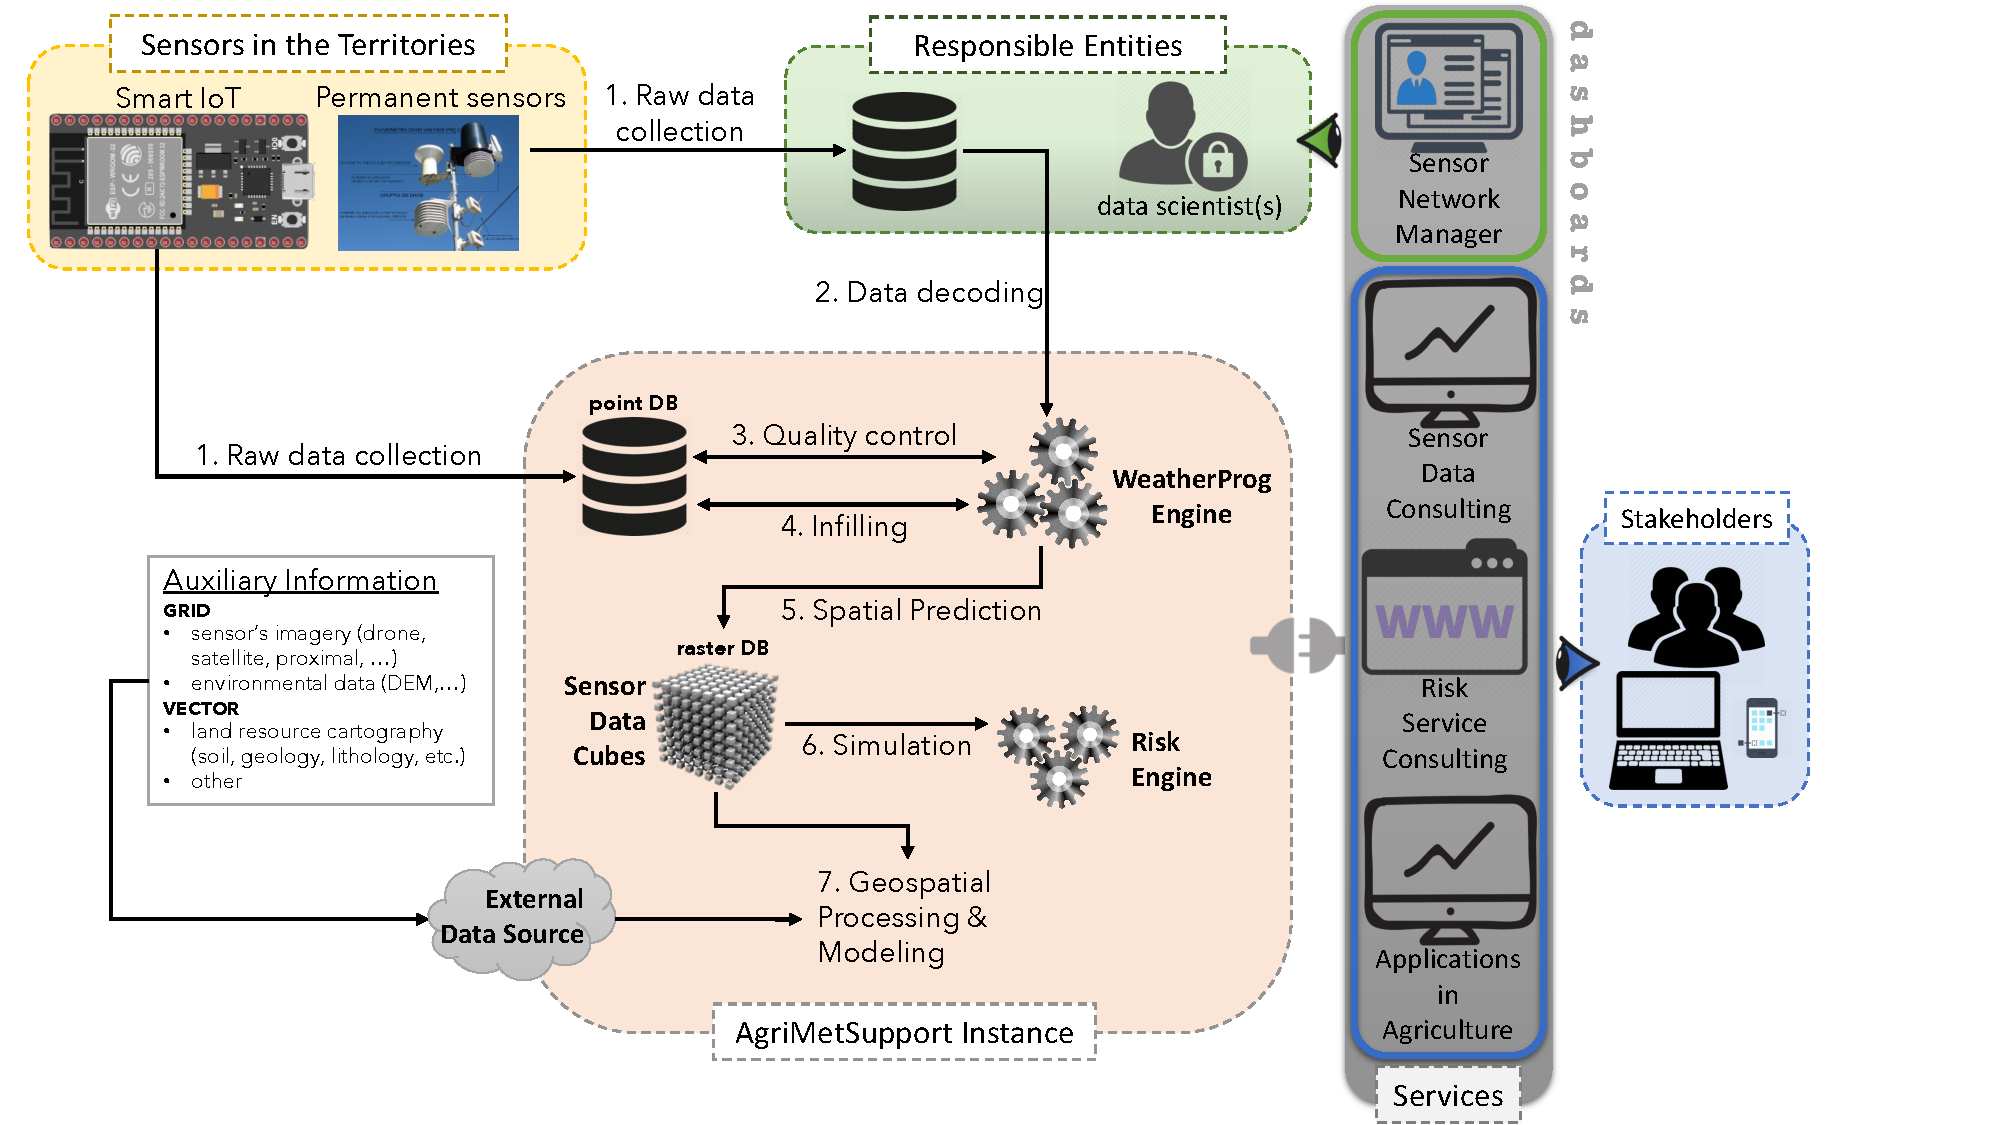
\includegraphics[angle=90,scale=.70,trim=1cm 2cm 8cm 2cm]{figures/AgriMetSupport-fig_v2.pdf}
%DIFDELCMD < 	%%%
\DIFdelendFL \DIFaddbeginFL 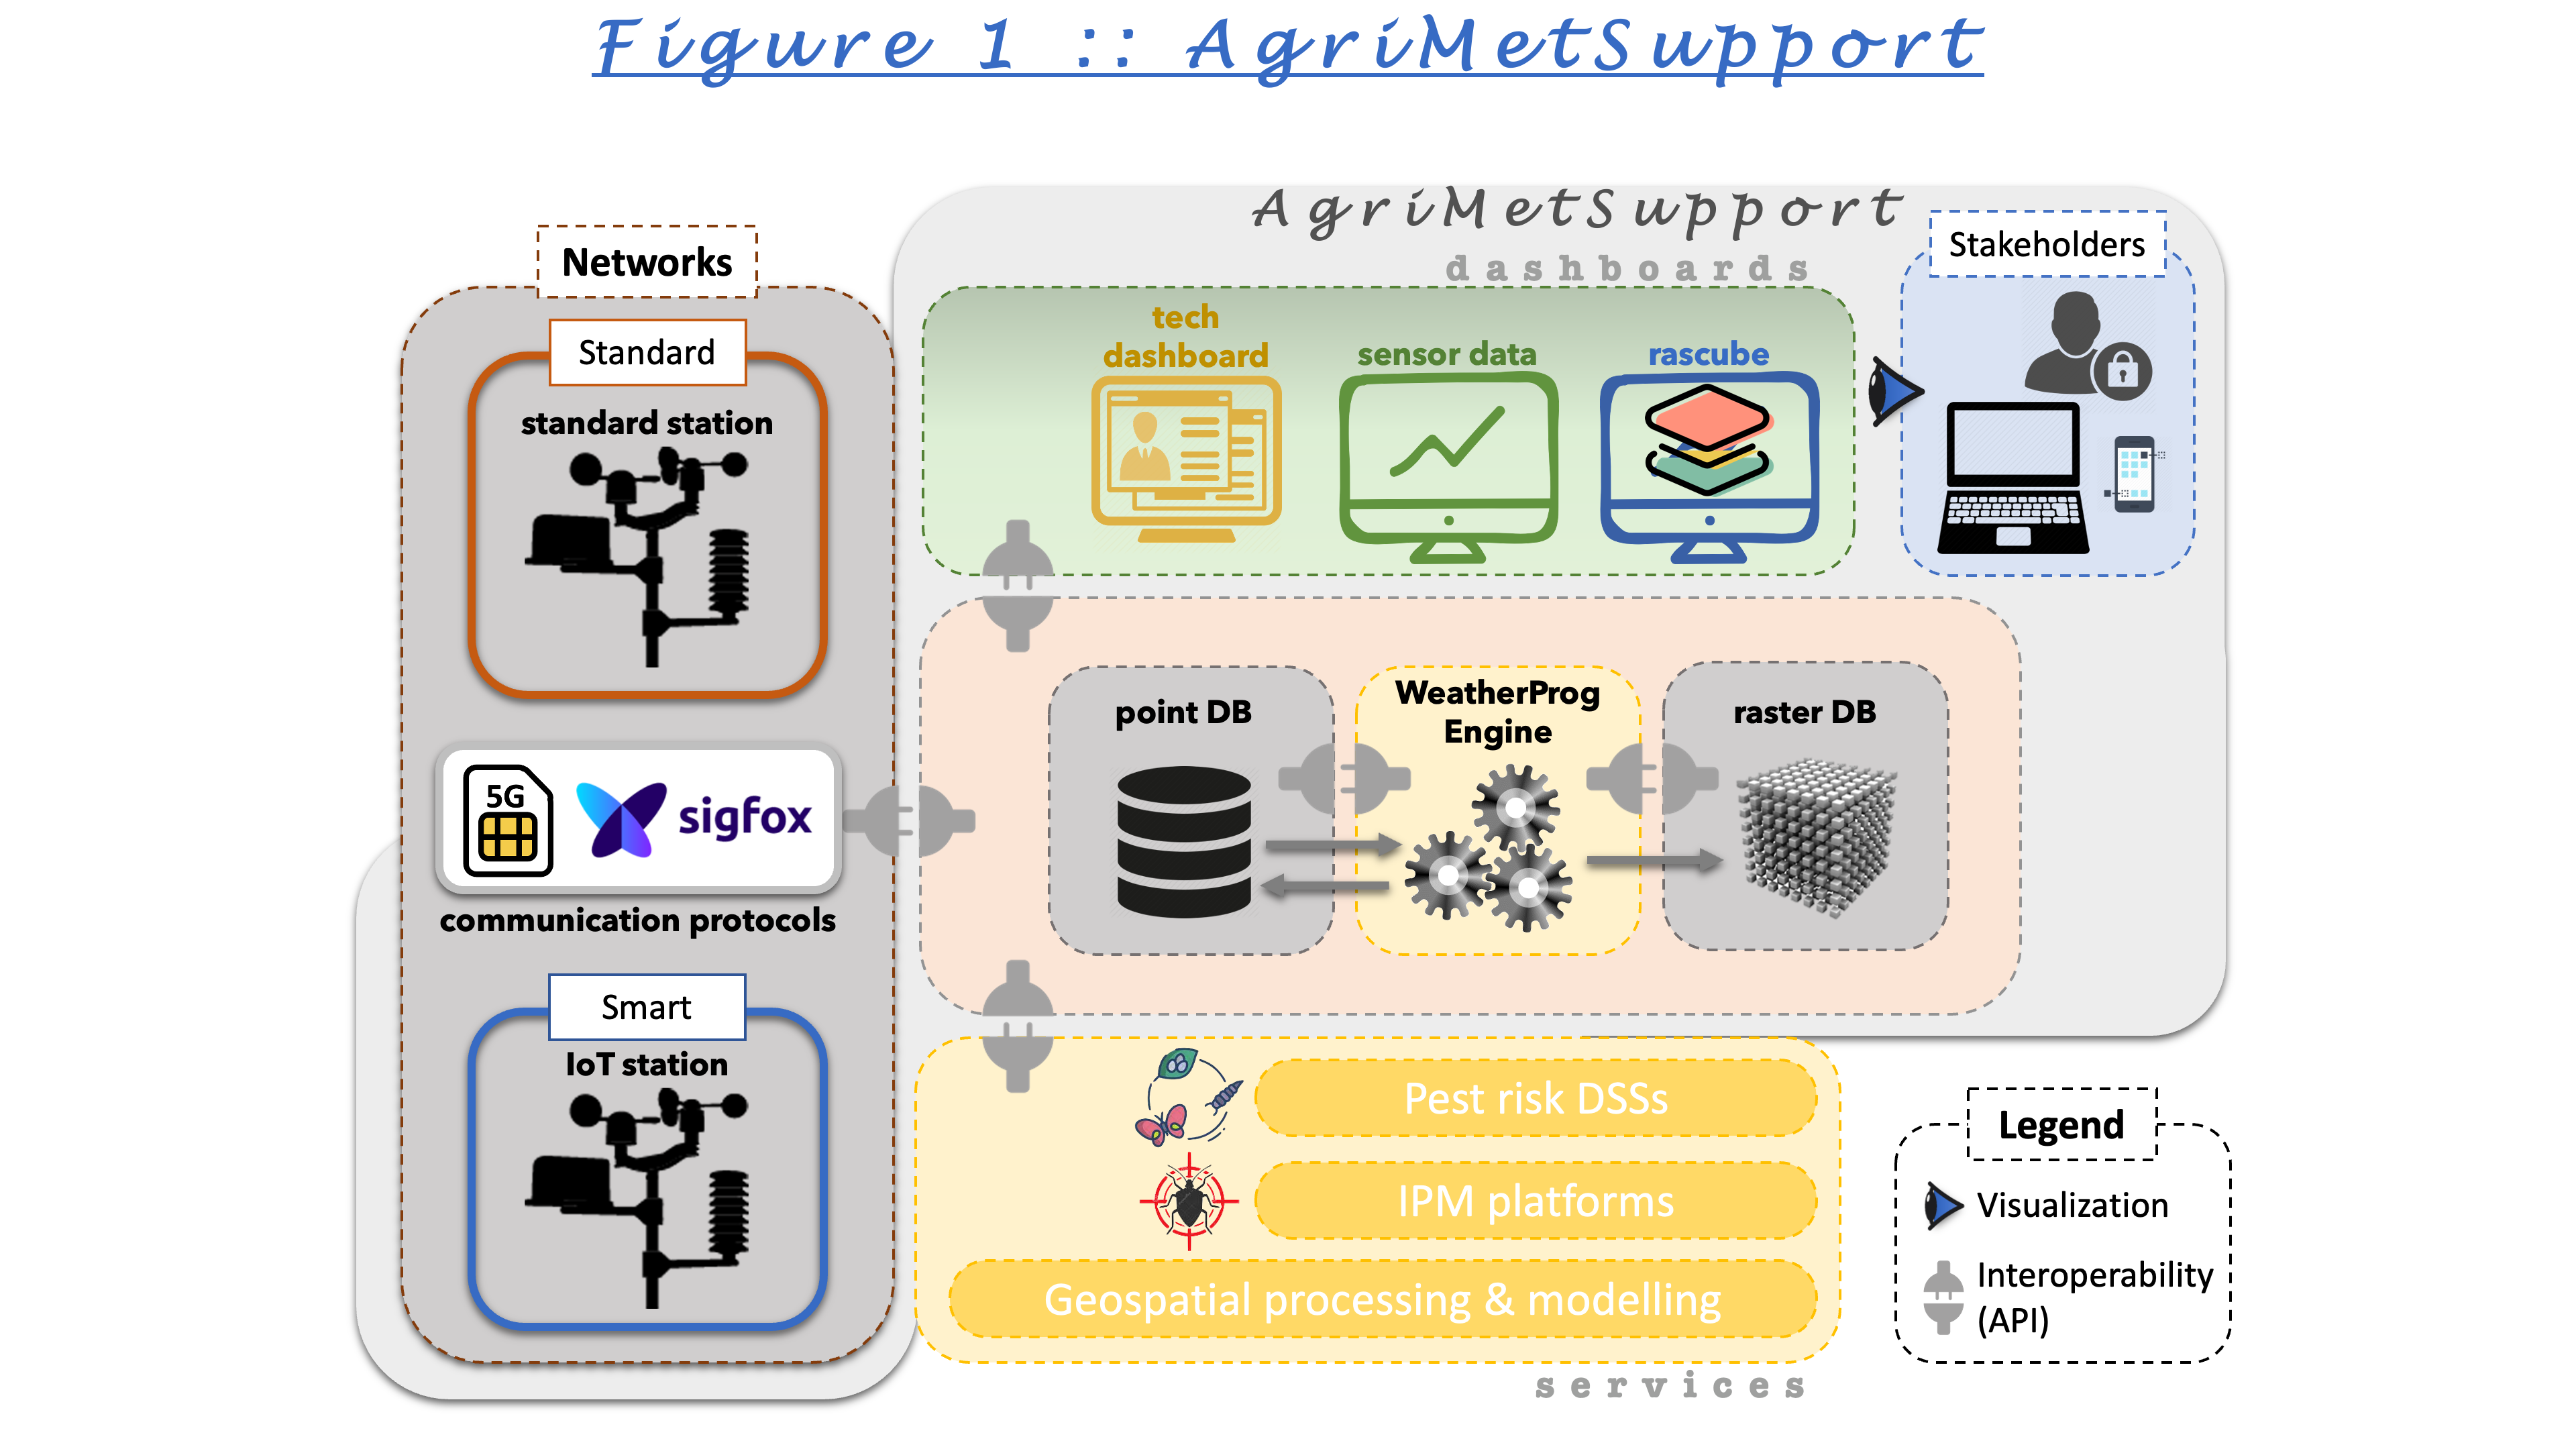
\includegraphics[angle=0,scale=.56,trim=4.6cm 0cm 2cm 2.4cm,clip]{figures/Fig01_AgriMetSupport.png}
	\DIFaddendFL \caption{
            \DIFdelbeginFL \DIFdelFL{High level }\DIFdelendFL \DIFaddbeginFL \DIFaddFL{High-level }\DIFaddendFL architecture of the \DIFdelbeginFL \DIFdelFL{AgriMetSupport }\DIFdelendFL \DIFaddbeginFL \DIFaddFL{Agri\-Met\-Support }\DIFaddendFL cyber-physical system. The \DIFdelbeginFL \DIFdelFL{non-pysical parts of }\DIFdelendFL \DIFaddbeginFL \DIFaddFL{figure illustrates }\DIFaddendFL the \DIFdelbeginFL \DIFdelFL{whole }\DIFdelendFL \DIFaddbeginFL \DIFaddFL{integration of sensors, communication networks, WMO-compliant point database, data processing modules by WeatherProg, OGC-compliant raster database, and user interaction dashboards in an interoperable }\DIFaddendFL system\DIFdelbeginFL \DIFdelFL{- including the Services block - }\DIFdelendFL \DIFaddbeginFL \DIFaddFL{. Interoperability }\DIFaddendFL is \DIFdelbeginFL \DIFdelFL{running }\DIFdelendFL \DIFaddbeginFL \DIFaddFL{addressed through internal and external APIs. The system is hosted }\DIFaddendFL at the Granatellum data center\DIFaddbeginFL \DIFaddFL{, }\DIFaddendFL managed by CRISP and located at the Department of Agriculture, University of Napoli Federico II.
 }
	\label{cyberPhysicalSystemFig}
\end{figure}
\DIFdelbegin %DIFDELCMD < 

%DIFDELCMD < %%%
\DIFdel{Peripheral components are the actual monitoring networks.
In fact, }\DIFdelend %DIF > Peripheral physical components are the actual monitoring networks.
Agri\-Met\-Support is capable of handling and integrating data coming from multiple heterogeneous networks of stations, possibly under the responsibility of different stakeholders working in the same territory.
Each network can include different kinds of station \DIFaddbegin \DIFadd{and sensor}\DIFaddend , and each network can submit data to AgriMetSupport in different formats, since the decoding module of WeatherProg can be configured to accommodate such differences.
The opportunity to integrate networks is of paramount importance to \DIFdelbegin \DIFdel{systematically }\DIFdelend \DIFaddbegin \DIFadd{sys\-tem\-at\-ic\-al\-ly
 }\DIFaddend optimise the joint management of public and/or private monitoring infrastructures with significant beneficial impact on cost saving and services enhancement.

%and reciprocal impact both on the different agencies sharing their data and on farmers and end users who can enjoy more accurate data and less uncertain services.

AgriMetSupport can be employed also in contexts where there is an insufficient monitoring network coverage of the territory.
In fact, it comes with its own monitoring network, characterised by smart stations which are particularly suitable for temporary deployments and for fine tuning the parameters of the various models included in the \DIFdelbegin \DIFdel{GCI }\DIFdelend \DIFaddbegin \DIFadd{CPS }\DIFaddend \citep{Martino2019AFI}.
It must be stressed that the smart monitoring network is entirely optional, being a component like the others that can be simply removed if there is either an already excellent coverage of the territory or any micro-climatic monitoring is needed, therefore not preventing the use of AgriMetSupport in such scenarios. %\note{[add installation of low cost station by farmers]}

\DIFdelbegin \DIFdel{The AgriMetSupport }\DIFdelend \DIFaddbegin \statusblock{}{wip}{%Interoperability.\\
%In addition, more tailored services are provided through dedicated interfaces to automatically retrieve data. %(e.g. by means of a REST API).
Here, I present an overview of CPS interoperability within Agri\-Met\-Support.
As an interoperable CPS, it integrates multiple internal and external APIs, as illustrated in \cref{cyberPhysicalSystemFig}.
One external API is dedicated to handling HTTPS requests from stations transmitting coded messages containing sensor measurements. A PHP-based server listens for these requests, after which WeatherProg decodes the incoming data and ingests it into the database.
Another web API allows machine-to-machine requests, supporting Findability, Accessibility, Interoperability, and Reuse (FAIR) principles for digital assets. This API not only serves as a data delivery service for stakeholders but also enables the deployment of custom web applications, including tailored web mapping dashboards. These applications can even operate independently outside the Agri\-Met\-Support infrastructure, feeding external services.
Additionally, two internal APIs manage CRUD (Create, Read, Update, Delete) operations over the point and raster databases, ensuring seamless integration and data accessibility within the system.
Together, these APIs ensure efficient data collection, processing, and dissemination, enhancing the system’s interoperability and usability.
}

\DIFadd{The Agri\-Met\-Support }\DIFaddend infrastructure is based on the distinction amongst data, logic and visualisation tiers \DIFaddbegin \DIFadd{(\mbox{%DIFAUXCMD
\cref{Fig_tiers}}\hskip0pt%DIFAUXCMD
)}\DIFaddend .
The data tier is made by different data\-bases.
One database \DIFaddbegin \DIFadd{(external data sources in \mbox{%DIFAUXCMD
\cref{Fig_tiers}}\hskip0pt%DIFAUXCMD
) }\DIFaddend is usually maintained by a local government agency \DIFdelbegin \DIFdel{(}\DIFdelend or any other entrusted/responsible entity \DIFaddbegin \DIFadd{(}\DIFaddend such as the Campania Region departments shown in Section \ref{sec:casestudy}) which is in charge of retrieving raw records by the monitoring stations within its network.
\DIFdelbegin \DIFdel{A second database }\DIFdelend \DIFaddbegin 

\begin{figure}[!t] %DIF >  [H] ensures the figure appears exactly here
	\centering %DIF >  trim=left bottom right top
	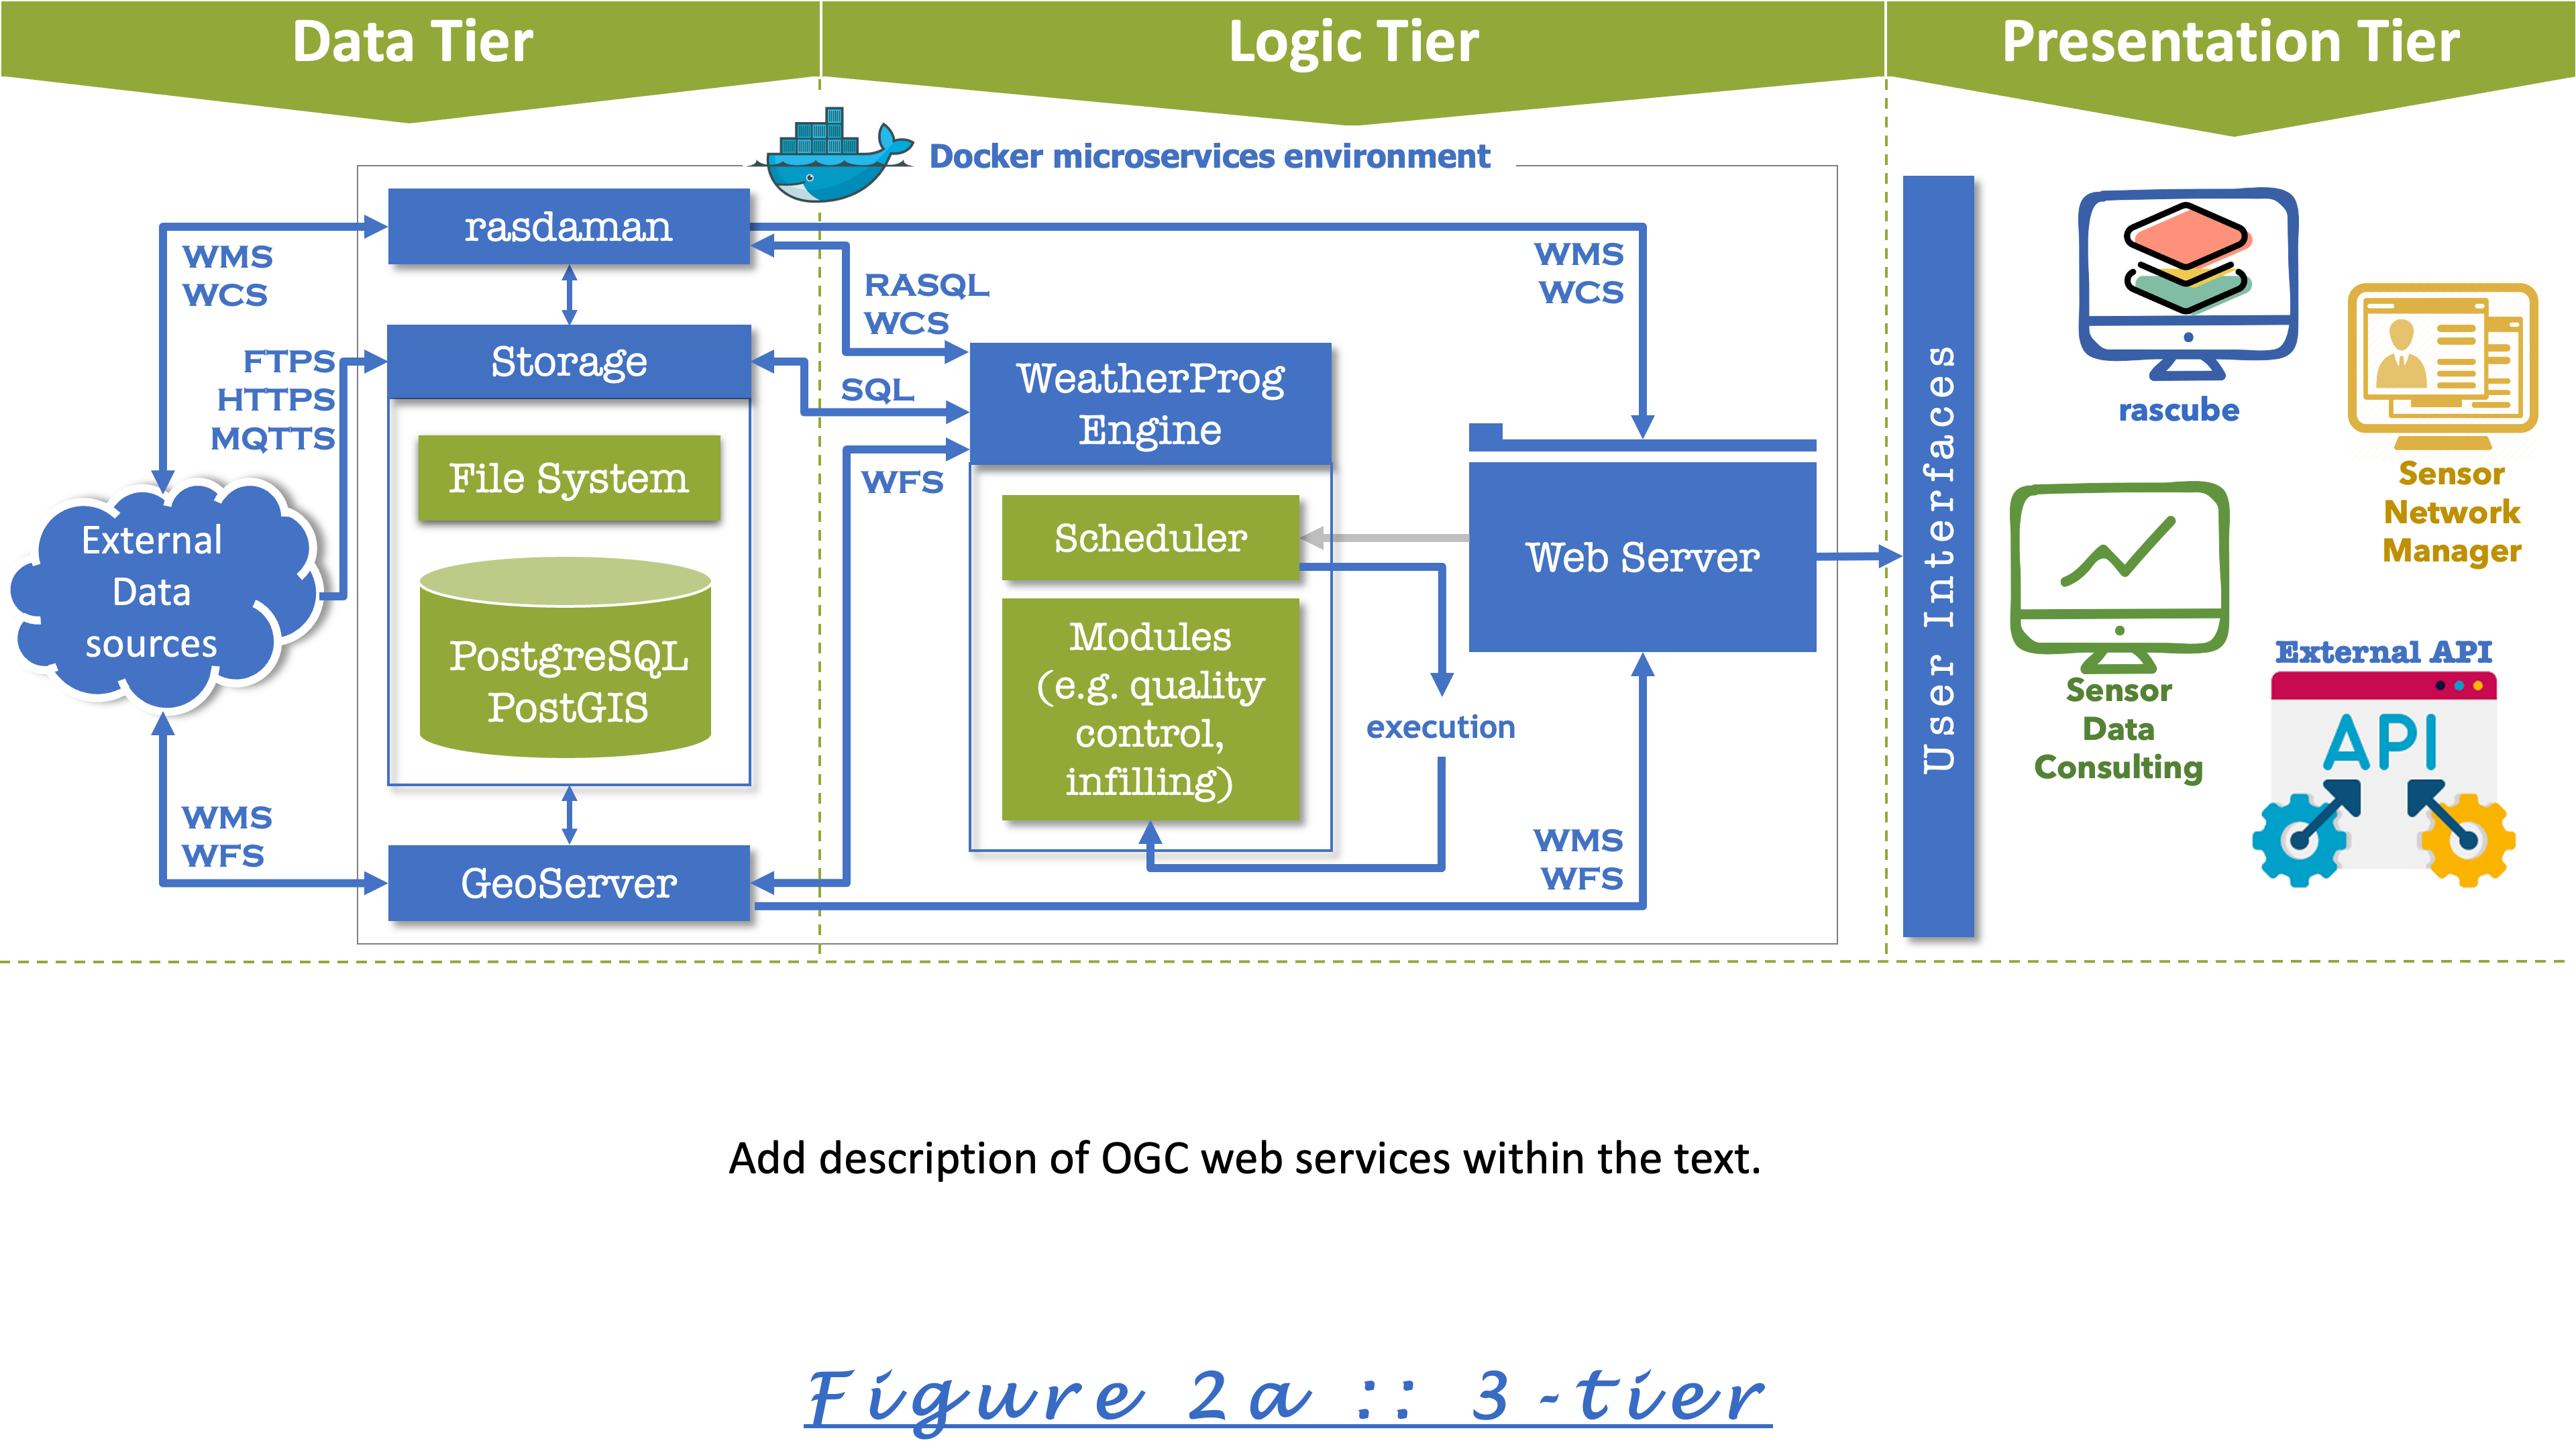
\includegraphics[angle=0,scale=.4,trim=0cm 6.2cm 0cm 0cm,clip]{figures/Fig02_Tiers.png}
	\caption{ \DIFaddFL{(get the latest figure version from powerpoint) The three-tier infrastructure of the AgriMetSupport system. The data tier includes external and internal data sources (and APIs) such as sensors, file systems, geospatial datasets (vector and raster), and distinct databases (PostgreSQL and rasdaman). The logic tier processes the data using the WeatherProg Engine (all modules are shown in Figure 3), enabling for instance quality control and infilling used in the validation study. The presentation tier provides user-facing interfaces such as dashboards and APIs, including internal APIs for Agri\-Met\-Support and web APIs for external services (see \mbox{%DIFAUXCMD
\cref{cyberPhysicalSystemFig}}\hskip0pt%DIFAUXCMD
). The Docker microservices environment orchestrates the backend components within the data and logic tiers, ensuring seamless communication and scalability.}}
	\label{Fig_tiers}
\end{figure}

\DIFadd{A second postgreSQL database with postGIS extension }\DIFaddend is the main \DIFdelbegin \DIFdel{AgriMetSupport }\DIFdelend \DIFaddbegin \DIFadd{Agri\-Met\-Support }\DIFaddend WMO-compliant relational database  \DIFdelbegin \DIFdel{(see the point database in \mbox{%DIFAUXCMD
\cref{cyberPhysicalSystemFig}}\hskip0pt%DIFAUXCMD
) in }\DIFdelend \DIFaddbegin \DIFadd{in }\DIFaddend which decoded raw measurements possibly coming from different networks are stored (e.g. from local entrusted entities and from private stakeholders using smart stations).
This database supports \DIFdelbegin \DIFdel{all the }\DIFdelend WeatherProg modules execution and produces qualified data for agriculture meteorology management and planning.
%The first is a WMO-compliant relational data base used to store station measurements.
%The main central components are the WeatherProg core engine and the data bases. 
%Two main data bases are employed by AgriMetSupport.
A third \DIFdelbegin \DIFdel{database is optional (not shown in \mbox{%DIFAUXCMD
\cref{cyberPhysicalSystemFig}}\hskip0pt%DIFAUXCMD
) }\DIFdelend \DIFaddbegin \DIFadd{postgreSQL database with postGIS extension is optional }\DIFaddend and supports the management of smart stations data which are then ingested in the main point database.
The latter is \DIFdelbegin \DIFdel{a raster data base capable of handling the }\DIFdelend \DIFaddbegin \DIFadd{an OGC-compliant raster database (rasdaman in \mbox{%DIFAUXCMD
\cref{Fig_tiers}}\hskip0pt%DIFAUXCMD
) designed to manage }\DIFaddend digital climatic maps\DIFdelbegin \DIFdel{which can be produced }\DIFdelend \DIFaddbegin \DIFadd{, which the WeatherProg engine can generate }\DIFaddend as spatio-temporal tiles\DIFdelbegin \DIFdel{by the WeatherProg engine.
An }\DIFdelend \DIFaddbegin \DIFadd{.
This }\DIFaddend array database is used to stitch together the 2D maps or tiles calculated over time for the different agroclimatic variables to produce multi-dimensional arrays or data cubes, which can be  characterised by three (X, Y, Time) or four (X, Y, Time, Variable) dimensions.
Subsetting operations on these data cubes including trimming and slicing are embarrassingly parallel and scale up according to the number of available CPU cores.
This enables the production of performing dashboards in the presentation tier\DIFaddbegin \DIFadd{, }\DIFaddend enabling the visualization of climatic maps.
%The rasdaman DBMS \citep{baumann:rasdaman} has been chosen due to its representation of spatial data as datacubes, i.e. digital maps with more than two dimensions, where the third dimension is used to represent time.

The logic tier is \DIFdelbegin \DIFdel{centralised in AgriMetSupport and is made mostly by }\DIFdelend \DIFaddbegin \DIFadd{centralized in Agri\-Met\-Support and is primarily composed of }\DIFaddend the WeatherProg engine (Section \ref{sec:weatherprog}) and \DIFdelbegin \DIFdel{by web servers }\DIFdelend \DIFaddbegin \DIFadd{web services }\DIFaddend capable of connecting \DIFdelbegin \DIFdel{AgriMetSupport to the }\DIFdelend \DIFaddbegin \DIFadd{Agri\-Met\-Support to }\DIFaddend external databases and \DIFdelbegin \DIFdel{to the }\DIFdelend smart stations.

\DIFaddbegin \begin{figure}[!t] %DIF >  [H] ensures the figure appears exactly here
	\centering %DIF >  trim=left bottom right top
	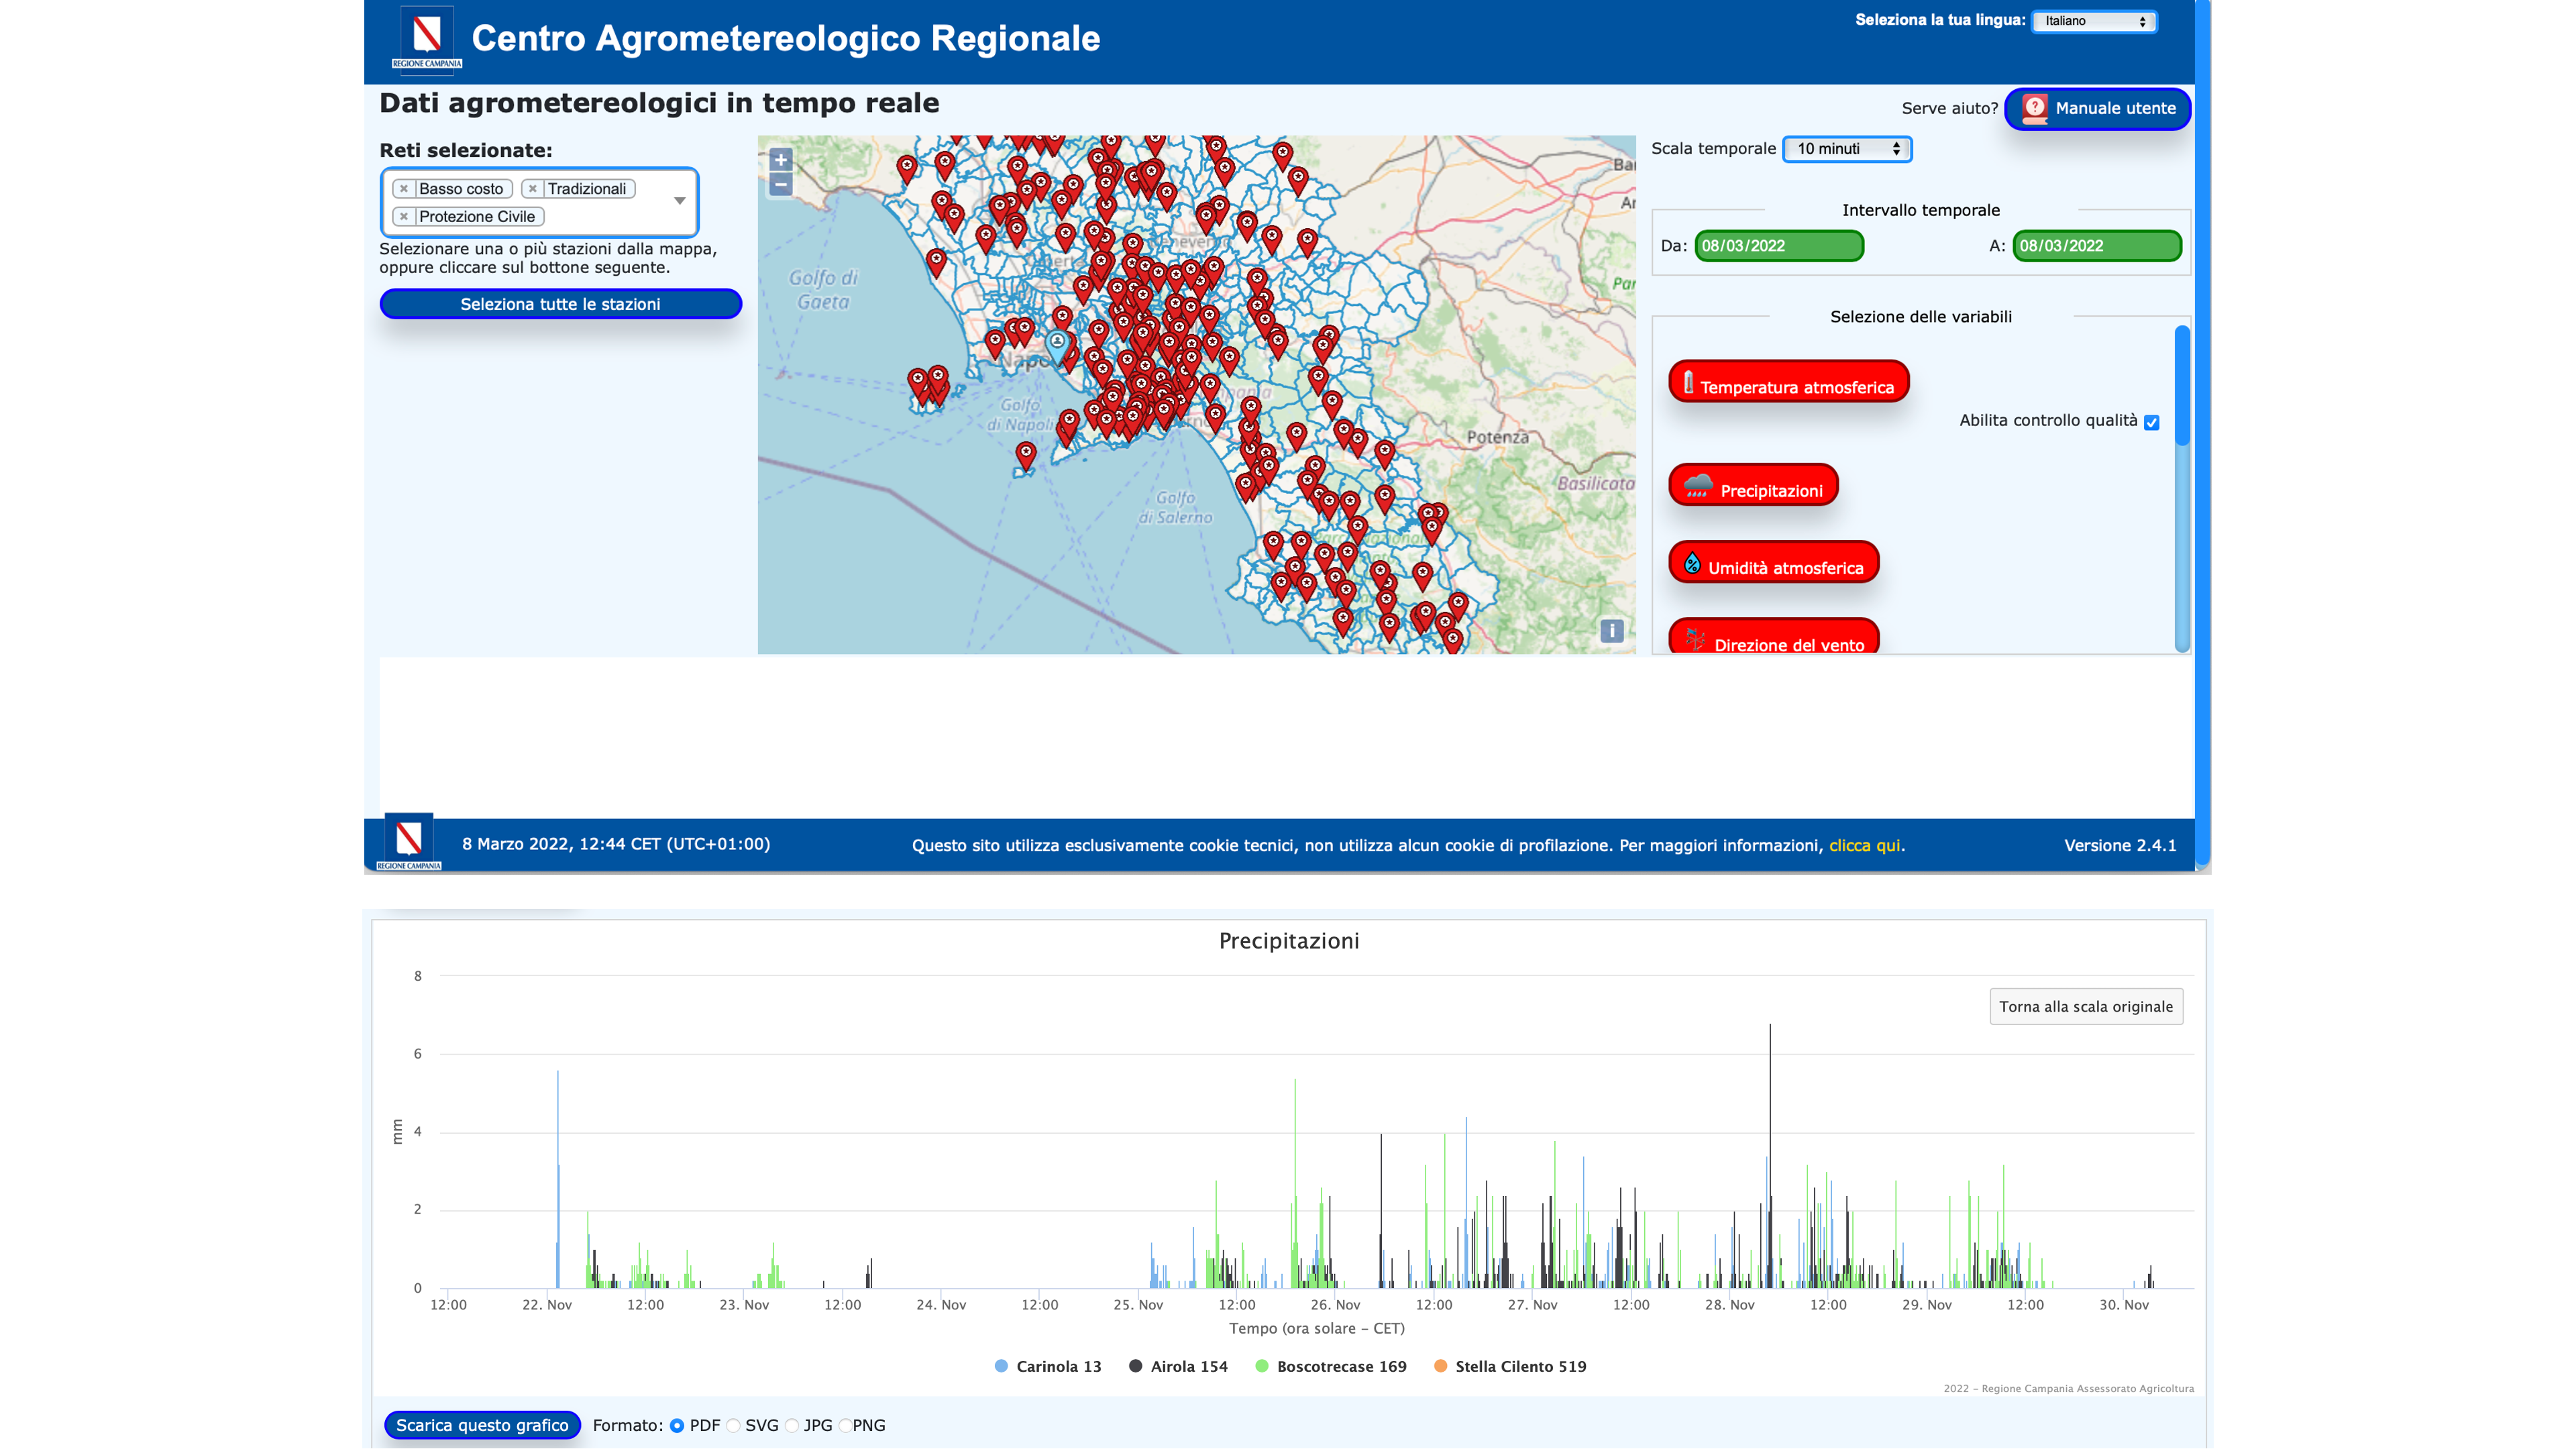
\includegraphics[angle=0,scale=.4,trim=0cm 0cm 0cm 0cm,clip]{figures/Fig03_SensorDataConsultingApp.png}
	\caption{ \DIFaddFL{Web application for consulting sensor data. 
              An example of rainfall time series for four selected stations is displayed at the bottom.}}
	\label{Fig_webapp}
\end{figure}

\DIFaddend Finally, the presentation tier includes various end-user interfaces providing a number of different services.
A data consulting web application publishes the agroclimatic data managed by the cyber-physical system to the general public \DIFaddbegin \DIFadd{(\mbox{%DIFAUXCMD
\cref{Fig_webapp}}\hskip0pt%DIFAUXCMD
)}\DIFaddend .
It is in charge of providing a public or restricted access to the basic agrometeorological data (distinguishing between raw and quality controlled data) and to agrometeorological derived information, such as the consultation of bio-climatic indices rather than a pest risk service\DIFdelbegin \DIFdel{(the pest risk module within WeatherProg is under development).
In addition, more tailored services are provided through dedicated interfaces to automatically retrieve data. %DIF < (e.g. by means of a REST API).
There exists an Application Programming Interface (API) via web allowing machine-to-machine requests and enabling data retrieval in the context of Findability, Accessibility, Interoperability, and Reuse (FAIR) of digital assets.
Beyond a delivery service available for any stakeholder, the web-API can be used to deploy dedicated web applications including tailored web mapping dashboards, even allowing for independent operation outside of the AgriMetSupport infrastructure. 
}\DIFdelend \DIFaddbegin \DIFadd{.
}\DIFaddend %A web-based interface is also available for officers in charge of the system to tune the operational parameters of WeatherProg's models. \note{really?}

\section{WeatherProg engine}\label{sec:weatherprog}
\subsection{Main modules}
WeatherProg \citep{langella:weatherprog2014} is a computer program to automatically manage agrometeorological data.
The first implementation was carried out as the baseline asynchronous engine for the raw weather records handling in the (LIFE08 ENV/IT/000408) SOILCONS-WEB project.
It was developed because the main input requirements of the different modelling chains embedded in the project DSS \citep{Terribile:soilconsweb:2015} were the availability of both (i) complete and homogeneous time series and (ii) spatially exhaustive digital maps of the key agrometeorological variables (e.g. temperature and precipitation).

After the end of the project, the program has been progressively modified and updated in order to accommodate the requirements of both local government agencies (such as Italian Regions) and farmers, also thanks to an innovative cyber-physical infrastructure which WeatherProg is embedded in\DIFdelbegin \DIFdel{(\mbox{%DIFAUXCMD
\cref{cyberPhysicalSystemFig}}\hskip0pt%DIFAUXCMD
)}\DIFdelend .
Indeed, WeatherProg can facilitate the work by a local administrative body which is in charge of managing and publishing agrometeorological data and of promoting measures for low pesticide-input pest management \citep{eu:dir128:2009}, for instance by producing bulletins based on bioclimatic indicators or on the results of pest simulation models.
WeatherProg can facilitate the work by a farmer too, since it supports for instance the implementation of an integrated pest management tool \citep{Terribile:dssvitis:2017} by configuring services in the context of Agriculture 4.0 and advanced IoT \DIFdelbegin \DIFdel{framework as depicted in \mbox{%DIFAUXCMD
\cref{cyberPhysicalSystemFig}}\hskip0pt%DIFAUXCMD
}\DIFdelend \DIFaddbegin \DIFadd{frameworks}\DIFaddend .

\DIFaddbegin \begin{figure}[!t] %DIF >  [H] ensures the figure appears exactly here
	\centering %DIF >  trim=left bottom right top
	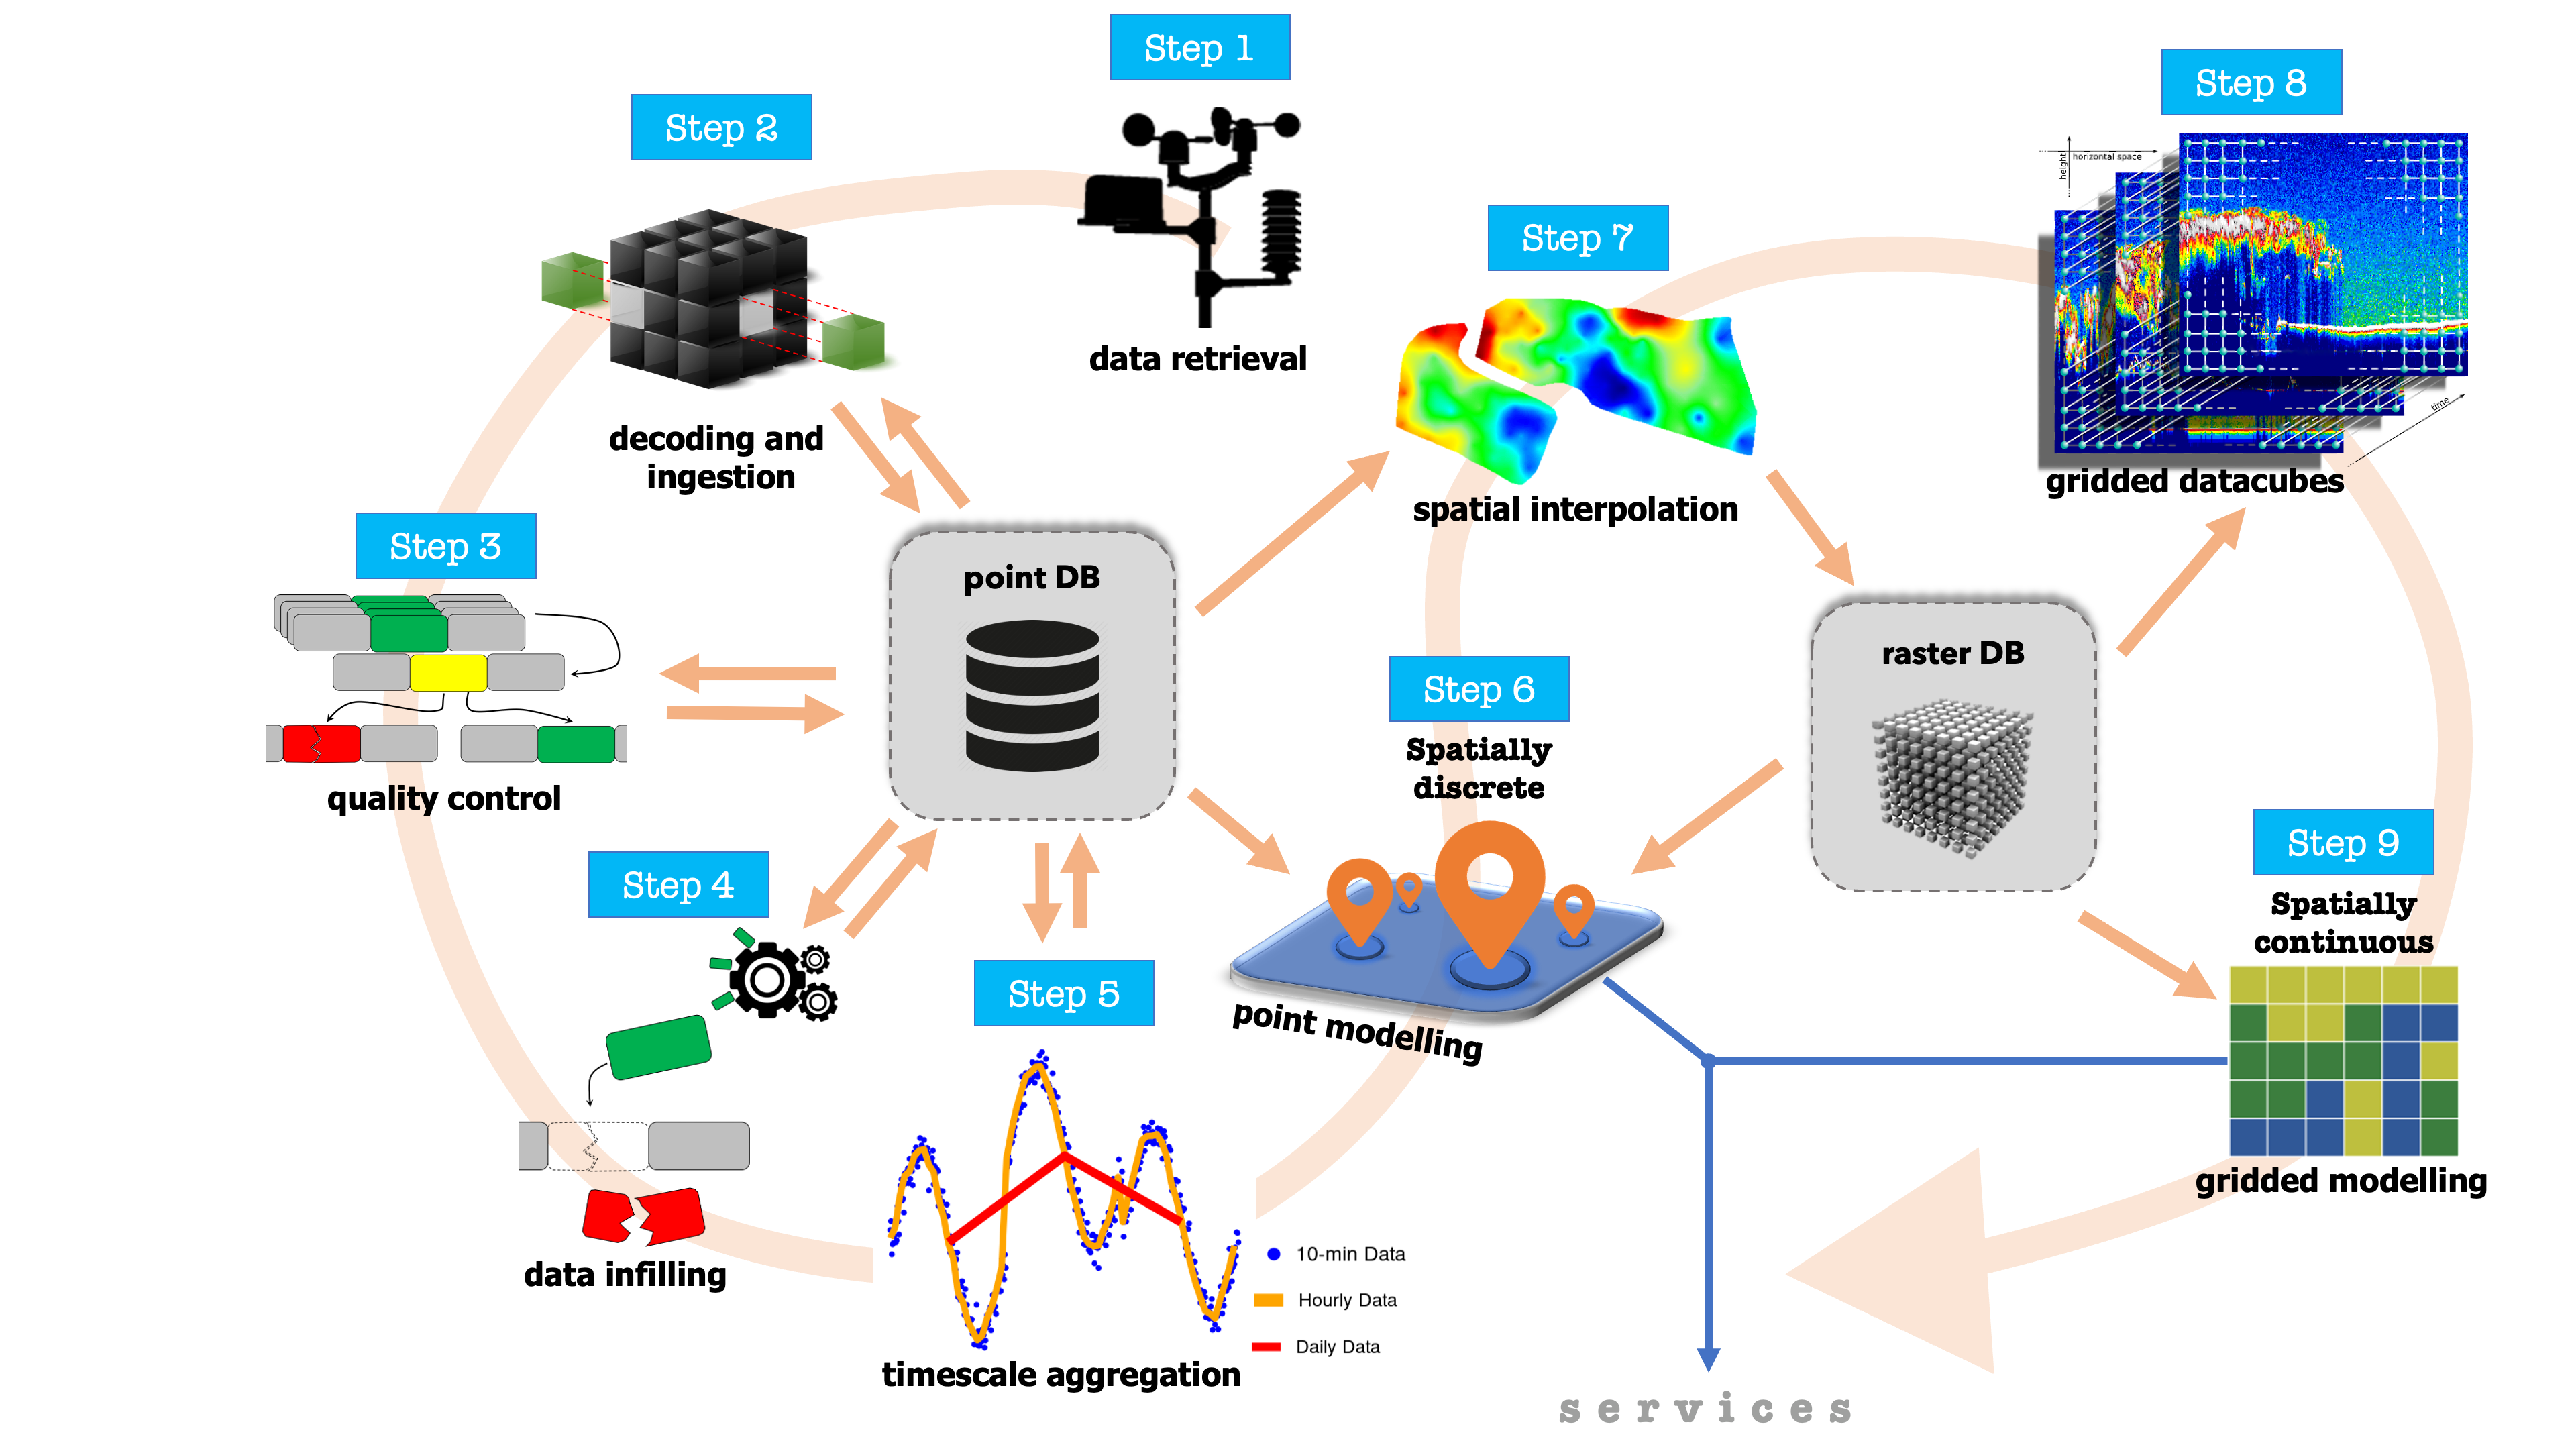
\includegraphics[angle=0,scale=.45,trim=3cm 0cm 0cm 0cm,clip]{figures/Fig03_WeatherProg_modules.png}
	\caption{
            \DIFaddFL{Modules of the WeatherProg Engine and their functionalities. Raw data from sensors undergo a series of processing steps, including decoding, quality control, infilling, temporal aggregation, and spatial interpolation. The resulting processed data, available as point-based and raster-based formats, is utilized both internally (via internal APIs for feeding dashboards within Agri\-Met\-Support) and externally (via web APIs) to support decision-making systems and broader applications, as illustrated in \mbox{%DIFAUXCMD
\cref{cyberPhysicalSystemFig}}\hskip0pt%DIFAUXCMD
.
 }}
	\label{Fig:WeatherProg}
\end{figure}

\DIFaddend Nowadays, WeatherProg \DIFaddbegin \DIFadd{(\mbox{%DIFAUXCMD
\cref{Fig:WeatherProg}}\hskip0pt%DIFAUXCMD
) }\DIFaddend is a geospatial engine that can be embedded in a web-based DSS dedicated to real-time and on-the-fly consulting of both agrometeorological and derived variables in the form of spatial-point time series or in the form of geospatial maps.
Raw reports from a climatological network can be ingested and a different set of operations are performed ranging from the data checking to the delivery of gridded agrometerological variables.
Temperature, rainfall, relative humidity, solar radiation, atmospheric pressure and wind speed are the most commonly handled variables by the program at different time scales.

\DIFdelbegin \DIFdel{WeatherProg starts automatically at predefined time intervals when a new report from the monitoring network is available (which depends upon the station data logger query frequency and not on the measurement frequency), and }\DIFdelend \DIFaddbegin \DIFadd{A scheduler within the WeatherProg engine handles the automatic execution of modules and }\DIFaddend carries out the following main operations \DIFaddbegin \DIFadd{(\mbox{%DIFAUXCMD
\cref{Fig:WeatherProg} }\hskip0pt%DIFAUXCMD
and \mbox{%DIFAUXCMD
\cref{Box01:WeatherProg_Operations}}\hskip0pt%DIFAUXCMD
)}\DIFaddend :
\begin{enumerate}
    \item \DIFdelbegin \DIFdel{Complete data retrieval. The }\DIFdelend \DIFaddbegin \DIFadd{Data retrieval. There are two main streams to get new measurements in the data tier of Agri\-Met\-Support, either from data providers or directly from the stations. 
    In the first case, }\DIFaddend real-time \DIFdelbegin \DIFdel{report }\DIFdelend \DIFaddbegin \DIFadd{reports -- e.g. a Comma Separated Value (CSV) file -- }\DIFaddend with measurements from all sensors and stations belonging to a monitoring network \DIFdelbegin \DIFdel{arrives to WeatherProg via either SFTPor HTTPSsecure protocol}\DIFdelend \DIFaddbegin \DIFadd{is delivered hourly via the Secure File Transfer Protocol (SFTP).
    The second data stream enables any station to directly send every 10 minutes its instantaneous measurements as hexadecimal string via the Hypertext Transfer Protocol Secure (HTTPS)}\DIFaddend .

    \item Data decoding and ingestion. \DIFdelbegin \DIFdel{After the report is decoded according to time scale and sensors, data are ingested in the the main AgriMetSupport }\DIFdelend \DIFaddbegin \DIFadd{Each data provider uses custom labels for the variables and custom date formats, therefore WeatherProg knows how to read the CSV file, to decode its content and to ingest it in the main Agri\-Met\-Support }\DIFaddend WMO-compliant relational database. 
    \DIFaddbegin \DIFadd{The hexadecimal string is decoded into meaningful data (see the concrete example in \mbox{%DIFAUXCMD
\cref{Box01:WeatherProg_Operations}}\hskip0pt%DIFAUXCMD
) and seamlessly integrated into the database.
    In both cases, the ingestion of these raw records is made by means of SQL queries via an internal API (which is shown in \mbox{%DIFAUXCMD
\cref{cyberPhysicalSystemFig} }\hskip0pt%DIFAUXCMD
between the WeatherProg engine and the point DB boxes).
}\DIFaddend 

    \item Quality control and flagging of data. Quality control \DIFdelbegin \DIFdel{of time series are }\DIFdelend \DIFaddbegin \DIFadd{is }\DIFaddend performed to automatically demarcate good measurements from wrong and missing values, which are conveniently flagged for the subsequent \DIFdelbegin \DIFdel{and optional infilling procedure}\DIFdelend \DIFaddbegin \DIFadd{procedures}\DIFaddend .
    An anomalous datum is detected thanks to a multilevel technology based on interlinked quality control types such as range, continuity, climatological, spatial, temporal and persistency.
    Certification of abnormality can be semi-automatic other than automatic.
    The semi-automatic procedure is the result of the combination of both the data-driven WeatherProg checking procedure and the knowledge-based human checking in order to finally assign the definitive flag\DIFdelbegin \DIFdel{(for details see Section \ref{sec:qcheck})}\DIFdelend .

    \DIFaddbegin \begin{figure}[!t] %DIF >  [H] ensures the figure appears exactly here
    	\centering %DIF >  trim=left bottom right top
    	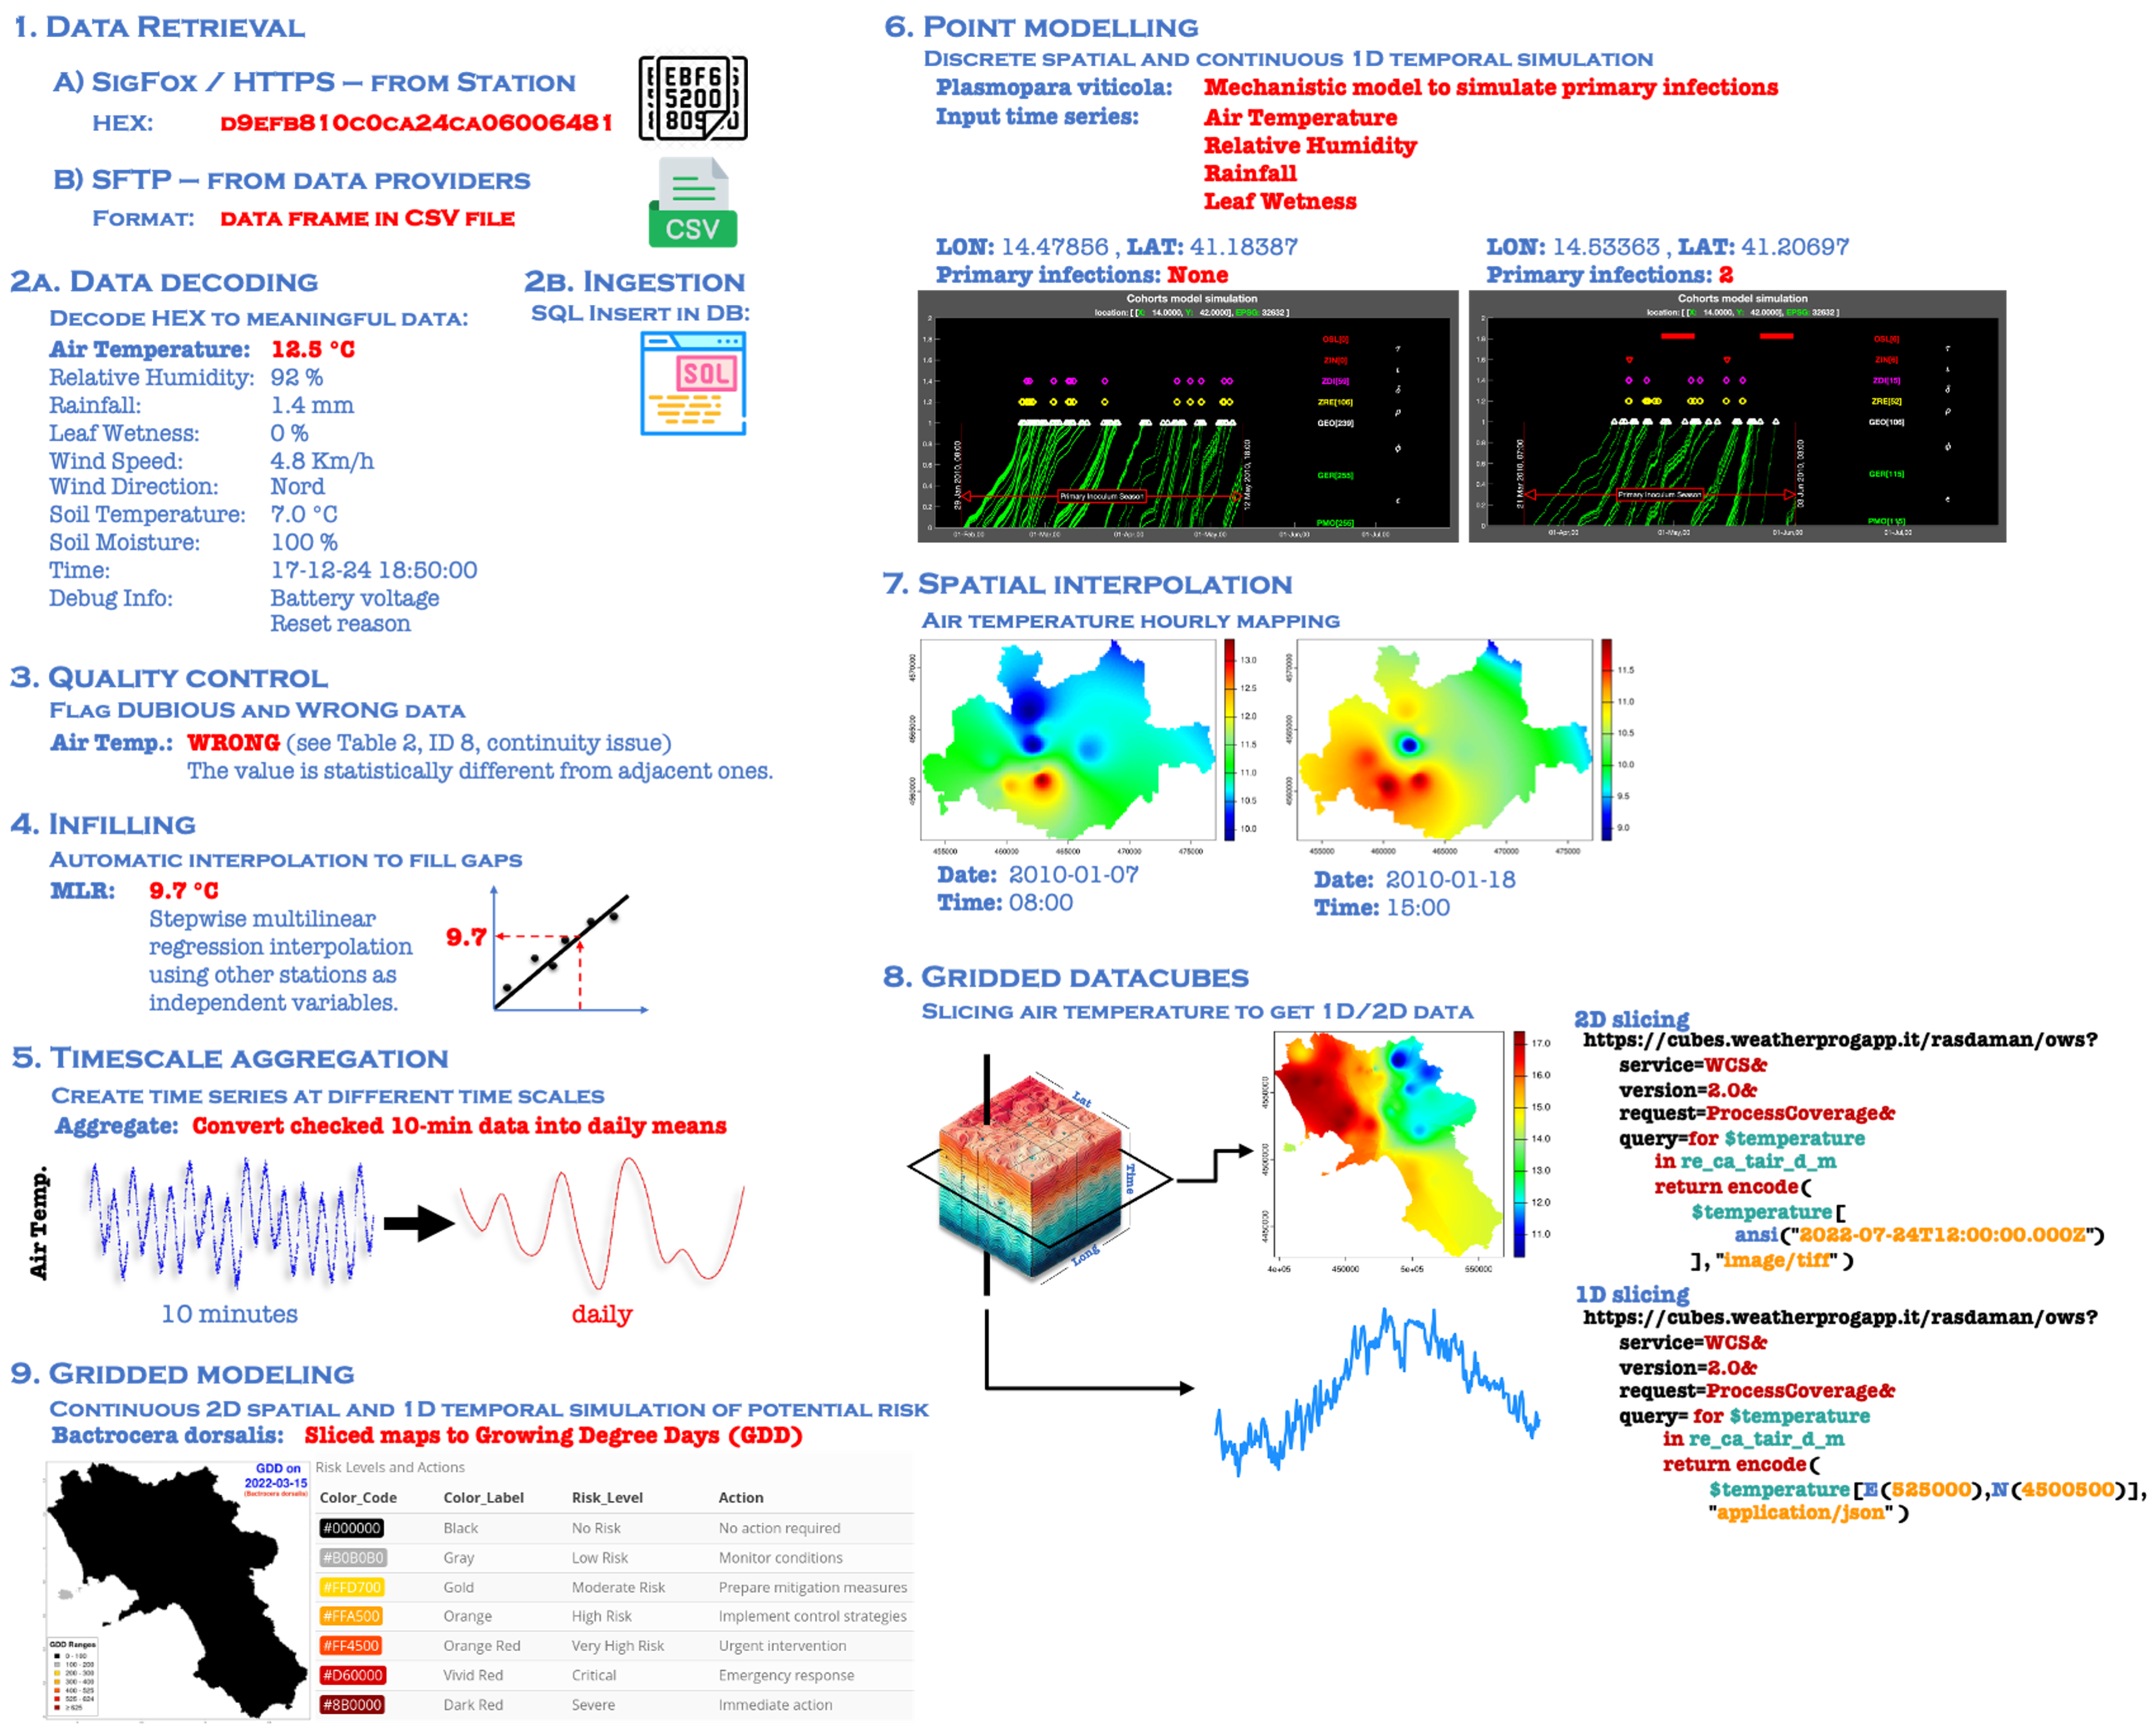
\includegraphics[angle=0,scale=.45,trim=0cm 0cm 0cm 0cm,clip]{figures/Box01_WeatherProg_concreteOperations.png}
    	\caption{\DIFaddFL{NOTES: Change the black map in point (9); CAPTION: Concrete examples about WeatherProg modules.}}
    	\label{Box01:WeatherProg_Operations}
    \end{figure}

    \DIFaddend \item Data infilling. Anomalies and missing \DIFdelbegin \DIFdel{data are all flaggedto be %DIF < interpolated by means of an automatic linear regression procedure.
    infilled in order to get }\DIFdelend \DIFaddbegin \DIFadd{values are systematically flagged, allowing the optional infilling procedure to create }\DIFaddend complete and homogeneous time series. %DIF >  enabling the creation of structured time series
    Different methods are available such as a deterministic approach based on moving average with a growing temporal kernel, or a statistical method using a stepwise multilinear regression.
    \DIFdelbegin \DIFdel{It }\DIFdelend \DIFaddbegin \DIFadd{The latter }\DIFaddend uses data from other stations and \DIFdelbegin \DIFdel{it }\DIFdelend performs an iterative optimization procedure to properly select the time series length and the regression covariates for infilling each single anomaly or gap.
    \DIFdelbegin \DIFdel{For more details see \mbox{%DIFAUXCMD
\cref{sec:infill}}\hskip0pt%DIFAUXCMD
. }\DIFdelend \DIFaddbegin \DIFadd{In the example of \mbox{%DIFAUXCMD
\cref{Box01:WeatherProg_Operations}}\hskip0pt%DIFAUXCMD
, the raw air temperature value of \mbox{%DIFAUXCMD
\SI{12.5}{\degreeCelsius} }\hskip0pt%DIFAUXCMD
was flagged as wrong due to the continuity check, and an interpolated value of \mbox{%DIFAUXCMD
\SI{9.7}{\degreeCelsius} }\hskip0pt%DIFAUXCMD
was obtained. Using nine stations with approximately 300 measurements centered around the erroneous value, the cross-validation RMSE in the neighborhood was \mbox{%DIFAUXCMD
\SI{0.28}{\degreeCelsius}}\hskip0pt%DIFAUXCMD
, underscoring the high goodness of fit. 
    %DIF > For more details see \cref{sec:infill}.
}\DIFaddend 

    \item Time scale aggregation. Variables are aggregated over time using \DIFdelbegin \DIFdel{different statistics (}\DIFdelend \DIFaddbegin \DIFadd{standard statistical measures -- such as }\DIFaddend minimum, maximum, average, sum, \DIFdelbegin \DIFdel{most frequent, and so forth) computed on 10-minutes measurementsafter the quality control }\DIFdelend and \DIFdelbegin \DIFdel{possibly the infill procedures are fulfilled.
    }\DIFdelend \DIFaddbegin \DIFadd{mode -- computed from 10-minute measurements. 
    These calculations take place only after quality control has been applied.
    Infilled data are excluded, and only quality-controlled measurements of high reliability are included in the calculations; if they are insufficient, a missing value is created instead.
    This step generates new data forming time series at various temporal scales, such as hourly and daily.
    These newly generated data are considered raw and will undergo quality control and optional infilling.
    %DIF > Variables are aggregated over time using standard statistics (minimum, maximum, average, sum, most frequent, and so forth) computed on 10-minutes measurements after the quality control and possibly the infill procedures are fulfilled.
    }\DIFaddend %computed on the most fundamental units of measurements, that is 10-minutes records after quality control and possibly infill procedures are fulfilled.

    \item Point modeling. Complete and homogeneous time series about one or more variables at any monitoring station can be used to run a simulation model, such as crop growth, soil hydrological and pest risk models.
    WeatherProg already \DIFdelbegin \DIFdel{embeds few }\DIFdelend \DIFaddbegin \DIFadd{incorporates the calculation of several }\DIFaddend bioclimatic indicators and can \DIFdelbegin \DIFdel{additionally include other models.
    }\DIFdelend \DIFaddbegin \DIFadd{be extended to include additional ones.
    Furthermore, as highlighted in \mbox{%DIFAUXCMD
\cref{Fig:WeatherProg}}\hskip0pt%DIFAUXCMD
, this module can be fed with time series extracted from the raster datacubes, enabling the simulation of any non-instrumented geolocation within the %DIF > available 
    spatial extent of the raster datacube.
    A concrete example is shown in \mbox{%DIFAUXCMD
\cref{Box01:WeatherProg_Operations}}\hskip0pt%DIFAUXCMD
, where a mechanistic model for a fungus operates as an external service and is executed at two randomly selected locations lacking sensor coverage.
    }\DIFaddend 

    \item Spatial interpolation\DIFdelbegin \DIFdel{and gridded data cubes}\DIFdelend . The spatial interpolation of sparse point data is performed considering the scale of the application that is requesting WeatherProg to produce the digital maps.
    \DIFdelbegin \DIFdel{Three-dimensional climatic data cubes (Easting, Northing and Time) are then formed enabling queries along any of the dimensions (such as slicing, dicing and trimming).
    }\DIFdelend According to the number of stations and to the density of the monitoring networks, different models of spatial interpolation can be activated, such as the IDW (parameterized inverse distance weighted), kriging (ordinary or iterative regressive), and a PRISM-like approach \citep{Daly08_PRISM_USA}.
    \DIFaddbegin 

    \DIFaddend \item Gridded \DIFdelbegin \DIFdel{modeling. }\DIFdelend \DIFaddbegin \DIFadd{data cubes. Three-dimensional data cubes (Easting, Northing, and Time) are constructed by the stack of maps generated through spatial interpolation or gridded modeling, allowing queries along any dimension. 
    In \mbox{%DIFAUXCMD
\cref{Box01:WeatherProg_Operations}}\hskip0pt%DIFAUXCMD
, a concrete example demonstrates how to slice a 3D data cube storing mean air temperature, enabling the extraction of either a time series (1D slice) at a specified spatial location %DIF > (i.e. Easting=525000 and Northing=4500500)
    or a digital map (2D slice) at a selected time. %DIF >  (i.e. ansi=2022-07-24T12:00:00.000Z).
    Possible operations on the data cube include slicing (extracting a subset along one or more dimensions), dicing (selecting a sub-cube by filtering all available dimensions), and trimming (refining the dataset, including clipping a raster to a selected polygon).
    }

    \item \DIFadd{Gridded modeling.
    }\DIFaddend Models and indicators available in the point modeling module can be run with grids of agrometeorological variables.
    In line of principle, gridded modeling can be implemented using two different approaches: a first approach in which the point model runs in time domain in a single point of the grid and then looping for all grid nodes.
    In a second approach, the code running the simulation model is written to accommodate array programming (at any time step all grid nodes are computed simultaneously) and moving forward in time domain step by step.
    In WeatherProg\DIFdelbegin \DIFdel{the former approach is already availablewhile the latter approach is under development using GPU computing .
    }%DIFDELCMD < 

%DIFDELCMD < %%%
\DIFdelend \DIFaddbegin \DIFadd{, both approaches are already available, though array programming is currently being explored with GPU computing to further reduce computation time.
    In the example of \mbox{%DIFAUXCMD
\cref{Box01:WeatherProg_Operations}}\hskip0pt%DIFAUXCMD
, Growing Degree Days (GDD) for Bactrocera dorsalis are computed using array programming on daily air temperature maps extracted from the raster data cube.
    Only the static map for a selected date is displayed, while the stack of daily GDD maps can be viewed as an animation (SHARED HERE FOR THE READER, ASK EDITOR).
}\DIFaddend \end{enumerate}

\DIFaddbegin \statusblock{}{wip}{Quality control, infilling and spatial interpolation are the most fundamental modules of WeatherProg, since they act on the data determining changes and have the critical power to produce and certify data.
For this reason, this paper focuses on quality control and infilling procedures and will explore the advantage of AgriMetSupport CPS in research and science.}

\DIFaddend \subsection{ Running schedule and module pipelines }
\DIFdelbegin \DIFdel{An AgriMetSupport }\DIFdelend %DIF > \statusblock{}{wip}{cut from previous paragraph:  at predefined time intervals according to the query frequency of the station data logger. The scheduler is ready to be configured by an administrator from remote, even though this functionality is not ready yet.}
\DIFaddbegin 

\DIFadd{An Agri\-Met\-Support }\DIFaddend instance can be easily created by instantiating the stack of Docker containers in charge of putting in place the three-tier \DIFdelbegin \DIFdel{GCI }\DIFdelend \DIFaddbegin \DIFadd{CPS }\DIFaddend architecture composed by the databases, the WeatherProg engine and the web applications for data consulting and decision support.
Once the \DIFdelbegin \DIFdel{AgriMetSupport }\DIFdelend \DIFaddbegin \DIFadd{Agri\-Met\-Support }\DIFaddend instance is created, the execution of different WeatherProg jobs must be arranged in a composite schedule to run %the procedure of handling agrometeorological data across 
different workflows.
\DIFaddbegin \begin{figure}
	\centering %DIF >  trim=left bottom right top
	%DIF > 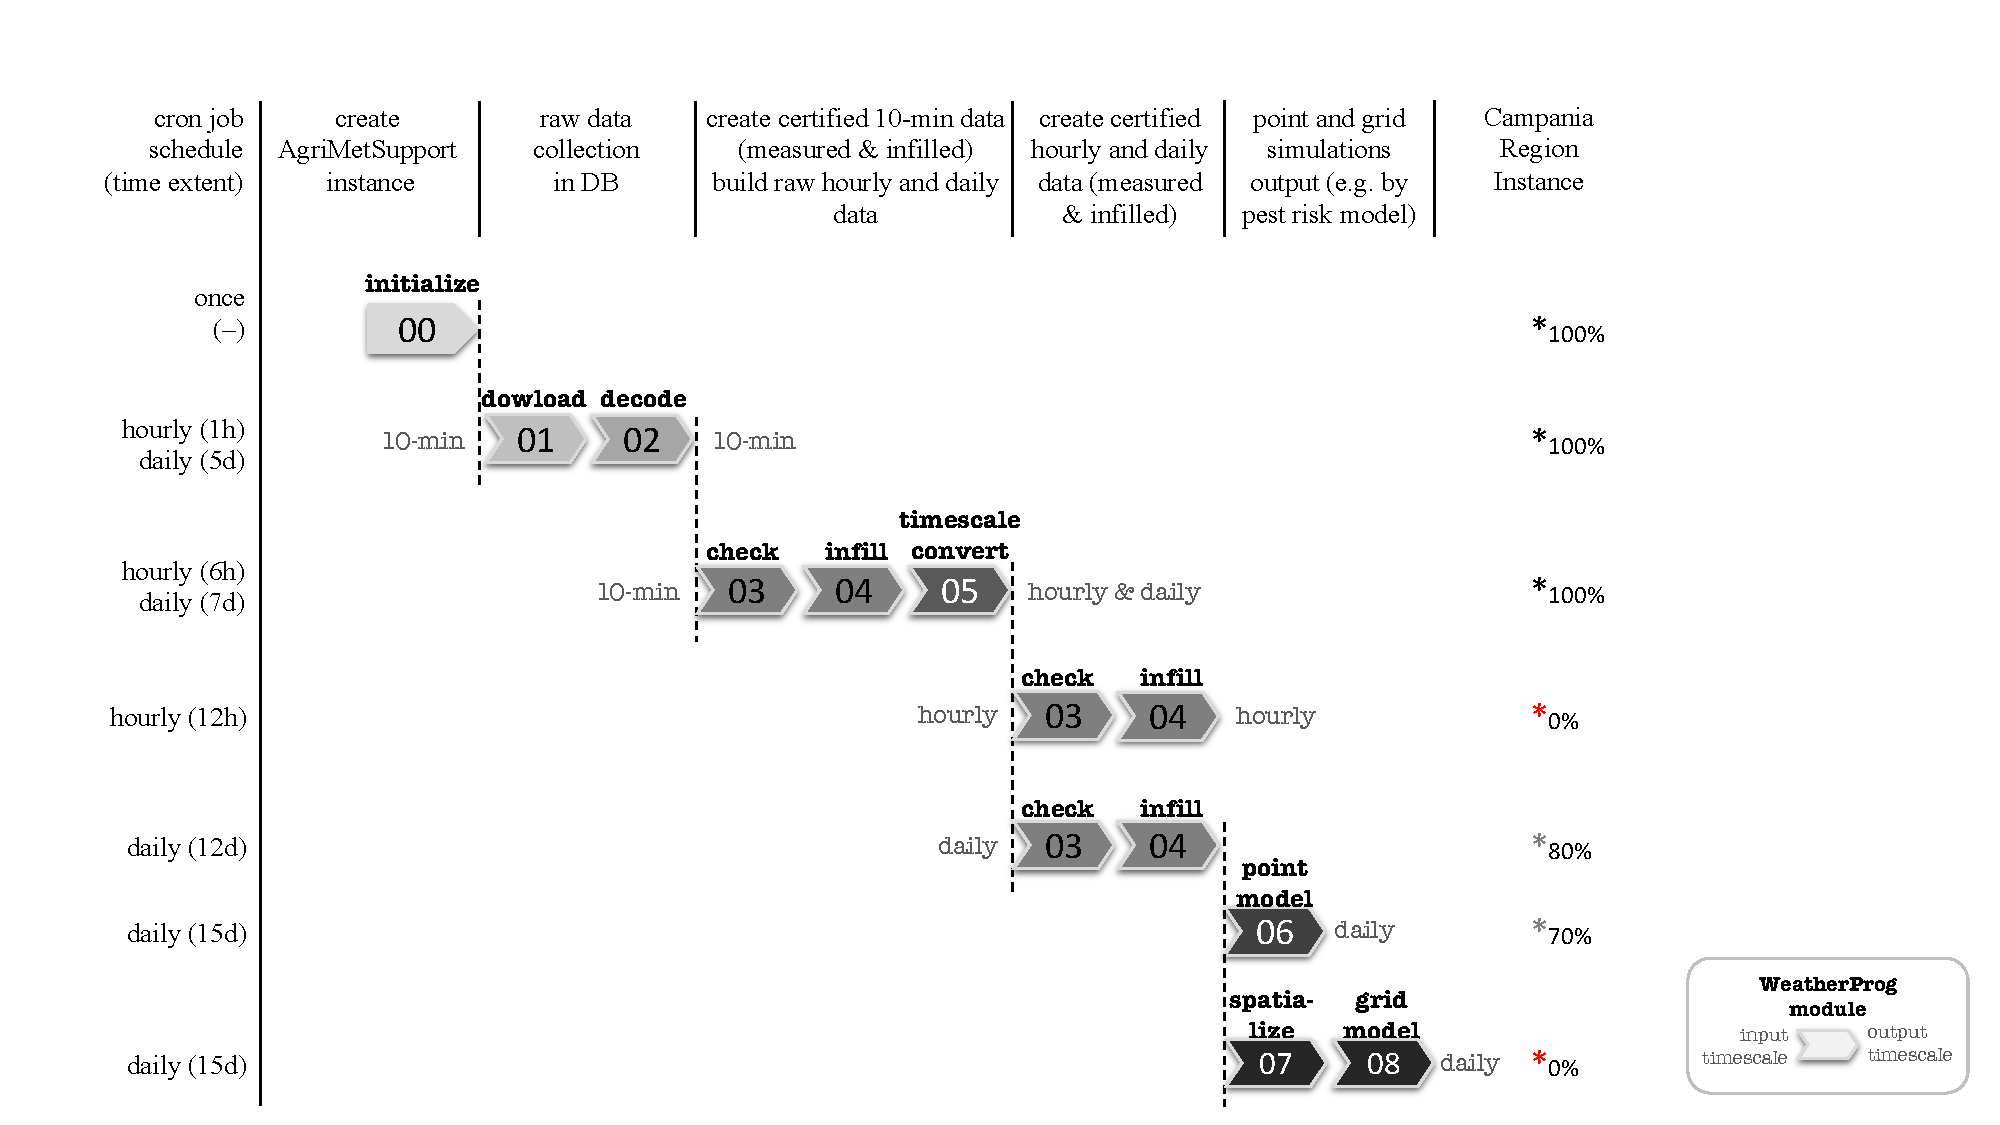
\includegraphics[scale=.4]{figures/WeatherProg_fig.pdf}
	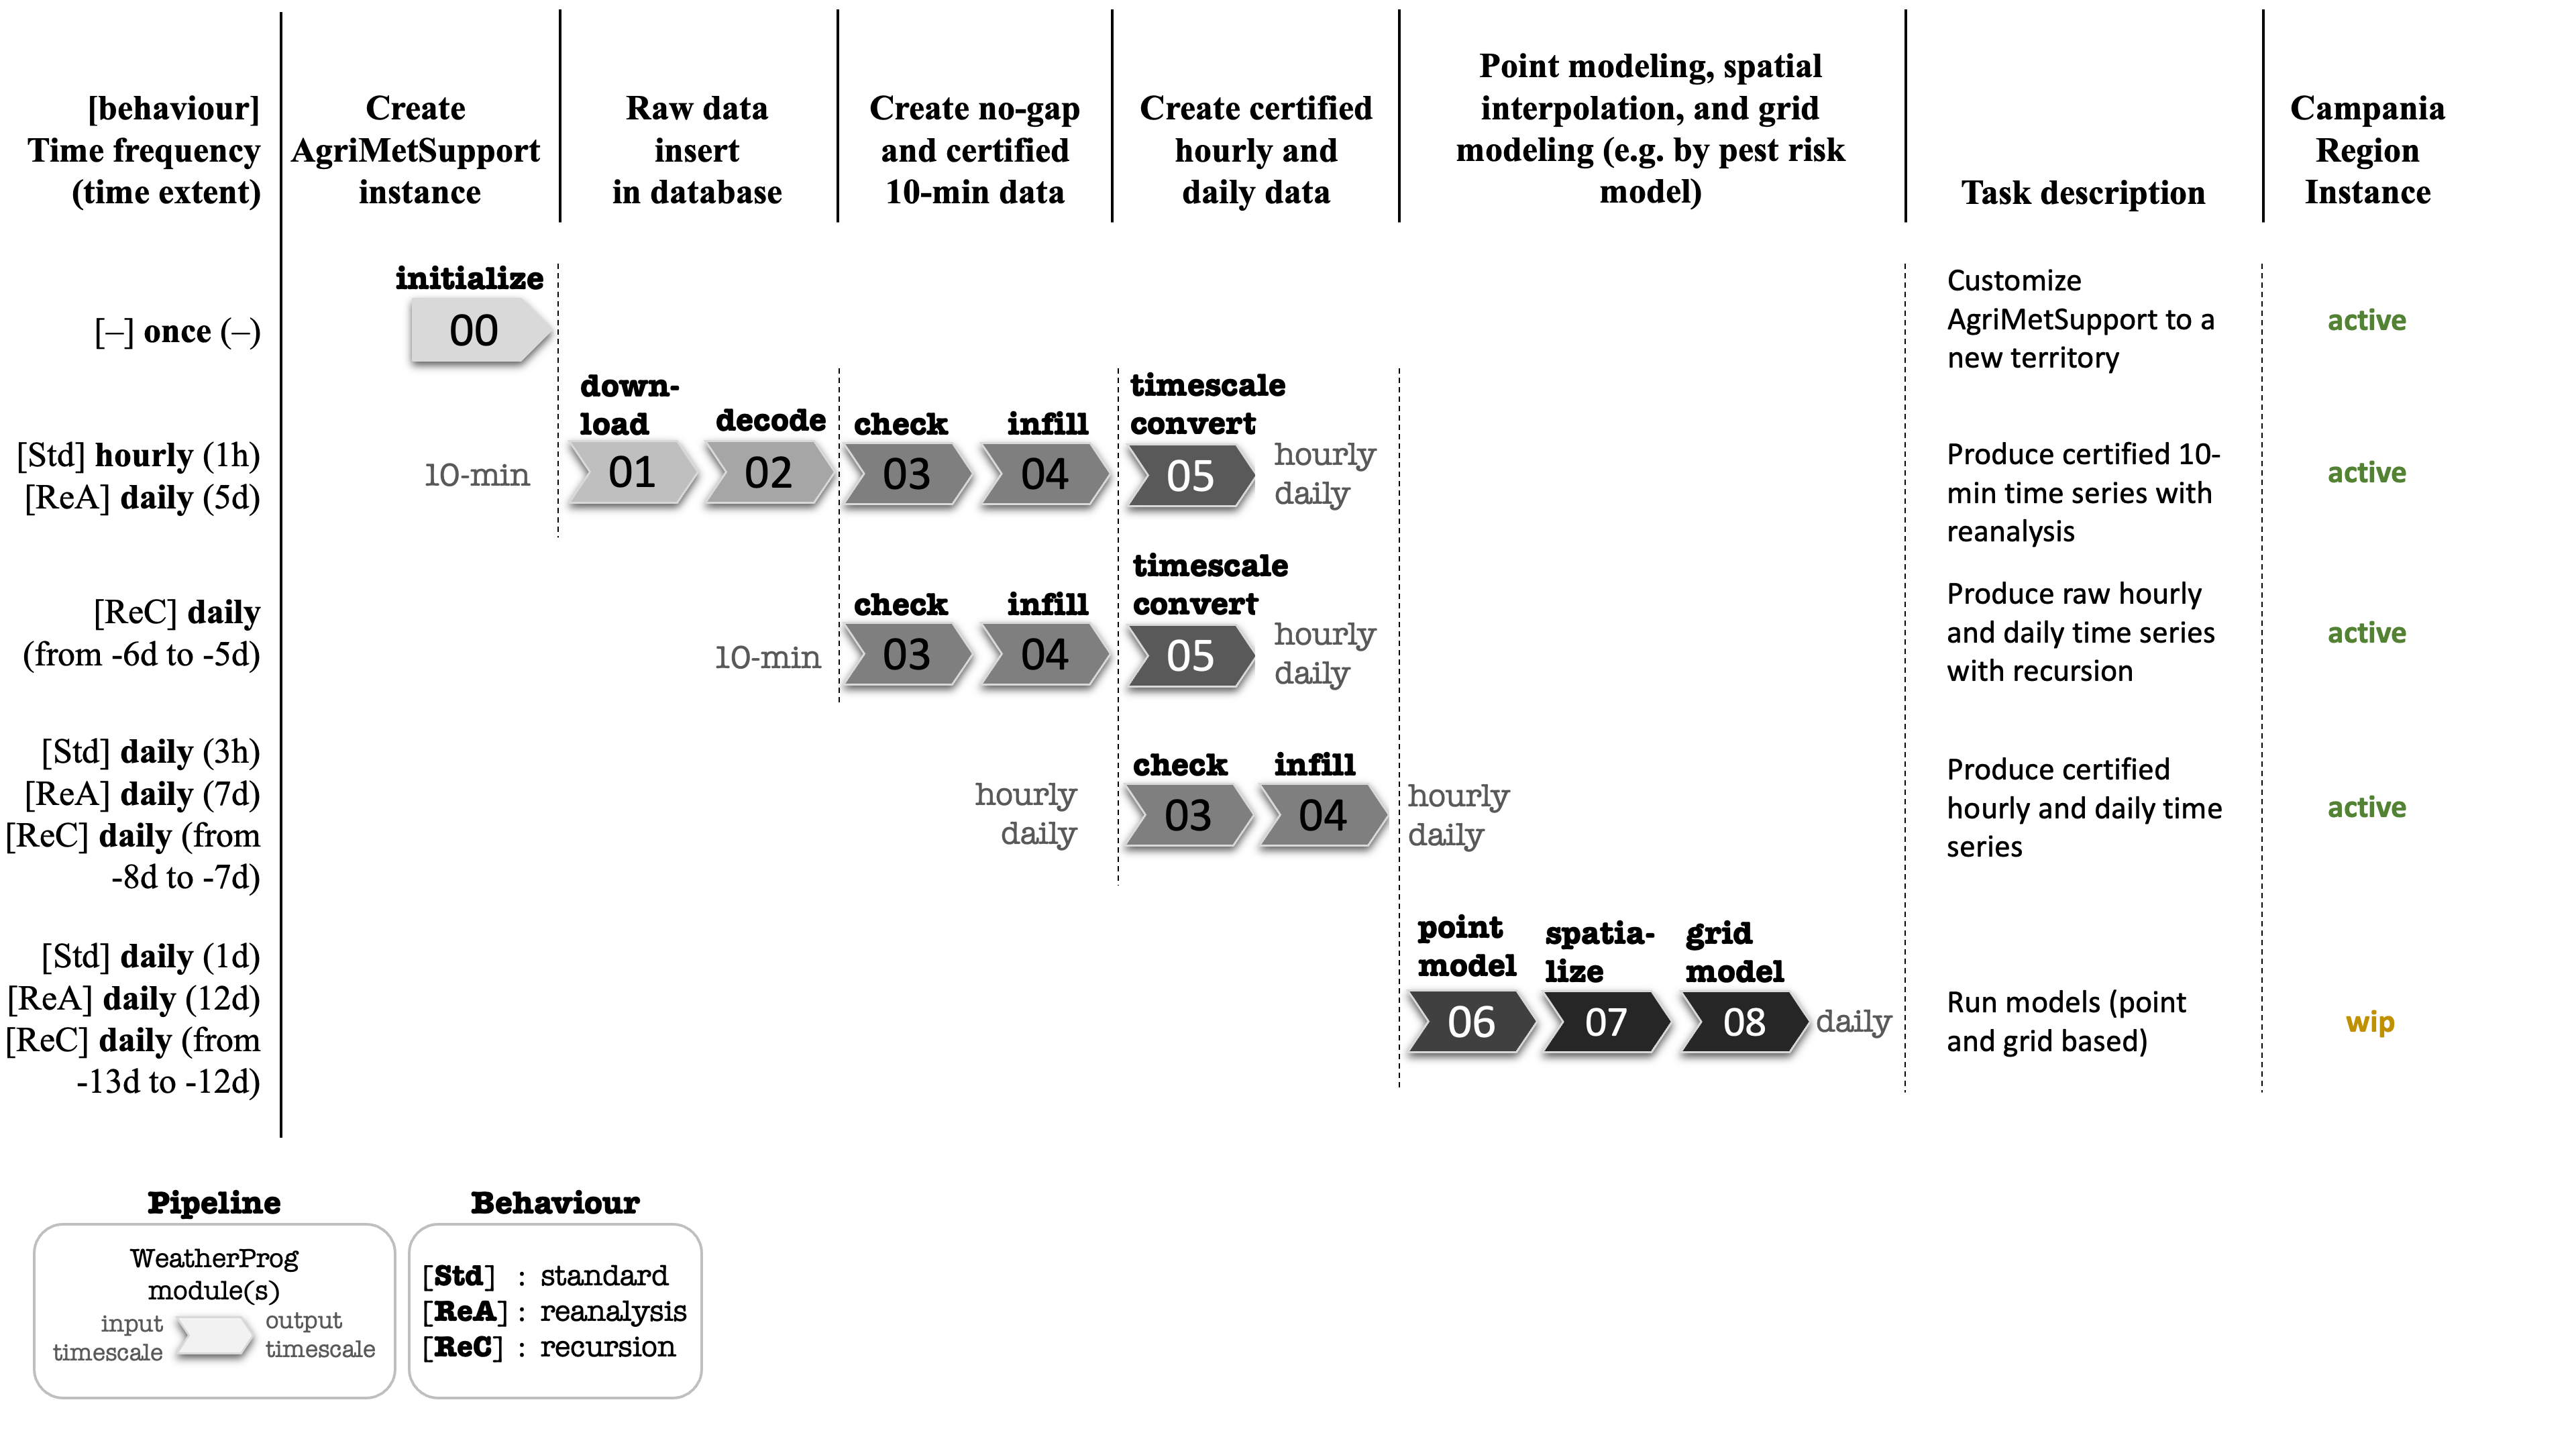
\includegraphics[scale=.6, angle=90, trim=0 2cm 7cm 2cm]{figures/WeatherProg-schedule-fig-v2.png}
	\caption{ \textbf{\DIFaddFL{NOTES: add }\textit{\DIFaddFL{hourly day}} \DIFaddFL{as input for point model; modify }\textit{\DIFaddFL{daily}} \DIFaddFL{output of grid model as }\textit{\DIFaddFL{hourly day}}\DIFaddFL{, this way it'll become compliant with figures `\mbox{%DIFAUXCMD
\cref{Box01:WeatherProg_Operations} }\hskip0pt%DIFAUXCMD
and \mbox{%DIFAUXCMD
\cref{Fig:WeatherProg}}\hskip0pt%DIFAUXCMD
; use always a negative value for "time extent" in the pipeline names because I use both + and - and it is not correct.}}\DIFaddFL{.
    WeatherProg job schedule for air temperature in a typical Agri\-Met\-Support instance.
    Each row of the schedule is a pipeline and a total of 10 pipelines are shown.
    Standard, reanalysis and recursive pipelines are orchestrated to build homogeneous and complete agrometeorological (point and grid) database.}}
	\label{Fig:weatherprog:calls}
\end{figure}
\DIFaddend In \cref{Fig:weatherprog:calls} a typical running schedule for air temperature is depicted, providing a reference to the specific case study of this work (i.e. Campania Region instance).
The schedule is composed of pipelines (each row in first column of Figure \ref{Fig:weatherprog:calls}) having different scopes which are orchestrated row-wise to manage all the basic and derived information required by \DIFdelbegin \DIFdel{AgriMetSupport}\DIFdelend \DIFaddbegin \DIFadd{Agri\-Met\-Support}\DIFaddend .
The WeatherProg modules are the fundamental bricks used in the composition of schedules.
The key schedule parameters are the time scale of the target agrometeorological variable (e.g. 10 minutes), the pipeline execution frequency (e.g. every day) and the time domain extent (last 5 days) tackled by each pipeline run (first column of Figure \ref{Fig:weatherprog:calls}).
It means that the pipeline is executed every hour or every 3 days and works on a temporal window active only within the defined time extent, for instance from 6 days (-6d) to 5 days (-5d) before execution time.

This flexible configuration is further enhanced by the behaviour of the pipeline, since the schedule can have reanalysis and recursive pipelines in addition to a standard one (with a total of 10 rows, resulting in a corresponding number of pipelines in Figure \ref{Fig:weatherprog:calls}).

A reanalysis pipeline builds a progressively updated version of quality controlled and infilled data (ReA in Figure \ref{Fig:weatherprog:calls}).
To cite an instance, the persistence control type strictly depends on reanalysis to write a meaningful flag, since only adjacent records in the time series that have already passed logic and continuity control types (that is only auxiliary data of good quality) can contribute. % to the quality control procedure.
As time passes by, more auxiliary measurements are available within the time window of WeatherProg modules in execution (both before and after the target time being checked). 
Until the last execution of the reanalysis, which happens when the moving window is out of range for a target time element, an updated version of both quality checked and infilled data is produced (data and flags are overwritten) while infilled data undergo a separate process and are not subjected to quality control.
At this point, the time element, which is out of range of the moving window after the last reanalysis run, undergoes the recursion run.
A recursion pipeline (ReC in Figure \ref{Fig:weatherprog:calls}) is in charge of performing a quality check including infilled data and eventually performing a new infill procedure for each missing or anomalous singleton.
From now on, the time series is stable till the time element targeted by the last recursion run.

\DIFdelbegin %DIFDELCMD < \begin{figure}
%DIFDELCMD < 	\centering %%%
%DIF <  trim=left bottom right top
	%DIF < 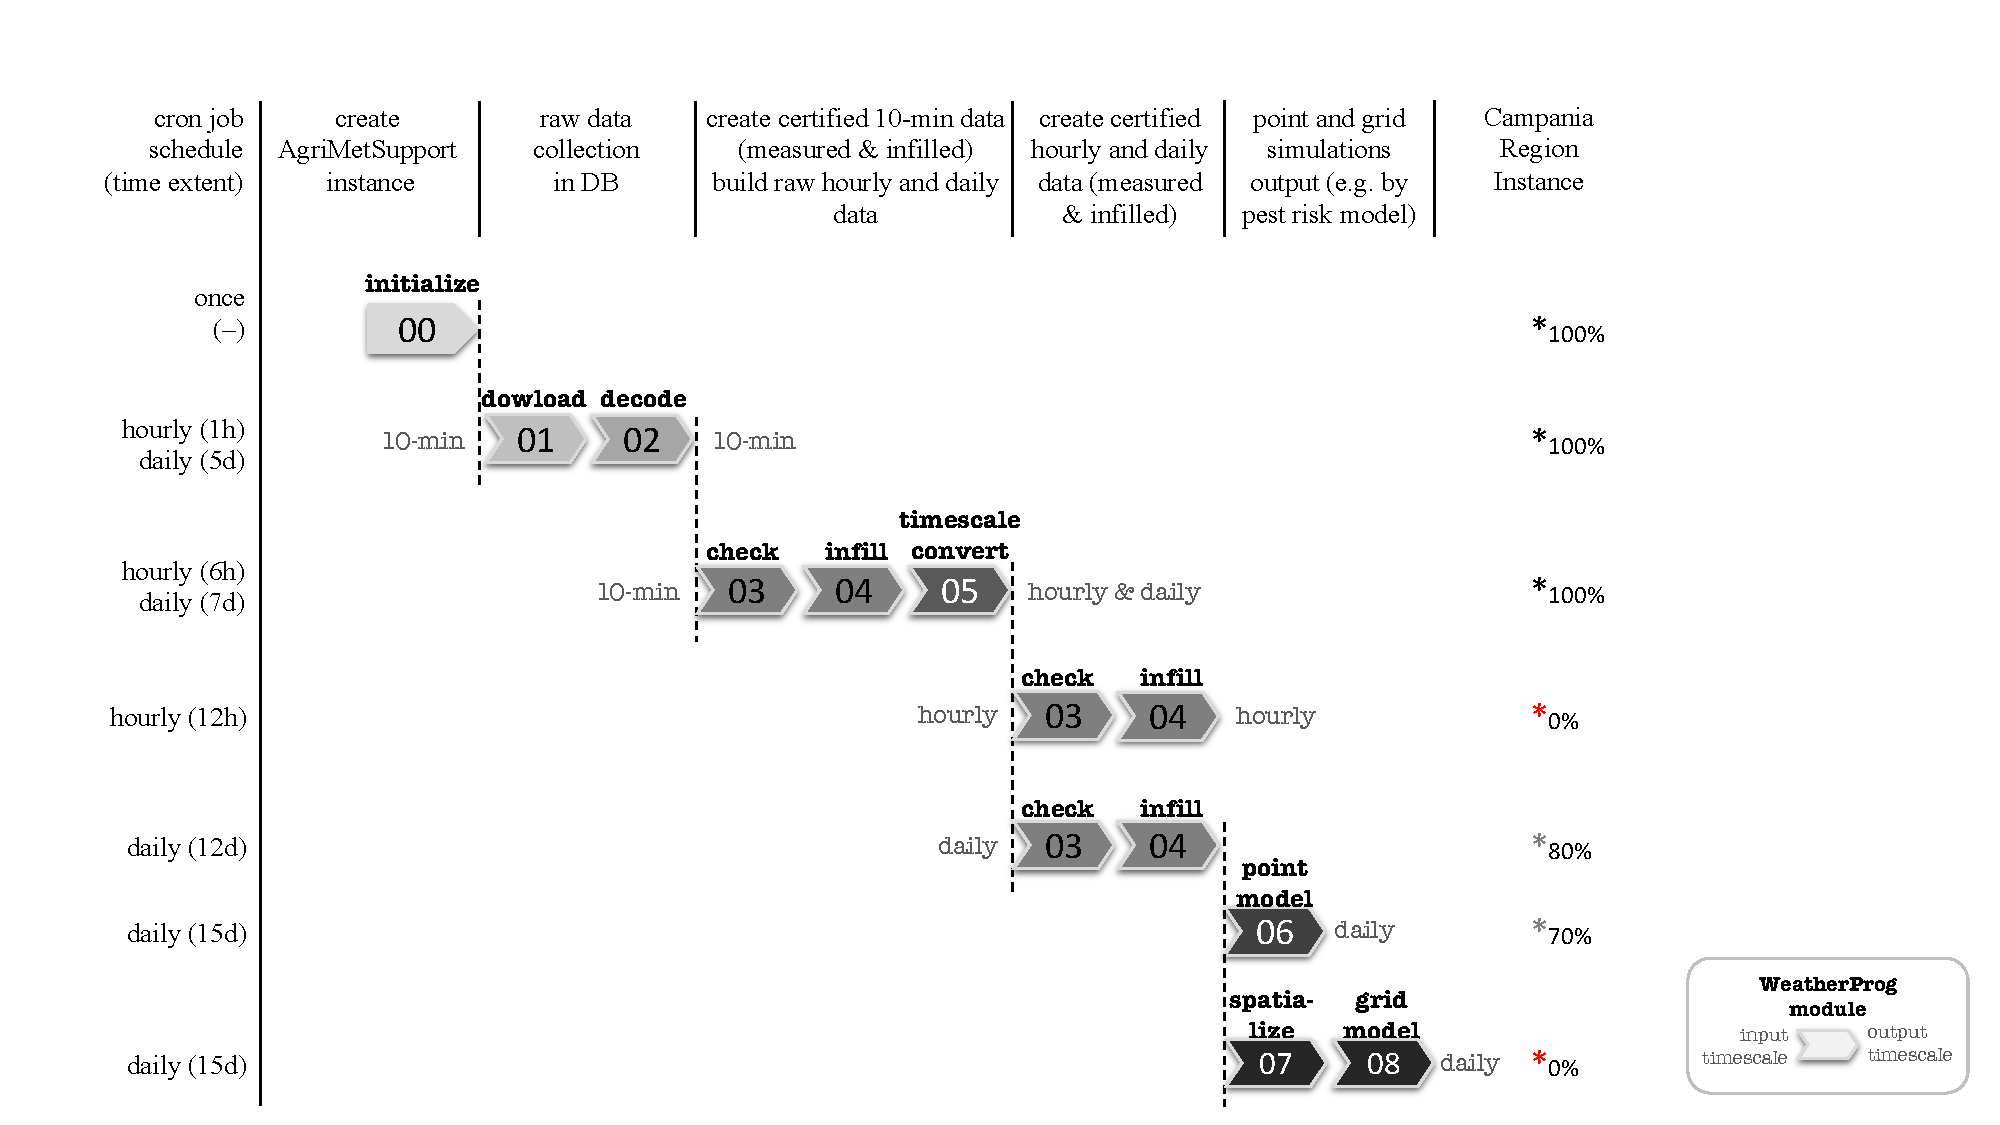
\includegraphics[scale=.4]{figures/WeatherProg_fig.pdf}
	%DIFDELCMD < 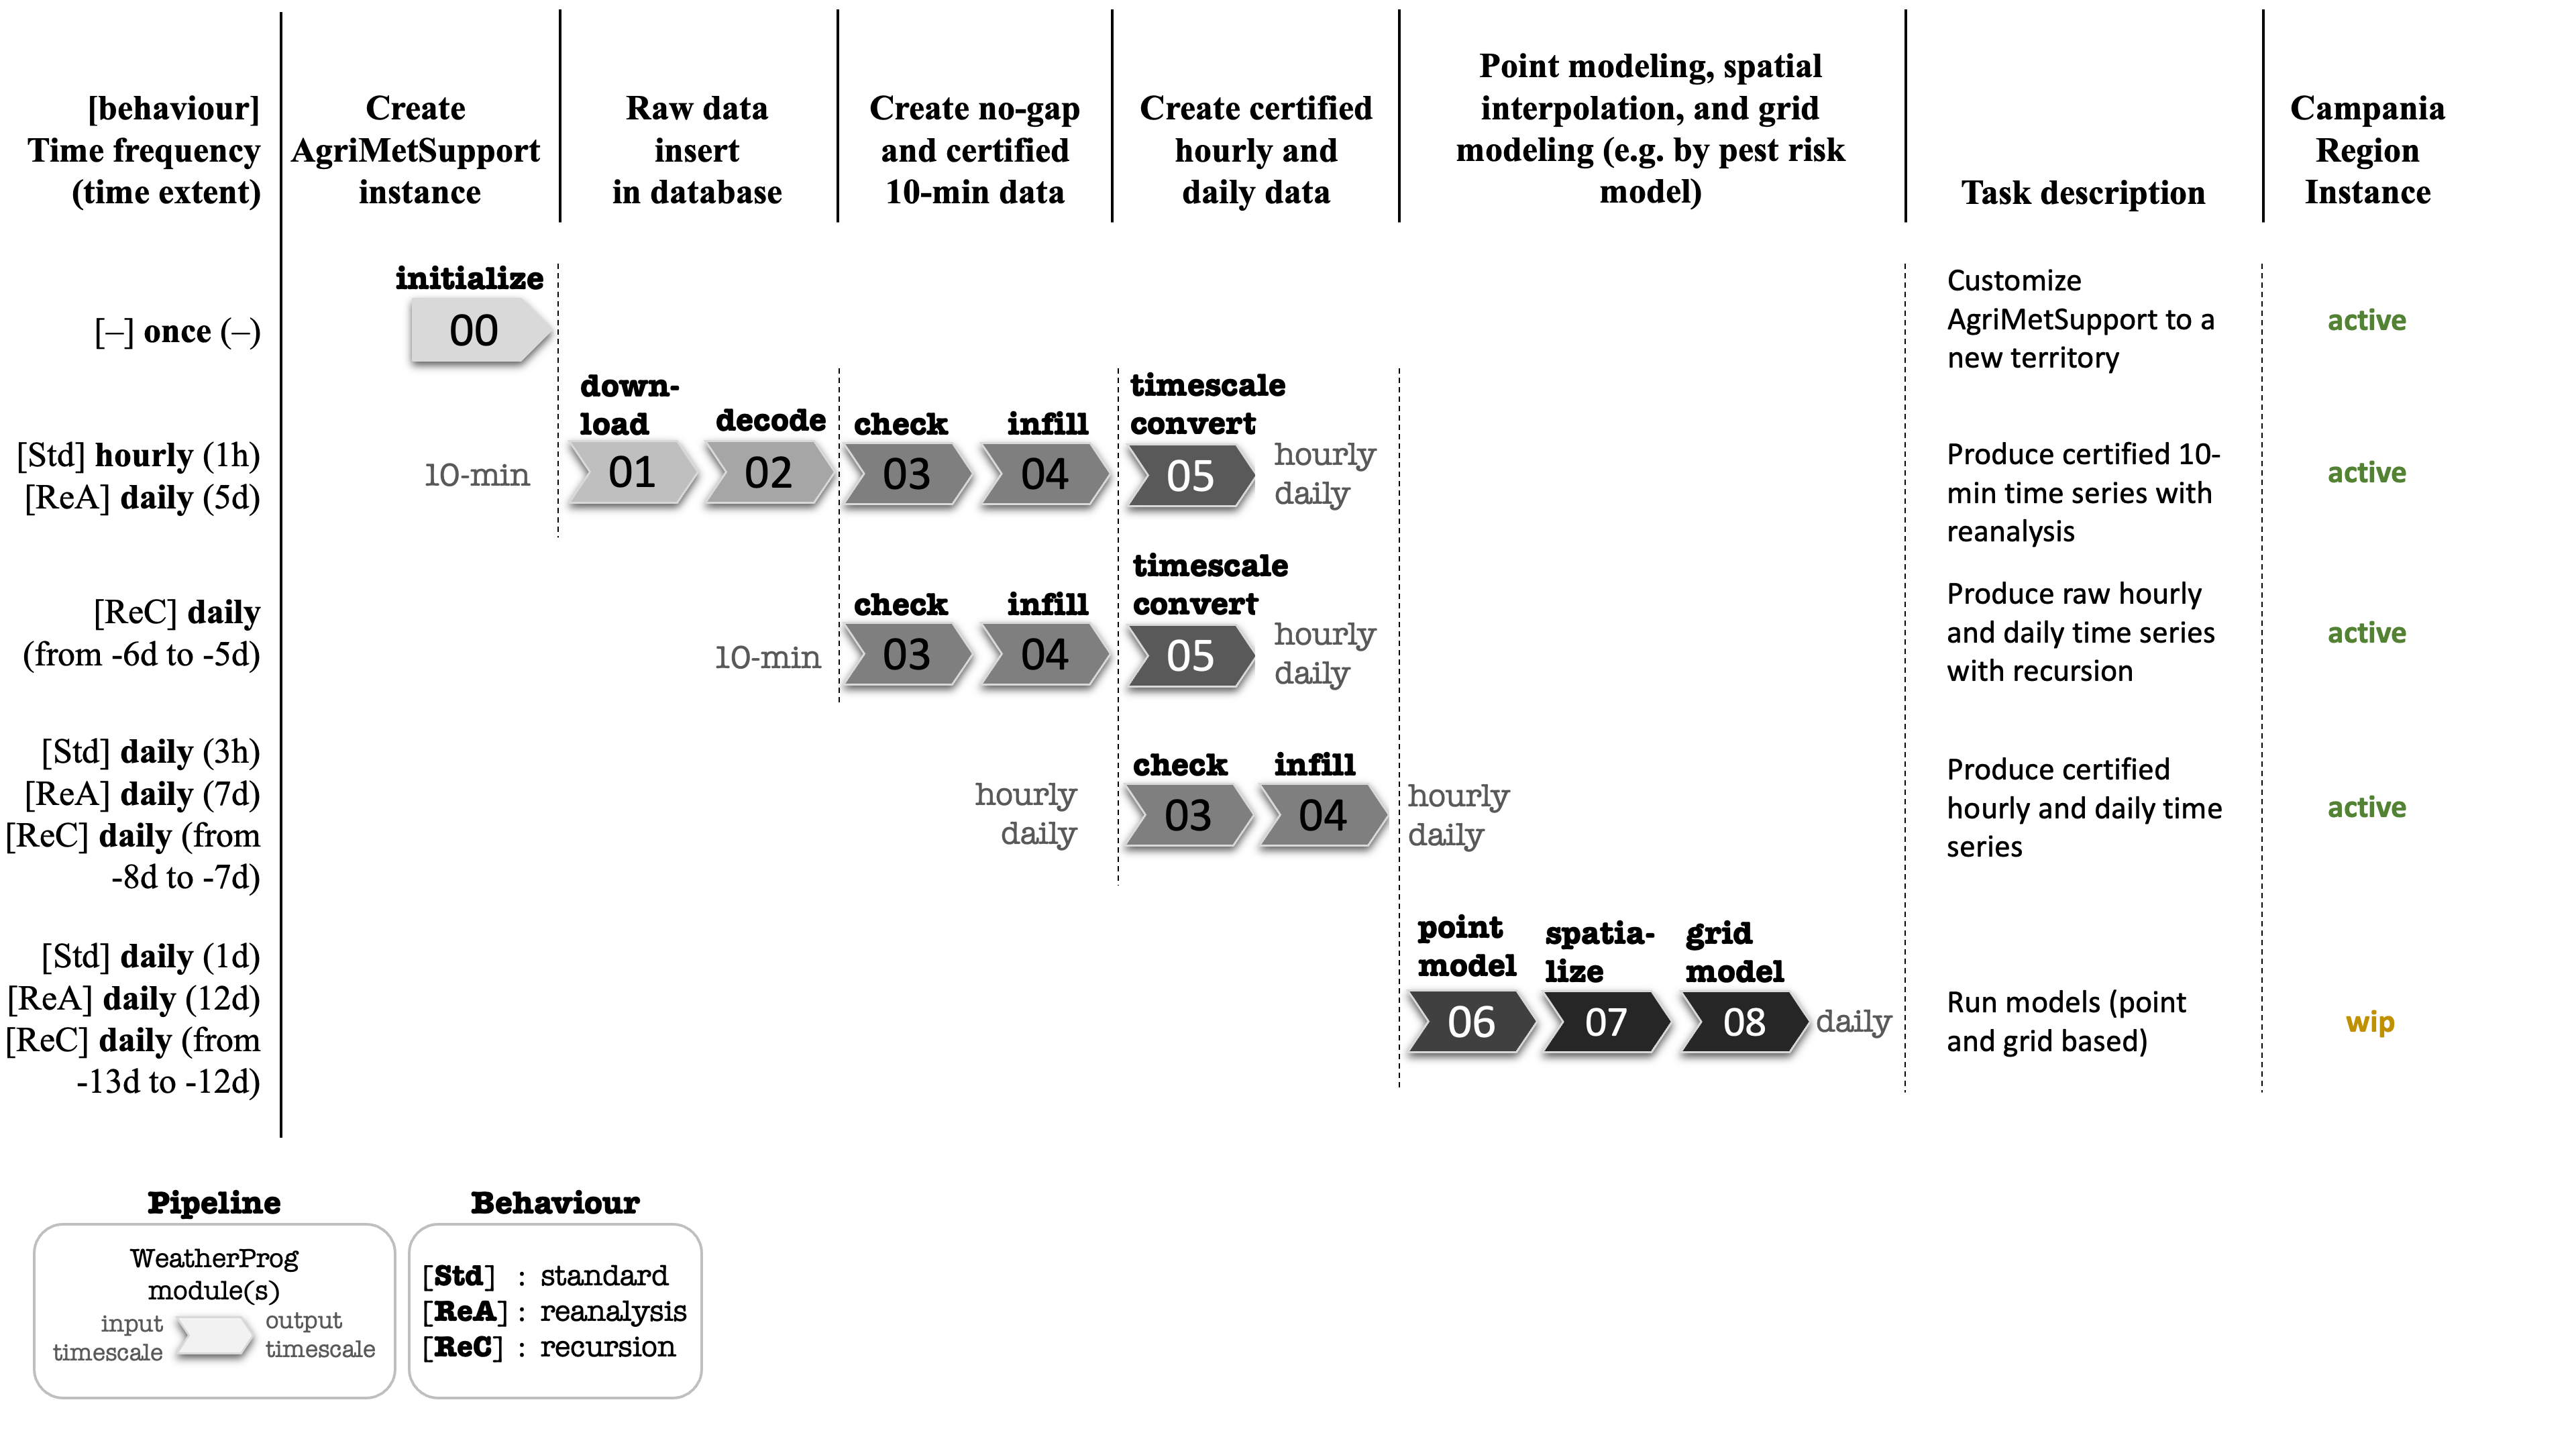
\includegraphics[scale=.6, angle=90, trim=0 2cm 7cm 2cm]{figures/WeatherProg-schedule-fig-v2.png}
%DIFDELCMD < 	%%%
%DIFDELCMD < \caption{%
{%DIFAUXCMD
\DIFdelFL{WeatherProg job schedule for air temperature in a typical AgriMetSupport instance.
 Each row of the schedule is a pipeline and a total of 10 pipelines are showed.
 Standard, reanalysis and recursive pipelines are orchestrated to build homogeneous and complete agrometeorological (point and grid) database.}}
	%DIFAUXCMD
%DIFDELCMD < \label{Fig:weatherprog:calls}
%DIFDELCMD < \end{figure}
%DIFDELCMD < 

%DIFDELCMD < %%%
\DIFdelend \section{Create qualified and certified data with no gaps} \label{sec:qck+fill}
%The deviation or switch was introduced in the 10-minutes pipeline tackling the daily run dedicated to the creation of no-gap and certified data, as depicted in \cref{Fig:weatherprog:calls} . \note{(MODIFY THE FIGURE TO ADD THE DEVIATION/SWITCH GRAPHICALLY))}.

\subsection{Quality control\DIFdelbegin \DIFdel{procedure}\DIFdelend } \label{sec:qcheck}
WeatherProg has a quality control module capable to managing data at 10 minutes, hourly and daily time scales.
The quality control can be of different types, such as range, continuity, persistence, climatological, spatial and temporal and not all quality control types are available neither at all time scales nor for all agrometeorological variables.
Possible flags for both any quality control type and the overall outcome are reported in \cref{tab:flagsSummary} with a short description for each flag.
\DIFdelbegin %DIFDELCMD < 

%DIFDELCMD < %%%
\DIFdel{When a new AgriMetSupport instance is created a new database is created too.
Agrometeorological 10-minutes data are inserted for the first time and they can span for a day, for a month, for a year or even for longer time periods.
This is an initial condition (see }\textit{\DIFdel{initialize}} %DIFAUXCMD
\DIFdel{in \mbox{%DIFAUXCMD
\cref{Fig:weatherprog:calls}}\hskip0pt%DIFAUXCMD
) in which all flags are switched to unchecked for all control types and to unprocessed for the overall outcome.
After the database is created with this first data ingest, WeatherProg is executed once carrying out a long-term run (LTR) on the whole available time series.
Taking as an example the schedule depicted in \mbox{%DIFAUXCMD
\cref{Fig:weatherprog:calls} }\hskip0pt%DIFAUXCMD
for air temperature, the LTR executes only the range control on the whole time series at first step and then a new LTR is executed adding the other control types step by step.
In the last step, the LTR executes the control types all together completing the initialization step.
Once the LTR writes all quality control flags, the high gear condition is met and WeatherProg can run the pipelines as outlined in the schedule of \mbox{%DIFAUXCMD
\cref{Fig:weatherprog:calls}}\hskip0pt%DIFAUXCMD
.
}%DIFDELCMD < 

%DIFDELCMD < %%%
\DIFdel{For simplicity, an overview of the quality control logic is presented only at the 10 minutes time scale for air temperature (\mbox{%DIFAUXCMD
\cref{tab:qcheck_m10_airT}}\hskip0pt%DIFAUXCMD
) both in this section and in section \ref{sec:QcheckValidation} where the quality control procedure will be validated.
There is an implementation logic based on 15 different combinations of four quality control types, namely range, continuity, persistence and spatial.
Each combination or row shown in \mbox{%DIFAUXCMD
\cref{tab:qcheck_m10_airT} }\hskip0pt%DIFAUXCMD
can be reached only if all previous combinations are not satisfied.
The sequence of combinations on rows depends on the absolute and relative weight given to each control type.
Let's provide few examples for any given datum.
If the range control type returns a wrong flag it is unnecessary to check any other control type and the overall quality control procedure has an outcome flag equal to wrong (ID=3 in \mbox{%DIFAUXCMD
\cref{tab:qcheck_m10_airT}}\hskip0pt%DIFAUXCMD
).
Further, if range is correct and continuity is wrong it is unnecessary to consider the flags for persistence and spatial control types and the overall quality control procedure has an outcome flag equal to wrong again (ID=8 in \mbox{%DIFAUXCMD
\cref{tab:qcheck_m10_airT}}\hskip0pt%DIFAUXCMD
).
Conversely, if range is correct and continuity is dubious than the spatial flag is relevant to get an overall outcome correct (ID=9 in \mbox{%DIFAUXCMD
\cref{tab:qcheck_m10_airT}}\hskip0pt%DIFAUXCMD
), wrong (ID=10 in \mbox{%DIFAUXCMD
\cref{tab:qcheck_m10_airT}}\hskip0pt%DIFAUXCMD
) or even dubious (ID=11 in \mbox{%DIFAUXCMD
\cref{tab:qcheck_m10_airT}}\hskip0pt%DIFAUXCMD
) according to the continuity status of other stations in the spatial neighbourhood of the station being processed.
In general, the implemented logic forces to reduce the probability of dubious flags since a dubious singleton is not discarded until either evidence or a human sets it as either correct or wrong.
}%DIFDELCMD < 

%DIFDELCMD < %%%
%DIF < The description of flags for the outcome of the quality control procedure can be found in %\cref{tab:qcheckOutcomeFlagsSummary}.
%DIF < \note{I would fuse \cref{tab:flagsSummary} and \cref{tab:qcheckOutcomeFlagsSummary}}.
%DIFDELCMD < 

%DIFDELCMD < %%%
\DIFdelend \begin{table}[]
    \begin{scriptsize}
    \centering
    \begin{tabular}{r r l p{7cm}}
    % \multicolumn{2}{c}{Blablabla} \\
    \hline
    Control element & Flag & Abbreviation & Description \\
    \hline
	Control types & UNCHECKED     & UC & The quality control type has not been applied yet. Either this measurement has not undergone quality control at all yet, or this type was disabled.\\
	& CORRECT       & C  & This measurement appears to be correct according to this quality control type. \\
	& DUBIOUS       & D  & The quality control type has completed, but it cannot decide neither for correctness nor for wrongness. \\
	& AUXMISSING    & AM & The quality control type cannot complete, due to the lack of required auxiliary data. \\
	& AUXUNRELIABLE & AU & The quality control type cannot complete, because the required auxiliary data are available but they have not passed the quality control procedure themselves yet. \\
	& WRONG         & W  & This measurement appears to be wrong according to this quality control type. \\

    \hline

	Control procedure & UNPROCESSED & UP & This measurement has not undergone quality control at all yet.\\
	& CORRECT     & C  & This measurement is deemed correct by the quality control procedure.\\
	& DUBIOUS     & D  & This measurement is suspicious, but the quality control procedure cannot decide neither for correctness nor for wrongness. A knowledge-based human checking is required. \\
	& UNDECIDED   & UD & The measurement has been subject to the quality control procedure, but there is not sufficient ground yet to decide either for correctness or for wrongness. Reanalysis runs may have the additional information required to solve the indecision.\\
	& WRONG       & W  & This measurement is deemed not correct by the quality control procedure.\\
    \hline    
    \end{tabular}
    \caption{Flags used in any quality control type (range, continuity, persistence, climatological, spatial, temporal) and possible outcome status of the overall quality control procedure.}
    \label{tab:flagsSummary}
    \end{scriptsize}
\end{table}

\DIFdelbegin %DIFDELCMD < \begin{table}[]
%DIFDELCMD <     %%%
\DIFdelendFL \DIFaddbeginFL \DIFaddFL{When a new Agri\-Met\-Support instance is created a new point database is created too.
Agrometeorological 10-minutes data are inserted for the first time and they can span for a day, for a month, for a year or even for longer time periods.
This is an initial condition (see }\textit{\DIFaddFL{initialize}} \DIFaddFL{in \mbox{%DIFAUXCMD
\cref{Fig:weatherprog:calls}}\hskip0pt%DIFAUXCMD
) in which all flags are switched to unchecked for all control types and to unprocessed for the overall outcome.
After the database is created with this first data ingest, WeatherProg is executed once carrying out a long-term run (LTR) on the whole available time series.
Taking as an example the schedule depicted in \mbox{%DIFAUXCMD
\cref{Fig:weatherprog:calls} }\hskip0pt%DIFAUXCMD
for air temperature, the LTR first executes the range control on the entire time series before progressively applying the other control types, one at a time. 
This stepwise approach is necessary because the quality of the data affects the control procedure itself: in order to apply more refined checks, we need a reliable initial assessment of data validity.
By starting with range control, we establish a preliminary quality check, which then allows subsequent controls to refine the data evaluation without being misled by poor-quality inputs.
In the last initialization step, the LTR executes all control types together, ensuring that the initially ingested data has been fully checked and is actually usable for the control procedure itself.
Once the LTR writes all quality control flags, the high gear condition is met and WeatherProg can run the pipelines as outlined in the schedule of \mbox{%DIFAUXCMD
\cref{Fig:weatherprog:calls}}\hskip0pt%DIFAUXCMD
.
}

\begin{table}[h]
    \DIFaddendFL \begin{scriptsize}
    \centering
    \begin{tabular}{l l l l l l l}
        \hline
      \DIFdelbeginFL \DIFdelFL{ID }\DIFdelendFL \DIFaddbeginFL \DIFaddFL{Rule }\DIFaddendFL & Logical  \DIFdelbeginFL \DIFdelFL{Operator }\DIFdelendFL & Range & Continuity & Persistence      & Spatial      & Outcome \\
        \DIFaddbeginFL \DIFaddFL{ID }& \DIFaddFL{Operator }&       &            &                  &              &         \\
        \DIFaddendFL \hline
        1  & or               & UC    & UC         & UC               & UC           & UP \\
        2  & and              & C     & C          & C                & C            & C  \\
        3  & and              & W     & any        & any              & any          & W  \\
        4  & and              & C     & any        & W                & any          & W  \\
        5  & and              & C     & AU | AM    & AU | AM          & AU | AM      & UD \\
        6  & and              & C     & C          & C | AU | AM      & C | D        & C  \\
        7  & and              & C     & C          & C | AU | AM      & W            & D  \\
        8  & and              & C     & W          & any              & any          & W  \\
        %8  & and              & C     & W          & C | AU | AM      & D | W        & W  \\
        9  & and              & C     & D | W      & C | AU | AM      & C            & C  \\
        10 & and              & C     & D          & C | AU | AM      & W            & W  \\
        11 & and              & C     & D          & C | AU | AM      & D            & D  \\
        12 & and              & C     & W          & C | UC | AU | AM & UC | AU | AM & W  \\
        13 & and              & C     & D          & C | UC | AU | AM & UC | AU | AM & D  \\
        14 & and              & C     & C          & C | UC | AU | AM & UC | AU | AM & C  \\
        15 & or               & C     & AU | AM    & AU | AM          & AU | AM      & UD \\
        \hline
    \end{tabular}
    \end{scriptsize}
    \caption{\DIFdelbeginFL \DIFdelFL{Logic of }\DIFdelendFL \DIFaddbeginFL \DIFaddFL{Logic-based conditions for }\DIFaddendFL the quality control \DIFdelbeginFL \DIFdelFL{procedure and outcomes implemented for the }\DIFdelendFL \DIFaddbeginFL \DIFaddFL{of }\DIFaddendFL air temperature at \DIFdelbeginFL \DIFdelFL{the 10 minutes }\DIFdelendFL \DIFaddbeginFL \DIFaddFL{a 10-minute }\DIFaddendFL time scale.
    Flags \DIFdelbeginFL \DIFdelFL{are described in \mbox{%DIFAUXCMD
\cref{tab:flagsSummary} }\hskip0pt%DIFAUXCMD
}\DIFdelendFL for both \DIFdelbeginFL \DIFdelFL{the }\DIFdelendFL quality control types and \DIFdelbeginFL \DIFdelFL{the }\DIFdelendFL final outcome status \DIFaddbeginFL \DIFaddFL{are described in \mbox{%DIFAUXCMD
\cref{tab:flagsSummary}}\hskip0pt%DIFAUXCMD
}\DIFaddendFL .
    \DIFdelbeginFL \DIFdelFL{More }\DIFdelendFL \DIFaddbeginFL \DIFaddFL{Multiple }\DIFaddendFL flags in the same cell are aggregated using the \textit{or} logical operator.
    For instance, persistence can be either AU or AM \DIFdelbeginFL \DIFdelFL{at }\DIFdelendFL \DIFaddbeginFL \DIFaddFL{for }\DIFaddendFL ID = 5. }
    \label{tab:qcheck_m10_airT}
\end{table}
\DIFaddbegin \DIFadd{An overview of the quality control logic is presented at the 10 minutes time scale for air temperature (\mbox{%DIFAUXCMD
\cref{tab:qcheck_m10_airT}}\hskip0pt%DIFAUXCMD
).
There is an implementation logic based on 15 different rules, each defined by a combination of four quality control types: range, continuity, persistence, and spatial.
Each rule is represented in \mbox{%DIFAUXCMD
\cref{tab:qcheck_m10_airT} }\hskip0pt%DIFAUXCMD
as a row and can be applied only if all preceding rules are not met.
The order or priority of the rules depends on the absolute and relative weight assigned to each control type and their combination.
Let's provide few examples for any given datum.
The first rule sets an unprocessed (UP) flag if any control type was not carried out (unchecked flag or UC).
The second rule ensures that the datum flag is set to correct if all control types have a correct flag.
If the range control type returns a wrong flag it is unnecessary to check any other control type and the overall quality control procedure has an outcome flag equal to wrong (rule 3 in \mbox{%DIFAUXCMD
\cref{tab:qcheck_m10_airT}}\hskip0pt%DIFAUXCMD
).
Further, if range is correct and continuity is wrong it is unnecessary to consider the flags for persistence and spatial control types and the overall quality control procedure has an outcome flag equal to wrong again (rule 8 in \mbox{%DIFAUXCMD
\cref{tab:qcheck_m10_airT}}\hskip0pt%DIFAUXCMD
).
Conversely, if range is correct and continuity is dubious than the spatial flag is relevant to get an overall outcome correct (rule 9 in \mbox{%DIFAUXCMD
\cref{tab:qcheck_m10_airT}}\hskip0pt%DIFAUXCMD
), wrong (rule 10 in \mbox{%DIFAUXCMD
\cref{tab:qcheck_m10_airT}}\hskip0pt%DIFAUXCMD
) or even dubious (rule 11 in \mbox{%DIFAUXCMD
\cref{tab:qcheck_m10_airT}}\hskip0pt%DIFAUXCMD
) according to the continuity status of other stations in the spatial neighbourhood of the station being processed.
In general, the implemented logic minimizes the likelihood of assigning dubious flags, as a dubious singleton is not discarded until either new evidence emerges or a human intervention classifies it as correct or wrong. 
Since quality control is performed on a moving window, the best assessment of a target value is achieved only when it is centered in the window and all auxiliary measurements within the window have successfully passed quality control. 
This is the reason why, for example, in \mbox{%DIFAUXCMD
\cref{Fig:weatherprog:calls}}\hskip0pt%DIFAUXCMD
, there is a pipeline dedicated to the reanalysis of 10-minute data, which is run once per day and involves the data of the last 5 days (the pipeline label is '}[\DIFadd{ReA}] \DIFadd{daily (-5d)').
However, this duration (5 days) does not correspond to the window length used in quality control.
For instance, if the window length for the quality control of target 10-minute measurements is $\pm100$ time steps, then it is plausible that measurements from day -5 to -3 have the best conditions for evaluation.
}\DIFaddend 

%DIF > The description of flags for the outcome of the quality control procedure can be found in %\cref{tab:qcheckOutcomeFlagsSummary}.
%DIF > \note{I would fuse \cref{tab:flagsSummary} and \cref{tab:qcheckOutcomeFlagsSummary}}.
\DIFaddbegin 


\DIFaddend \subsection{Gap-filling\DIFdelbegin \DIFdel{procedure}\DIFdelend } \label{sec:infill}
%Anomalies and missing data are all flagged to be %interpolated by means of an automatic linear regression procedure.
%infilled in order to get complete and homogeneous time series.
%Different methods are available such as a deterministic approach based on moving average with a growing kernel, or a statistical method approach using a stepwise multilinear regression using other stations after an iterative optimization step to properly select the time series length and the regression covariates.

WeatherProg has a module equipped with basic gap-filling methods which are dedicated to filling anomalies and data gaps.
\DIFdelbegin \DIFdel{For the purpose of this paper, }\DIFdelend \DIFaddbegin \DIFadd{In the AgriMetSupport instance for Campania region }\DIFaddend the infilling method \DIFdelbegin \DIFdel{based on }\DIFdelend \DIFaddbegin \DIFadd{was configured to use the }\DIFaddend stepwise multiple linear regression (MLR)\DIFdelbegin \DIFdel{was used in order to allow for a validation analysis (see \mbox{%DIFAUXCMD
\cref{sec:QcheckValidation}}\hskip0pt%DIFAUXCMD
)}\DIFdelend .
The MLR methods starts with the selection of all gaps and anomalies for any station within a given \DIFaddbegin \DIFadd{the }\DIFaddend interval of time \DIFaddbegin \DIFadd{defined by the pipeline}\DIFaddend .
Then, for each datum to be infilled an optimisation block is executed iteratively on different time series lengths and on different numbers of regression covariates (i.e. the other stations used as independent variables in MLR).
Amongst the several regression models built for a missing or anomalous datum, the model characterised by the lowest RMSE is selected to predict the infilled value for that station in that date and time.
%The procedure is capable of dealing with all the anomalies and gaps while for any station found in a reference time interval.
Generally, the infill module avoids the selection of singletons that couldn't pass the quality check procedure. 
It means that data being potentially used as auxiliary but having flags different from correct or dubious are discarded from covariates.

\section{Case study: \DIFdelbegin \DIFdel{AgriMetSupport }\DIFdelend \DIFaddbegin \DIFadd{Agri\-Met\-Support }\DIFaddend at work in Campania Region} \label{sec:casestudy}

An \DIFdelbegin \DIFdel{AgriMetSupport }\DIFdelend \DIFaddbegin \DIFadd{Agri\-Met\-Support }\DIFaddend instance was tailored to the requirements of the Campania Region during the period 2016-2022.
%\review{ [...put here more text about the initialisation, also recalled in the end of Introduction.] }
This is of particular relevance considering huge limitations and constraints therein present.
Important limitations are the eco-environmental complexity of the study area, the scarcity of stations and the lack of long term time series for any station.
Other constraints are the urgent need for monitoring and sharing agrometeorological data in the regional territory %(highlight the important step forward thanks to our GCI)
and the urgent need for a system to assist the production of bulletins to help mitigate the effects of alien or autochthonous plant pests.

\subsection{Study area}\label{sec:StudyArea}
\DIFdelbegin \DIFdel{Located in southern }\DIFdelend \DIFaddbegin \DIFadd{The Campania region is located in the South of }\DIFaddend Italy between \ang{13;45;}E, \ang{15;49;}E, \ang{39;59;}N and \ang{41;31;}N,  \DIFdelbegin \DIFdel{Campania is the third most populated region of the Country, but due to its }\DIFdelend %DIF > is the third most populated region of the Country, but due to its 
\DIFaddbegin \DIFadd{featuring a long coastline along the Mediterranean Sea, and has an }\DIFaddend extension of about \SI{13600}{\metre\squared}\DIFdelbegin \DIFdel{, it is the most densely populated region of Italy. Its inland is occupied by the Apennine Mountains, oriented roughly NW-SE, whereas the Sele and Campana plains border the coast.
The Sele plain is named after the river which traverse it, while the Campana plain is traversed by the Volturno river.
Nevertheless, the }\DIFdelend \DIFaddbegin \DIFadd{. %DIF > , it is the most densely populated region of Italy.
%DIF > Its inland is occupied by the Apennine Mountains, oriented roughly NW-SE, whereas the Sele and Campana plains border the coast.
%DIF > The Sele plain is named after the river which traverse it, while the Campana plain is traversed by the Volturno river.
%DIF > Nevertheless, 
The }\DIFaddend majority of the regional territory is hilly, for the 50\% of the territory, against the 35\% mountainous and the 15\% flat.
Consequently, the \DIFdelbegin \DIFdel{elevation ranges }\DIFdelend \DIFaddbegin \DIFadd{Campania region features a complex environmental and topographical setting, with elevation ranging }\DIFaddend from \SIrange{0}{1904}{\metre} above mean sea level.
\DIFdelbegin %DIFDELCMD < 

%DIFDELCMD < %%%
\DIFdelend \DIFaddbegin \DIFadd{In addition, the Campania region exhibits complex spatiotemporal weather patterns, influenced by its diverse topography and proximity to the Mediterranean Sea, resulting in significant variability in temperature, precipitation, and microclimatic conditions across different areas.
}\DIFaddend %     AGRONOMIC INFO e.g. the production of products of particular quality (DOP, IGP, DOC, DOCG; ...)
\DIFdelbegin \DIFdel{Since a large part of the territory is mountainous, the only agricultural zones exploited for cultivation are flat and partly hilly, even though a large pressure from urbanisation caused huge land take during the past decades, in particular  the coastal zones in Napoli, Salerno and Caserta, with municipalities that have amongst the highest population densities in Europe (i.e. the municipality of Portici in Naples).
}\DIFdelend %DIF > Since a large part of the territory is mountainous, the only agricultural zones exploited for cultivation are flat and partly hilly, even though a large pressure from urbanisation caused huge land take during the past decades, in particular  the coastal zones in Napoli, Salerno and Caserta, with municipalities that have amongst the highest population densities in Europe (i.e. the municipality of Portici in Naples).

\DIFdelbegin \DIFdel{Cultivated lands are favoured by the very fertile soils of volcanic origin and from the availability of water. 
Therefore, Campania is characterized by the high productivity of lands and by the high quality of agricultural products.
It holds a supremacy in Italy and abroad in several productions such as tomatos, potatoes, eggplants, peppers and peas, besides the fruit of fig trees, hazel trees, citrus fruit, apricots, plum, chestnut and cherries.
Very important is also the production of wine and oil.
Livestock farming consists largely of cattle and buffaloes.
A characteristic feature of the region is the production of the famous buffalo mozzarella, which is exported worldwide.
}\DIFdelend %DIF > Cultivated lands are favoured by the very fertile soils of volcanic origin and from the availability of water. 
%DIF > Therefore, Campania is characterized by the high productivity of lands and by the high quality of agricultural products.
%DIF > It holds a supremacy in Italy and abroad in several productions such as tomatos, potatoes, eggplants, peppers and peas, besides the fruit of fig trees, hazel trees, citrus fruit, apricots, plum, chestnut and cherries.
%DIF > Very important is also the production of wine and oil.
%DIF > Livestock farming consists largely of cattle and buffaloes.
%DIF > A characteristic feature of the region is the production of the famous buffalo mozzarella, which is exported worldwide.

%    AGRO-ECONOMY\dots e.g. the ecomic value of the regional production in the primary sector

\subsection{Monitoring networks}

Agrometeorological monitoring in the Campania Region is currently performed by a dedicated monitoring network, which is however insufficient to serve all the purposes of such monitoring\DIFdelbegin \DIFdel{, as discussed in more detail in \mbox{%DIFAUXCMD
\cref{RARStructure}}\hskip0pt%DIFAUXCMD
. }\DIFdelend \DIFaddbegin \DIFadd{. %DIF > , as discussed in more detail in \cref{RARStructure}.
}\DIFaddend This issue is being addressed by local government officials with a twofold strategy.
On one hand, data from the hydrogeological risk monitoring network is being integrated into the agroclimatic monitoring\DIFdelbegin \DIFdel{; details of the network and the challenges of the integration are provided in \mbox{%DIFAUXCMD
\cref{DPCNetwork}}\hskip0pt%DIFAUXCMD
. }\DIFdelend \DIFaddbegin \DIFadd{. %DIF > ; details of the network and the challenges of the integration are provided in \cref{DPCNetwork}.
}\DIFaddend On the other hand, a number of \DIFdelbegin \DIFdel{low-cost }\DIFdelend \DIFaddbegin \DIFadd{smart }\DIFaddend stations from AgriMetSupport's own monitoring network have been deployed \DIFdelbegin \DIFdel{under a partnership with the Department of Agriculture of the University of Naples Federico II, }\DIFdelend %DIF > under a partnership with the Department of Agriculture of the University of Naples Federico II, 
to trial their usage for increasing the \DIFdelbegin \DIFdel{numerosity of }\DIFdelend \DIFaddbegin \DIFadd{number of stations within }\DIFaddend the agrometereological network.
\DIFdelbegin \DIFdel{Since this deployment is experimental, it will not be discussed here in great detail, suffice it to say that AgriMetSupport allowed to integrate data from all these sources, and present them with an uniform interface.
}\DIFdelend %DIF > Since this deployment is experimental, it will not be discussed here in great detail, suffice it to say that AgriMetSupport allowed to integrate data from all these sources, and present them with an uniform interface.

\cref{tab:rarSummary} lists some statistics about the station networks, while \cref{fig:rarLocations} illustrates the deployment of the stations over the territory of the Campania region.

\subsubsection{Agrometeorological network\label{RARStructure}}

The WMO-compliant agrometeorological monitoring network of the Campania Region comprises, at the time of this writing, only 34 stations, and this number is already insufficient to properly capture the complexity of the environment of the Campania Region (\cref{sec:StudyArea}).
To make things worse, the stations vary in their instrumentation, hence there is not any station which is capable of measuring all the 11 fundamental climatic variables, although each climatic parameter is measured by at least one station.
The bare minimum instrumentation includes sensors for air temperature, rainfall and air humidity, and 10 stations of the network measure only these three parameters.
The least monitored variable is air pressure, with only 9 stations currently measuring it.
Agrometeorological stations are located from \SIrange{10}{770}{\metre} above mean sea level, highlighting scarce coverage mainly of the mountainous territory (which covers 35\% of the regional area).

\begin{table}[]
    \begin{scriptsize}
    \centering
    \begin{tabular}{c|c|c|c}
        \multirow{2}{*}{Network} & \multicolumn{2}{c|}{\footnotesize{Agroclimatic}} & \footnotesize{Hydrogeological} \\
        & \multicolumn{2}{c|}{\footnotesize{(\cref{RARStructure})}} & \footnotesize{(\cref{DPCNetwork})} \\
        Stations set & \textbf{\scriptsize{Active}} & \textbf{\scriptsize{All available}} & \textbf{\scriptsize{Integrated}} \\ 
        \hline
        Number of stations & 34 & 39 & 163\\
        \hline
        \multicolumn{4}{c}{General information} \\
        \hline
        Minimum elevation & \multicolumn{2}{c}{\SI{11}{\metre} a.m.s.l.} & \SI{1}{\metre} a.m.s.l. \\
        Maximum elevation & \multicolumn{2}{c}{\SI{769}{\metre} a.m.s.l.} & \SI{1169}{\metre} a.m.s.l.\\
        Measurements time scale & \multicolumn{2}{c}{\SI{10}{\minute}} & \SI{10}{\minute} \\
        \hline
        \multicolumn{4}{c}{Length of the time series available in AgriMetSupport} \\
        \hline
        $<$ 1 year & 0 & 2 & 0 \\
        1 year & 0 & 3 & 163\\
        2 years & 0 & 0 & 0 \\
        3 years & 9 & 9 & 0\\
        4 years & 20 & 20 & 0\\
        5 years & 5 & 5 & 0\\
        \hline
        \multicolumn{4}{c}{Stations per variable} \\
        \hline
        Air temperature & 34 & 39 & 71\\
        Rainfall & 34 & 39 & 163\\
        Air humidity & 34 & 39 & 0\\
        Wind direction & 24 & 26 & 0\\
        Wind speed & 25 & 27 & 0\\
        Wind gusts & 25 & 27 & 0\\
        Air pressure & 9 & 11 & 0\\
        Solar radiation & 13 & 15 & 0\\
        Soil temperature & 13 & 13 & 0\\
        Soil humidity & 13 & 13 & 0\\
        Leaf wetness & 23 & 25 & 0 
    \end{tabular}
    \caption{Details of the monitoring networks available  in Campania Region combining measurement stations belonging to both agroclimatic and hydrogeological networks.}
    \label{tab:rarSummary}
    \end{scriptsize}
\end{table}

%DIF >  this figure was created in RStudio research, proj:AgriMetSupport, script:paper_review#1.R
\begin{figure}
	\centering
	%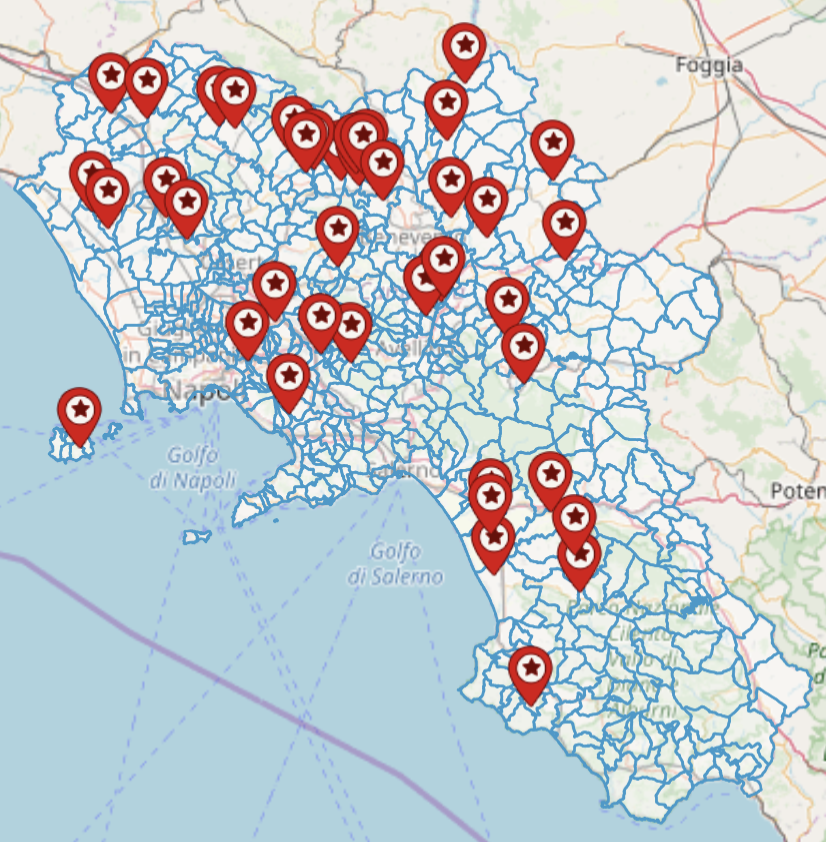
\includegraphics[scale=.8]{figures/rarLocations}
    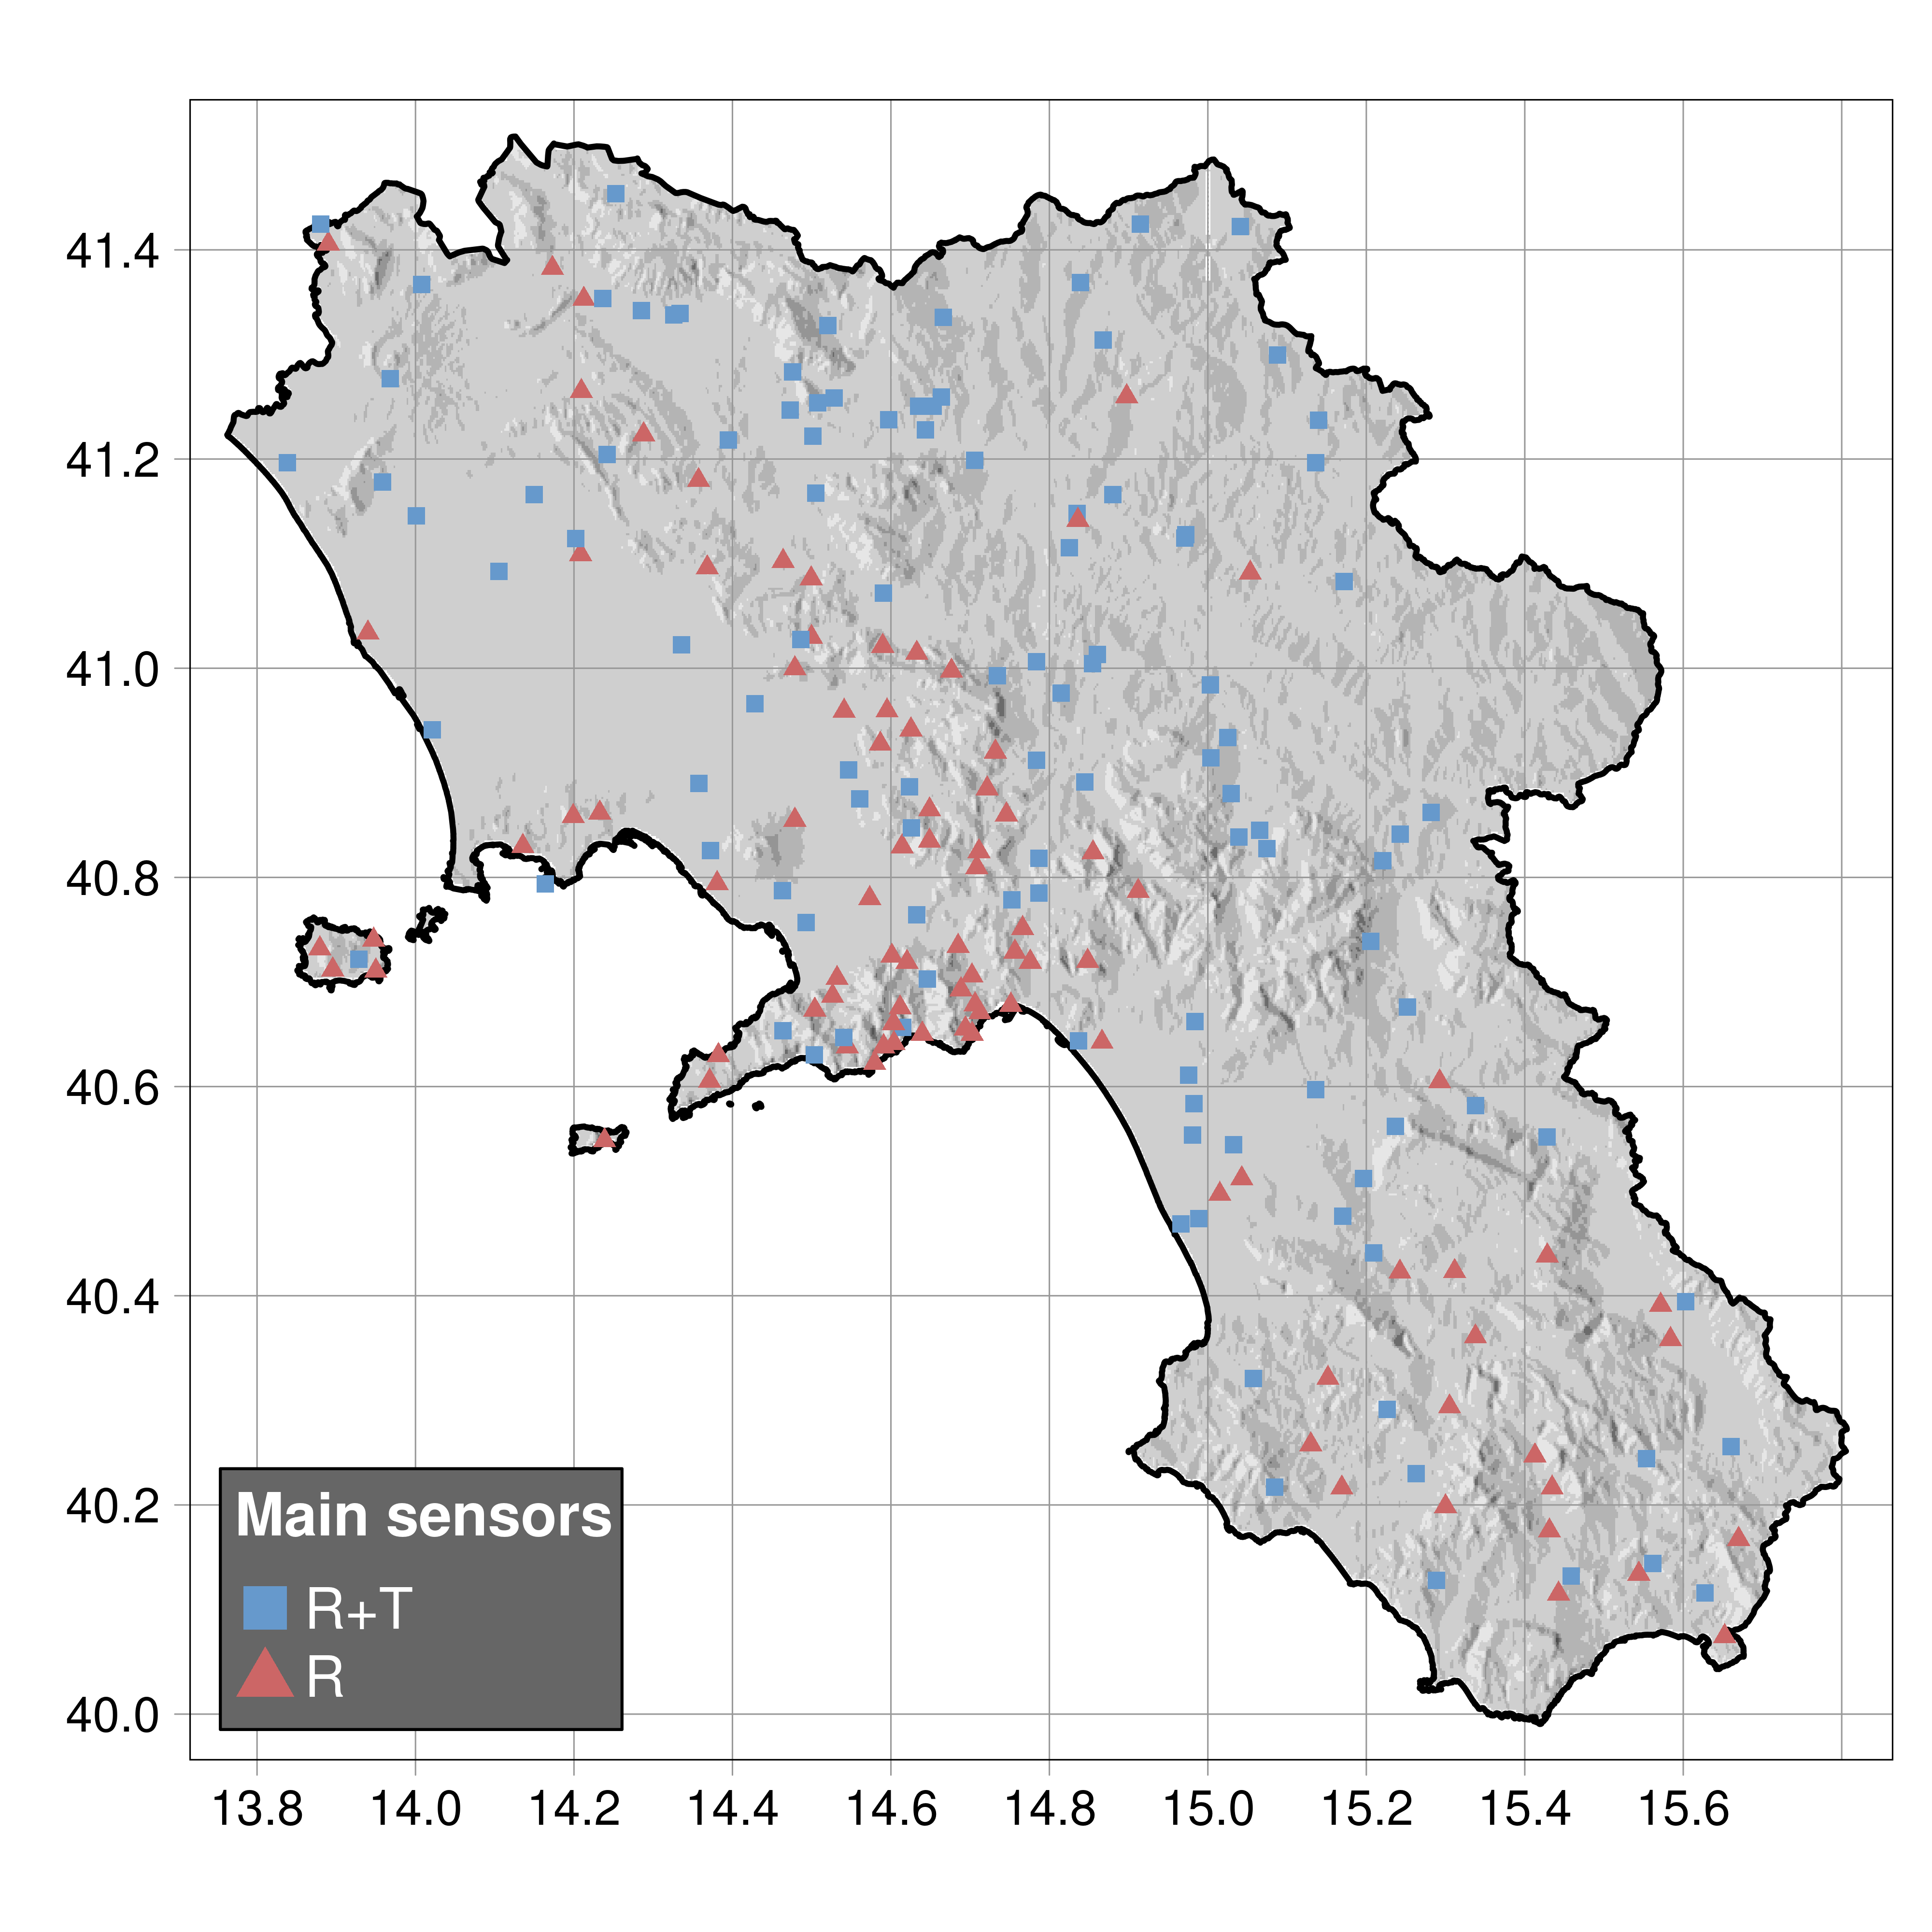
\includegraphics[scale=0.6]{figures/map_stations.png}
	\caption{ Geolocation of the stations included in the agrometeorological database of Campania Region, \DIFdelbeginFL \DIFdelFL{including }\DIFdelendFL %DIF >  including both agrometeorological and hydrometeorological networks.
    \DIFaddbeginFL \DIFaddFL{encompassing }\DIFaddendFL both agrometeorological and hydrometeorological networks. \DIFdelbeginFL \DIFdelFL{The }\DIFdelendFL \DIFaddbeginFL \DIFaddFL{These }\DIFaddendFL stations \DIFdelbeginFL \DIFdelFL{available are grouped by symbol type }\DIFdelendFL \DIFaddbeginFL \DIFaddFL{play a crucial role in monitoring regional climate conditions, supporting agricultural management, }\DIFaddendFL and \DIFdelbeginFL \DIFdelFL{color according to the main sensors available}\DIFdelendFL \DIFaddbeginFL \DIFaddFL{hydrological assessments}\DIFaddendFL .
    \DIFdelbeginFL \DIFdelFL{There are stations having both rain and air temperature sensors or stations having either a rain or an air temperature sensor.}\DIFdelendFL %DIF >  The stations available are grouped by symbol type and color according to the main sensors available. There are stations having both rain and air temperature sensors or stations having either a rain or an air temperature sensor.
    }
	\label{fig:rarLocations}
\end{figure}

The monitoring network is in charge of the Agrometereological Regional Centre (CAR, \emph{Centro Agrometereologico Regionale}) under the Department for Agriculture of the Campania Region. The CAR is also in charge of producing pest risk bulletins for the agricultural farms of the Region.

\subsubsection{Hydrogeological risk monitoring network\label{DPCNetwork}}
The hydrogeological risk monitoring network comprises \DIFdelbegin \DIFdel{, at the time of this writing, }\DIFdelend %DIF > , at the time of this writing, 
172 stations\DIFdelbegin \DIFdel{within the administrative boundaries of the Campania Region. }\DIFdelend \DIFaddbegin \DIFadd{. %DIF >  within the administrative boundaries of the Campania Region.
}\DIFaddend Despite the significant number of monitoring \DIFdelbegin \DIFdel{points}\DIFdelend \DIFaddbegin \DIFadd{locations}\DIFaddend , this network is not especially suitable for agroclimatic-oriented weather monitoring out of the box, since its main purpose is different.
\DIFdelbegin \DIFdel{This is reflected in both the geographical distribution of the stations, more focused on areas at high hydrogeological risk rather than cultivated lands, and in their instrumentation.
In fact, apart from thermometers and pluviometers, stations of this network are variously equipped with a range of sensors, most of which are irrelevant to the agrometereological monitoring.
This means that only }\DIFdelend %DIF > This is reflected in both the geographical distribution of the stations, more focused on areas at high hydrogeological risk rather than cultivated lands, and in their instrumentation.
%DIF > In fact, apart from thermometers and pluviometers, stations of this network are variously equipped with a range of sensors, most of which are irrelevant to the agrometereological monitoring.
\DIFaddbegin \DIFadd{However, a substantial amount of }\DIFaddend air temperature and rainfall data \DIFdelbegin \DIFdel{are available }\DIFdelend from this network \DIFaddbegin \DIFadd{has been successfully integrated with the CAR network within AgriMetSupport}\DIFaddend .
\DIFdelbegin %DIFDELCMD < 

%DIFDELCMD < %%%
\DIFdel{For these reasons, a filtering has been performed prior to the integration in AgriMetSupport.
Only stations deployed at locations deemed of interest, and with suitable equipment, for agrometereological monitoring, have been included in the infrastructure.
Nevertheless, the integration of this network made possible by AgriMetSupportallow to dramatically improve the coverage at least for the two available climatic parameters.
}%DIFDELCMD < 

%DIFDELCMD < %%%
\DIFdelend %DIF > For these reasons, a filtering has been performed prior to the integration in AgriMetSupport.
%DIF > Only stations deployed at locations deemed of interest, and with suitable equipment, for agrometereological monitoring, have been included in the infrastructure.
%DIF > Nevertheless, the integration of this network made possible by AgriMetSupport allow to dramatically improve the coverage at least for the two available climatic parameters.
The monitoring network is managed by the Civil Protection Agency of the Campania Region (DPC, Dipartimento Protezione Civile)\DIFdelbegin \DIFdel{, which contributes its data through a partnership with the CAR. }\DIFdelend \DIFaddbegin \DIFadd{. %DIF > , which contributes its data through a partnership with the CAR.
}\DIFaddend 

\subsection{Retrieve and decode bulletin data}
\DIFaddbegin \statusblock{}{wip}{REVIEW THIS SECTION HAVING IN MIND THE NEW FIGURES, SPECIALLY \cref{Box01:WeatherProg_Operations}.}

\DIFaddend On hourly basis, CAR and DPC send each a bulletin containing the 10-minute measurements of the last 24 hours.
Each entry of the bulletin represents a point in time and includes the values of all the variables measured by any station.
The two bulletins are sent via sFTP to a server located on the premises of the CRISP\footnote{CRISP is an Interdepartmental Research Centre of the University of Naples Federico II focusing on the \textit{Earth Critical Zone}.}.

%As said earlier, data is sent from CAR on an hourly basis, containing all the measurements of the previous 24 hours.
To handle the hourly dispatch and provide data to the end users as soon as they are available, the system is configured to automatically have a run of WeatherProg every hour on both CAR and DPC networks, according to the schedule in \cref{Fig:weatherprog:calls}.
This hourly run is responsible for updating the database with the raw data related to the last hour.
Late updates of the incoming data are dealt with by a periodic run of a reanalysis pipeline, on both daily and monthly basis.
%This daily run works on the whole 24-hour incoming table, check which time ranges are missing within the database and fills them.

% The first part of the validation study was performed in the gpu-pedology VM using matlab-vnc instance.
%  - open the VNC client pointing to gpu-pedology
%  - http://192.168.20.10:6080/vnc.html?password=matlab&autoconnect=true&resize=remote
%  - git: search for "perturbation" in tree
%  - folder: run#paper
%  The second part of the validation study was performed on Pedometrics VM (e.g. use of "versions" in .mat files)
%  - folder on Pedometrics VM: /home/giuliano/work/Projects/URCOFI/run#paper/TABLES/
%DIF > \subsection{Validation of quality control and gap-filling procedures} \label{sec:QcheckValidation}
\subsection{\DIFdelbegin \DIFdel{Validation of }\DIFdelend \DIFaddbegin \DIFadd{Procedure for validating }\DIFaddend quality control and gap-filling \DIFdelbegin \DIFdel{procedures}\DIFdelend \DIFaddbegin \DIFadd{methods}\DIFaddend } \label{sec:QcheckValidation}
\DIFdelbegin \DIFdel{AgriMetSupport }\DIFdelend \DIFaddbegin \DIFadd{Agri\-Met\-Support }\DIFaddend enables the management of agrometeorological data using fully automated or semi-automated procedures. % which belongs above all to the WeatherProg engine.
\DIFdelbegin \DIFdel{A user of AgriMetSupport should always be aware of the level of confidence and reliability associated with the use of each internal component, with particular emphasis here on WeatherProg and its constituent modules as they were shown in \mbox{%DIFAUXCMD
\cref{sec:weatherprog}}\hskip0pt%DIFAUXCMD
. 
}\DIFdelend \DIFaddbegin \statusblock{}{wip}{MODIFY ACCORDING TO Q6R3 POINT (2). A user of Agri\-Met\-Support should always be aware of the level of confidence and reliability associated with the use of each internal component, with particular emphasis here on WeatherProg. % and its constituent modules as they were shown in \cref{sec:weatherprog}.
}
\DIFaddend To achieve this objective, WeatherProg was equipped with a smart deviation from its standard run.
In other words, it was equipped with a switch capable to introduce random noise in the raw data and then measure its own performance in fixing them. % known anomalous data.
Reproducible random noise is generated on-the-fly in the run and \DIFdelbegin \DIFdel{it }\DIFdelend is never stored in the database.

A validation study was carried out for the scope of this article on 10-minute air temperature data, in the year 2021, for both RAR and DPC networks, in both quality control and infill modules.
The deviation or switch was introduced in the 10-minutes pipeline tackling the daily run dedicated to the creation of no-gap and certified data, as depicted in \cref{Fig:weatherprog:calls} .%\note{(MODIFY THE FIGURE TO ADD THE DEVIATION/SWITCH GRAPHICALLY))}.
The insert of noise simulates what could actually happen if receiving true anomalous data but forcing perturbed signals to overstress the WeatherProg modules.
\DIFdelbegin \DIFdel{If the perturbation switch is active, noisy data are }\DIFdelend \DIFaddbegin \DIFadd{To perform the validation study, the perturbation switch was activated and noisy data were }\DIFaddend created according to \DIFdelbegin \DIFdel{different levels of absolute amplitude }\DIFdelend \DIFaddbegin \DIFadd{two key parameters:
}\begin{itemize}
    \item \DIFadd{Amplitude }\DIFaddend ($A$)\DIFdelbegin \DIFdel{and quota ($Q$), where amplitude is }\DIFdelend \DIFaddbegin \DIFadd{, }\DIFaddend a magnitude exaggeration factor \DIFdelbegin \DIFdel{applied to air temperature }\DIFdelend \DIFaddbegin \DIFadd{used to scale random numbers generated in the range from zero to one into air temperature values }\DIFaddend (in this validation study\DIFdelbegin \DIFdel{$A$ is set to its maximum, that is }\DIFdelend , \DIFdelbegin \DIFdel{$A=10$)while quota accounts for the relative amount }\DIFdelend \DIFaddbegin \DIFadd{$A=10$). For instance, if the random number generated is equal to 0.87 and the air temperature measurement is \mbox{%DIFAUXCMD
\SI{22.4}{\degreeCelsius} }\hskip0pt%DIFAUXCMD
then the perturbed value is $0.87\times10 + 22.4 = \SI{31.1}{\degreeCelsius}$.
    }\item \DIFadd{Quota ($Q$), representing the proportion }\DIFaddend of raw measurements into which noise is inserted ($Q=30\%$ in this validation study).
\DIFaddbegin \end{itemize}
\DIFaddend The following procedure was repeated for each of the 30
% remove 2 days with huge missings + change the figure
randomly selected days within the year 2021, where each day has \DIFdelbegin \DIFdel{$N_{rec}=12816$ }\DIFdelend \DIFaddbegin \DIFadd{potentially $N_{rec}=12,816$ }\DIFaddend records (i.e., 144 \DIFdelbegin \DIFdel{10-minutes }\DIFdelend \DIFaddbegin \DIFadd{10-minute }\DIFaddend records $\times$ 89 stations measuring air temperature):

\begin{enumerate}
    \item get the number of $N$ records to which add noise, \DIFdelbegin \DIFdel{$N = int( N_{rec} * Q ) = int(12816 \times 30 / 100) = 3845$}\DIFdelend \DIFaddbegin \DIFadd{$N = int( N_{rec} * Q ) = int(12,816 \times 30 / 100) = 3,845$}\DIFaddend ;
    \item get the vector $P_{idx}$ of $N$ random row indexes out of $N_{rec}$ daily raw records stored in the data frame $RawData[\,N_{rec}\,,\,Air \; Temperature\,]$;
    \item get the sign vector $S_{(\pm)}$ of length $N$ made by a random sequence of $+$ and $-$ signs (i.e. a sequence of $+1$ and $-1$);
    \item generate a vector $R_{abs}$ of absolute random numbers of length $N$ from a uniform [0,1] distribution;
    \item put $N$ noisy values in the data frame $RawData$ at $P_{idx}$ random row indexes as follows:
    %$$
    \begin{multline}
    RawData[\,P_{idx}\,,\,Air \; Temperature\,] = \\
    RawData[\,P_{idx}\,,\,Air \; Temperature\,] + S_{(\pm)} \times R_{abs} \times A      
    \end{multline}
    %$$
\end{enumerate}

\DIFaddbegin \DIFadd{Each time a random generation mechanism is used (steps 2,3, and 4), the seed is set to a predefined value to ensure experiment's repeatability.
}

\begin{table}[h]
    \begin{tiny}
    \centering
    %DIF > \renewcommand{\arraystretch}{1.2} % Adjust row height for readability
    \begin{tabular}{lcccccccccc}  %DIF >  Reduced to match actual column count
        \toprule
        \textbf{\DIFaddFL{Variable}} & \textbf{\DIFaddFL{Count}} & \textbf{\DIFaddFL{Mean}} & \textbf{\DIFaddFL{SD}} & \textbf{\DIFaddFL{Median}} & \textbf{\DIFaddFL{Min}} & \textbf{\DIFaddFL{Max}} & \textbf{\DIFaddFL{Mode}} & \textbf{\DIFaddFL{Skew.}} & \textbf{\DIFaddFL{Kurt.}} & \textbf{\DIFaddFL{IQR}} \\
        \midrule
        \multicolumn{11}{l}{\textbf{\DIFaddFL{January 1, 2021 (Julian Day 1)}}} \\
        \DIFaddFL{Raw unperturbed  }& \DIFaddFL{8860  }& \DIFaddFL{6.50  }& \DIFaddFL{2.92  }& \DIFaddFL{6.5   }& \DIFaddFL{-3.4  }& \DIFaddFL{14.6  }& \DIFaddFL{5.5   }& \DIFaddFL{-0.10  }& \DIFaddFL{-0.36  }& \DIFaddFL{4.3  }\\
        \DIFaddFL{Raw before       }& \DIFaddFL{3795  }& \DIFaddFL{6.54  }& \DIFaddFL{2.93  }& \DIFaddFL{6.6   }& \DIFaddFL{-3.3  }& \DIFaddFL{14.7  }& \DIFaddFL{5.5   }& \DIFaddFL{-0.10  }& \DIFaddFL{-0.38  }& \DIFaddFL{4.4  }\\
        \DIFaddFL{Perturbed        }& \DIFaddFL{3795  }& \DIFaddFL{6.56  }& \DIFaddFL{6.53  }& \DIFaddFL{6.61  }& \DIFaddFL{-12.6 }& \DIFaddFL{22.4  }& \DIFaddFL{-0.97 }& \DIFaddFL{-0.05  }& \DIFaddFL{-0.77  }& \DIFaddFL{10.4 }\\
        \midrule
        \multicolumn{11}{l}{\textbf{\DIFaddFL{July 19, 2021 (Julian Day 200)}}} \\
        \DIFaddFL{Raw unperturbed  }& \DIFaddFL{8932  }& \DIFaddFL{21.6  }& \DIFaddFL{3.48  }& \DIFaddFL{21.2  }& \DIFaddFL{12.6  }& \DIFaddFL{32.7  }& \DIFaddFL{18.7  }& \DIFaddFL{0.39   }& \DIFaddFL{-0.49  }& \DIFaddFL{5.2  }\\
        \DIFaddFL{Raw before       }& \DIFaddFL{3828  }& \DIFaddFL{21.5  }& \DIFaddFL{3.48  }& \DIFaddFL{21.0  }& \DIFaddFL{12.5  }& \DIFaddFL{32.8  }& \DIFaddFL{17.7  }& \DIFaddFL{0.41   }& \DIFaddFL{-0.48  }& \DIFaddFL{5.2  }\\
        \DIFaddFL{Perturbed        }& \DIFaddFL{3828  }& \DIFaddFL{21.3  }& \DIFaddFL{6.85  }& \DIFaddFL{21.3  }& \DIFaddFL{3.95  }& \DIFaddFL{40.1  }& \DIFaddFL{17.4  }& \DIFaddFL{0.07   }& \DIFaddFL{-0.72  }& \DIFaddFL{10.4 }\\
        \bottomrule
    \end{tabular}
    \caption{\DIFaddFL{Summary statistics for air temperature on January 1, 2021 and July 19, 2021 accoroding to perturbation.}}
    \label{tab:stats_perturbation}    
    \end{tiny}
    %DIF >  12655 records on day 001
    %DIF >  12760 records on day 200
\end{table}

\statusblock{}{wip}{[Q3R1] Explicitly describe the **statistical properties** of the noise introduced (e.g., distribution, magnitude, frequency).}

%DIF >  Skewness:
%DIF >    It is a measure of symmetry, or more precisely, the lack of symmetry. A distribution, or data set, is symmetric if it looks the same to the left and right of the center point.
%DIF >  Kurtosis:
%DIF >    It is a measure of whether the data are heavy-tailed or light-tailed relative to a normal distribution.
\DIFadd{\mbox{%DIFAUXCMD
\cref{tab:stats_perturbation} }\hskip0pt%DIFAUXCMD
provides main statistics on air temperature data in relationship to the perturbation procedure, with two distinct days shown as examples.
To analyze the effect of perturbation on the statistical properties of air temperature, it is necessary to distinguish between raw unperturbed data (unchanged after perturbation), raw data before perturbation (original values prior to modification), and perturbed data (raw data that has been altered by the perturbation process).
%DIF > Even though comparing two days may not be entirely relevant, January 1, 2021 (winter) exhibits a lower mean temperature (\SI{6.5}{\degreeCelsius}) and is slightly skewed to the left, whereas July 19, 2021 (summer) has a significantly higher mean temperature (\SI{21.6}{\degreeCelsius}) and is strongly skewed to the right.
The perturbation mechanism exhibits a similar effect across seasons, despite differences in absolute temperature values. On both January 1, 2021 (winter) and July 19, 2021 (summer), perturbation increases the variability of air temperature measurements, as reflected in the higher standard deviation and interquartile range. This suggests that the perturbation process operates independently of seasonal temperature variations, preserving its statistical impact regardless of the underlying temperature distribution.
There is no difference (all statistics are the same) between the unperturbed raw data and the raw data selected for perturbation, confirming the robustness of the random selection mechanism in determining which data points are then perturbed.
%DIF > The interquartile range (IQR) and the standard deviation (SD) are larger in July, suggesting more variability in temperature during summer.
}\begin{figure}[th]
	\centering
    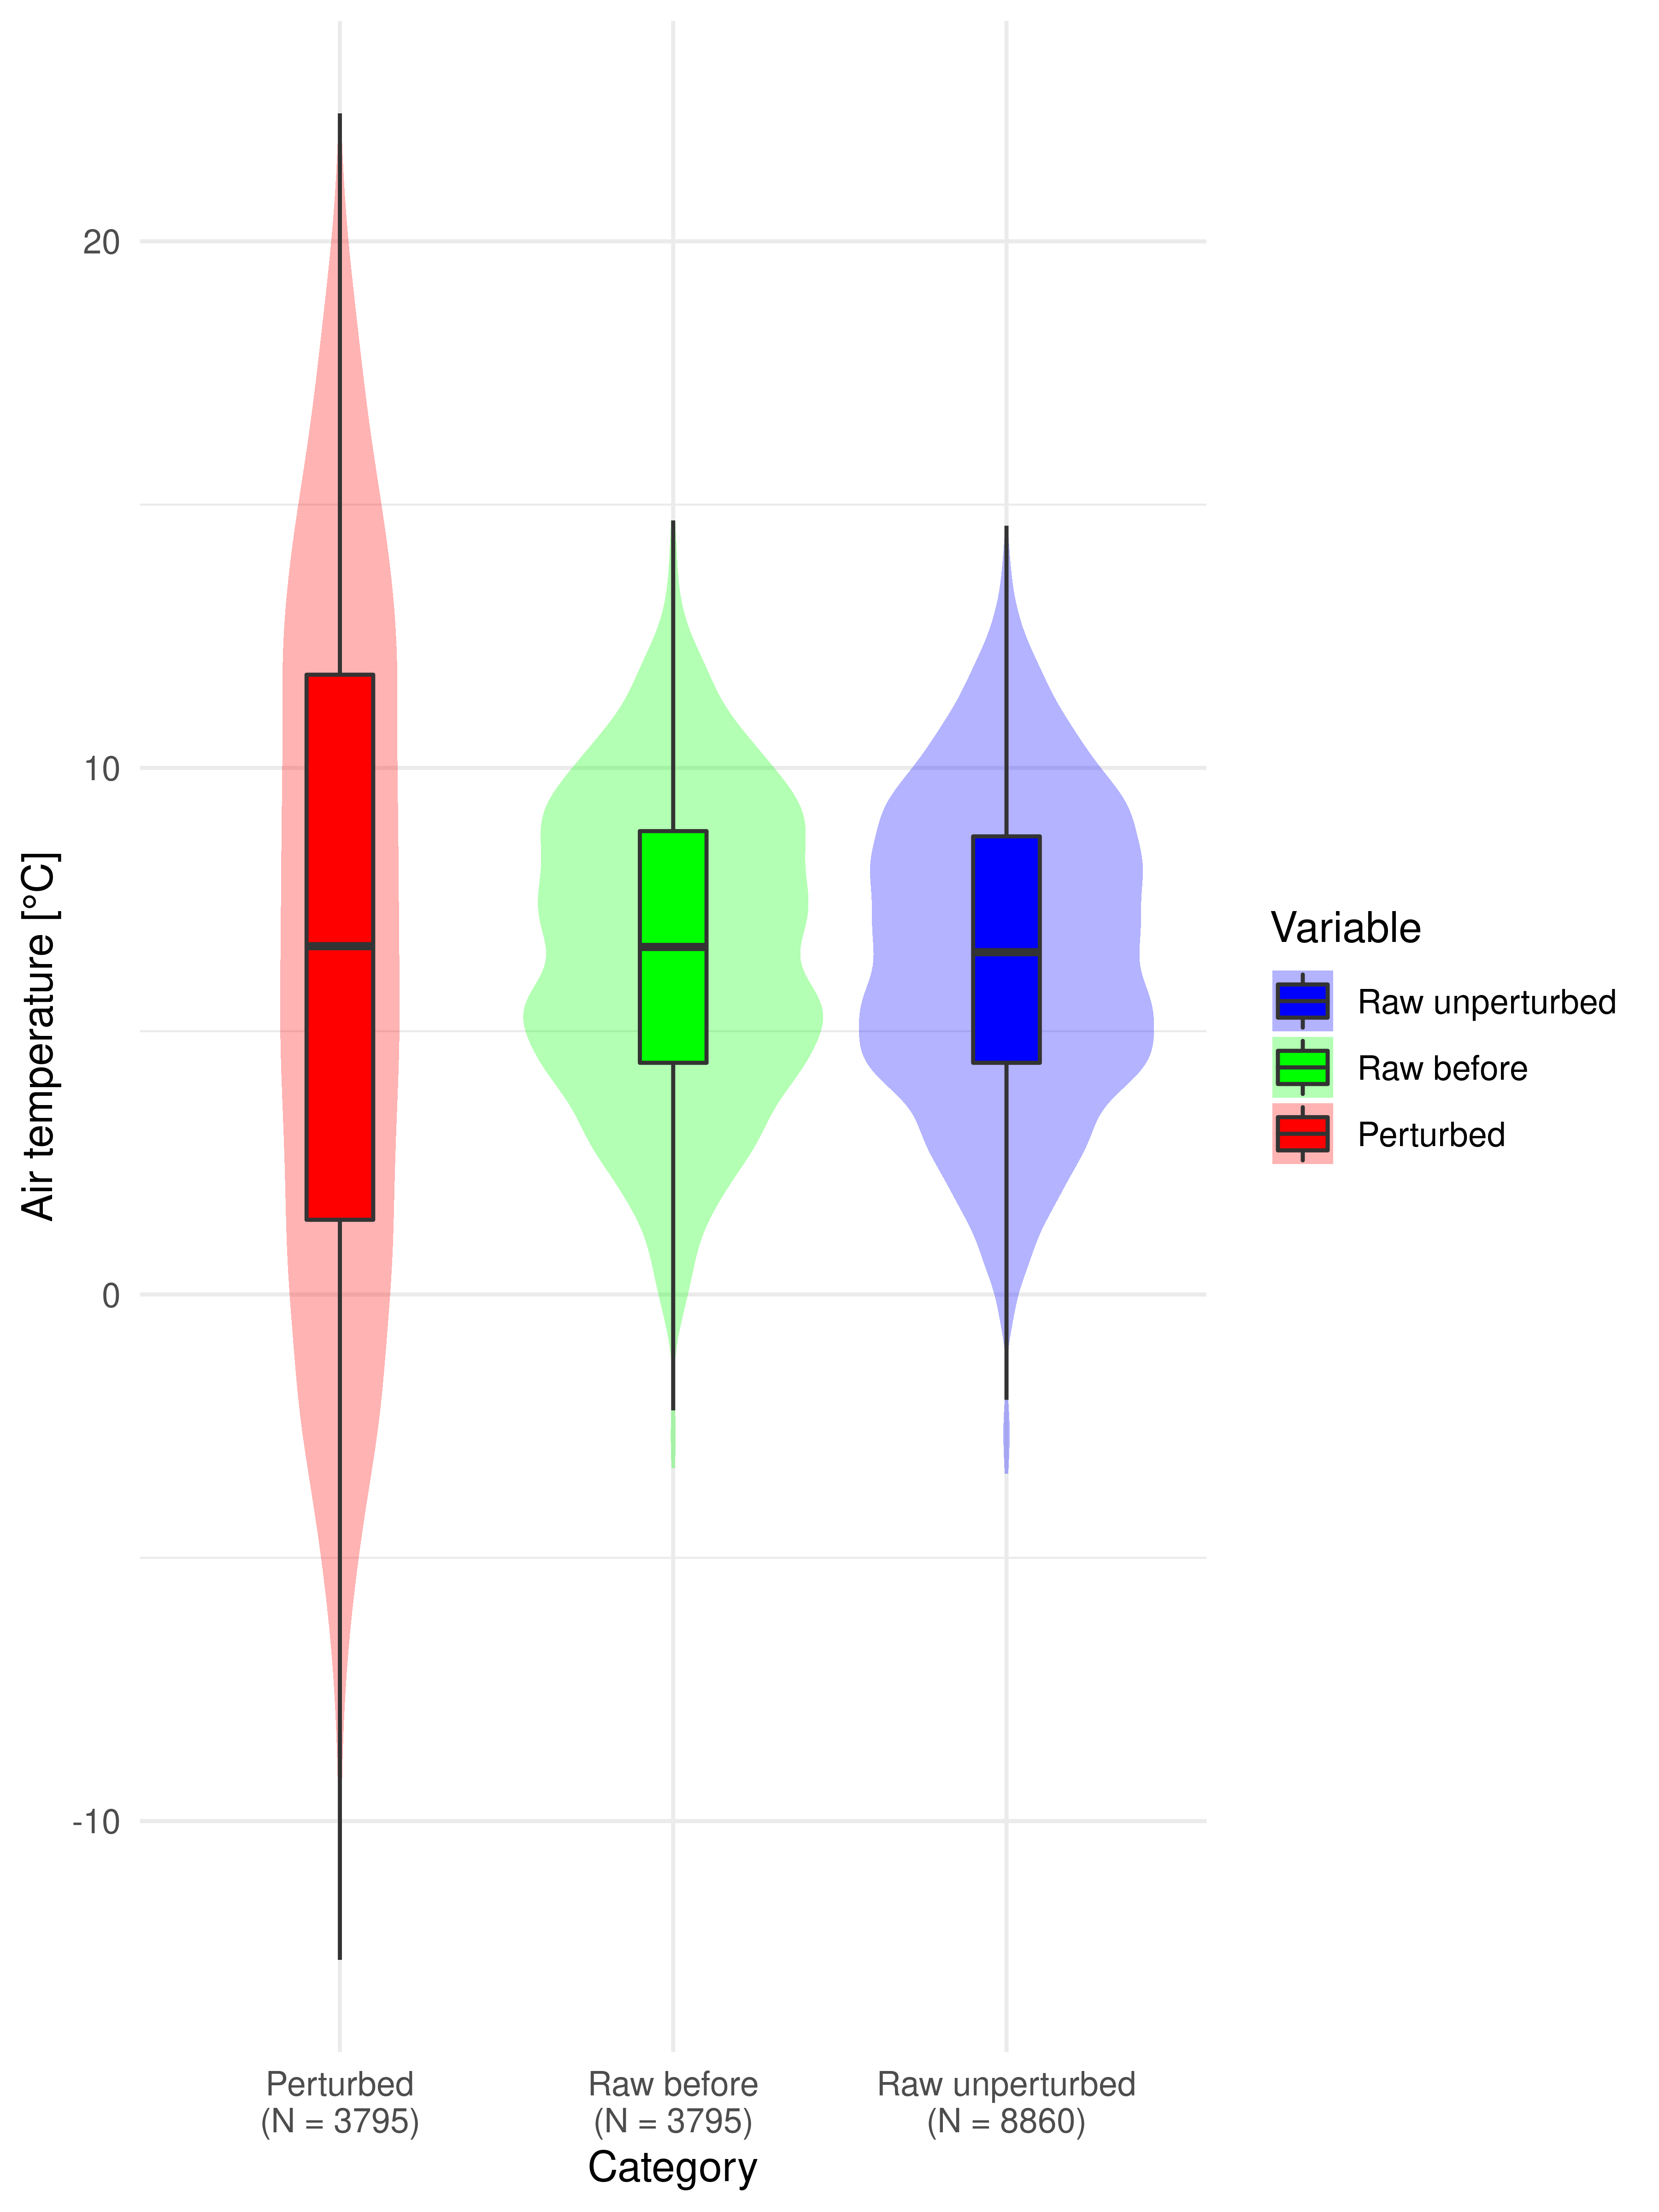
\includegraphics[scale=0.4]{figures/boxplot_perturbation.png}
	\caption{ \DIFaddFL{Frequency distribution for January 1, 2001. 
              The raw data selected for perturbation has the same distribution as the unperturbed raw data but differs from the perturbed data, as also shown in \mbox{%DIFAUXCMD
\cref{tab:stats_perturbation}}\hskip0pt%DIFAUXCMD
. }}
	\label{fig:perturbation_freqDistr}
\end{figure}
\DIFadd{Perturbed data shows the same mean and median of raw data (both unperturbed raw data and the raw data selected for perturbation), while it consistently shows an increase in standard deviation and interquartile range (\mbox{%DIFAUXCMD
\cref{fig:perturbation_freqDistr}}\hskip0pt%DIFAUXCMD
), confirming that the perturbation introduces additional variability, as expected to run the validation procedure.
The mode shift in the perturbed dataset from \mbox{%DIFAUXCMD
\SI{5.5}{\degreeCelsius} }\hskip0pt%DIFAUXCMD
to \mbox{%DIFAUXCMD
\SI{-0.97}{\degreeCelsius} }\hskip0pt%DIFAUXCMD
in January, demonstrates its inconsistency to make comparisons on a continuous variable.
Minimum and maximum values for perturbed data differ significantly from raw data, consistently across both winter and summer days, with the range extending from \mbox{%DIFAUXCMD
\SI{-12.6}{\degreeCelsius} }\hskip0pt%DIFAUXCMD
in winter to \mbox{%DIFAUXCMD
\SI{40.1}{\degreeCelsius} }\hskip0pt%DIFAUXCMD
in summer. These extreme values, along with all intermediate ones, are what the validation procedure considers when assessing WeatherProg's ability to detect and fill anomalies.
%DIF > The kurtosis values are negative, with perturbed data showing less negative values, indicating a more uniform distribution with fewer extreme outliers than a normal distribution.
}

\DIFadd{The correlation between raw and perturbed air temperature data in relation to air humidity, grouped by station,  shows an overall percentage change in correlation ranging from 2.99\% to 22.03\%, with a median of 6.94\% and a mean of 7.46\%.  
This variation suggests that the perturbation mechanism introduces statistically controlled changes while preserving a strong relationship with environmental variables such as air humidity.  
These results confirm that the perturbation process does not disrupt the intrinsic correlation structure between air temperature and atmospheric humidity across different locations, ensuring that the system validation approach remains representative of real-world agricultural conditions.
}

\DIFadd{These perturbation statistics are presented here to validate and demonstrate the robustness of the validation methodology itself, rather than as main findings, which are presented separately in \mbox{%DIFAUXCMD
\cref{Results-Discussion}}\hskip0pt%DIFAUXCMD
.
}

\statusblock{}{wip}{any reference to infill is not yet written here. Currently, I decide that no reference to infill must be provided here since it is shown in results. Here we only have the part related to the building of the validation procedure.}


\DIFaddend %according to the different modules (qcheck, infill, tscale aggregation) including a manual implementation of a geostatistical analysis (variogram + kriging with err.var). I evaluate the propagation of uncertainty in other calculations using agrometeo data, such as bioclimatic indices or simulation models, such as plasmorossi using hourly data.
% Finally, I collect all the errors made in comparison with the original non-perturbed data, such as:
% [on 10-min data]
%   > N of data not passig qcheck but good; (false negative, FN)
%   > N of data passing qcheck but bad;     (false positive, FP)
%   > rmse on meas vs pert data FN & FP;    (rmse on FN & FP)
%   > rmse on infilled vs measured data;    (skip)
% [on h1 data, after h1 qcheck + infill]
%   > develop a procedure to validate WeatherProg processing with
%     plasmorossi.
% [on h24 data, after h24 qcheck + infill]
%   > N of data not passig qcheck but good;
%   > N of data passing qcheck but bad;
%   > rmse on infilled vs measured data;
%   > GDD;
%   > kriging variance error.
% [on h24 data, aggregated without 10-min qcheck + infill]
%   > same as previous block
% Finally, I have to compare data at h1 / h24 before / after data curation: it means that I should calculate the statitistcs or run models also on data without qcheck + infill to compare with the situation in which I use weatherprog for data curation (qcheck + infill) and get a quantitative mesurement of the usefulness of WeatherProg.

%We can think to a WeatherProg module as a black box to which agrometeorological data is passed as input and additional information (metadata) is attached to the original raw data, such as flags concerning the quality check procedure or infilled values which are predicted values substituting the raw ones because of their poor reliability.
%This knowledge was used to enhance results coming from WeatherProg with particular reference to the quality check module and the gaps infilling module.

\DIFaddbegin \subsection{\DIFadd{AgriMetSupport quality assessment}}
\statusblock{}{wip}{The quality of the AgriMetSupport system is evaluated based on several performance criteria, excluding assessments related to the system as a whole, such as decision support, user interaction efficiency, data dissemination effectiveness, and integration with external services.
Instead, the evaluation presented in this paper focuses on WeatherProg performance, which may vary depending on the configuration of a specific AgriMetSupport instance and, consequently, on the scheduling of pipelines.
In general, the criteria account for the system ability to produce continuous hourly and daily time series without gaps, as well as to generate hourly and daily spatial maps.
Specifically, an internal assessment is performed to monitor the system performance, to score it and then trigger alerts based on:
\begin{itemize}
    \item The amount of data delivered (e.g., missing or incomplete records compared to expectations). Some thresholds are considered internally to avoid inconsistencies in the data, such as too many gaps (i.e. 30\%) for a particular station or a specific time element. An alert is generated and shared with data providers to acknowledge possible issues in the whole pipeline including the sensor, the station, the communication channel, the data provider database and relative management software, the data delivery mechanism, the AgriMetSupport API, the WeatherProg engine, and finally the internal point and raster databases.
    % I make examples to reply to possible comments by reviewers: for instance  why there is an issue about WeatherProg engine relaated to the amount of data delivered? Because issues can arise at any point in the pipeline in case data with gaps are delivered.
    \item The proportion of data that fails the quality control process, relative to the expected performance of approximately 90\%, which is assessed through the perturbation mechanism introduced during the validation procedure. An alert is generated to ensure that data streams and processing are functioning correctly.
    \item A cross-validated linear regression method is applied to each reconstructed datum, providing a direct measure of the system’s ability to generate real-time gap-filled data with reliable accuracy. An alert is generated if the RMSE exceeds a configurable threshold (e.g. \SI{1.5}{\degreeCelsius} for air temperature) over a significant portion of reconstructed data.
    \item The persistence of gaps after time series aggregation, quality control, and gap-filling, as these can hinder the ability to feed downstream applications, such as dashboards and services. No more than one gap per day and station is allowed and an alert is generated to signal potential issues and ensure timely intervention.
\end{itemize}
%The perturbation analysis, available through the validation procedure, quantifies the proportion of erroneous data, offering a means to track the accuracy of anomaly detection over time.
}

\DIFaddend % The second part of the validation study was performed on Pedometrics VM (e.g. use of "versions" in .mat files)
%  - folder on Pedometrics VM: /home/giuliano/work/Projects/URCOFI/run#paper/TABLES/
% Use the previous folder to analyse results.
\section{Results and Discussion} \DIFdelbegin \DIFdel{AgriMetSupport }\DIFdelend \DIFaddbegin \label{Results-Discussion}

\subsection{\DIFadd{AgriMetSupport CPS}}
\DIFadd{Agri\-Met\-Support }\DIFaddend exemplifies a model \DIFdelbegin \DIFdel{GCI }\DIFdelend \DIFaddbegin \DIFadd{geospatial CPS }\statusblock{}{wip}{(I decided to remove GCI from the whole paper and use CPS instead)}  \DIFaddend that can be seamlessly customised to manage sensor networks across several territories.
Its design underscores pronounced multi-level granularity,
particularly evident in the flexibility afforded by its containerized deployment architecture. 
This granularity enables the distribution of its stack across the internet, for instance, allowing the data tier and the presentation tier to interoperate from distinct geographical locations. 
Moreover, the capacity to instantiate separate Docker containers for production pipelines (\cref{Fig:weatherprog:calls}) and testing or debugging purposes facilitates a robust development lifecycle.
Distinct databases for development and production -- associated to two different WeatherProg instances -- further enhance this segregation, ensuring that data integrity and application stability are maintained.

At a physical level, \DIFdelbegin \DIFdel{AgriMetSupport}\DIFdelend \DIFaddbegin \DIFadd{Agri\-Met\-Support}\DIFaddend 's granularity allows for the integration and management of disparate monitoring networks within a unified infrastructure.
This capability was demonstrated in the Campania Region case study, which showed the integration of CAR and DCP networks.
Furthermore, the system's architecture supports the incorporation of smart and low-cost stations, satisfying the requirements of precision agriculture and advanced Internet of Things (IoT) applications. %, albeit these applications were not explored in the case study for brevity.

\DIFdelbegin %DIFDELCMD < \begin{figure}
%DIFDELCMD < 	\centering
%DIFDELCMD < 	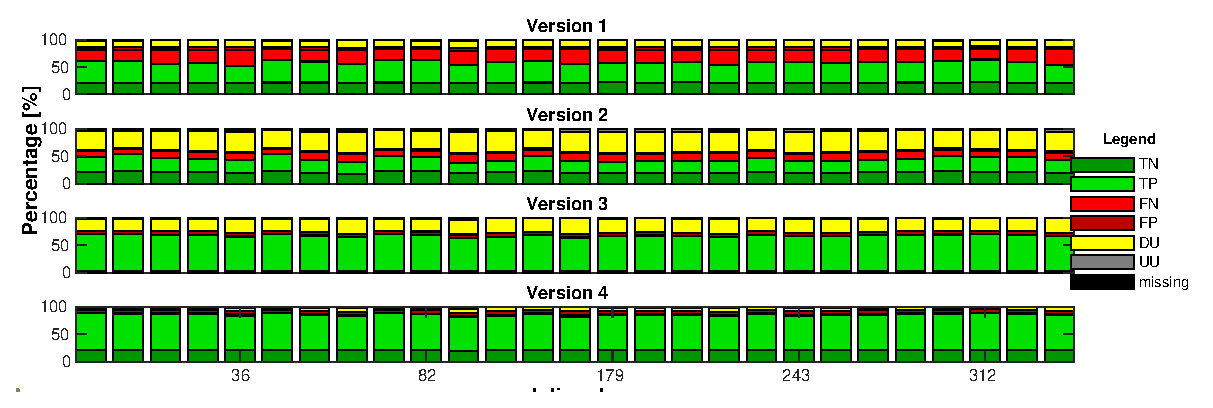
\includegraphics[scale=.30]{figures/Fig_qck_versions_v2.tif}
%DIFDELCMD < 	%%%
%DIFDELCMD < \caption{%
{%DIFAUXCMD
\DIFdelFL{Evolution performance of the air temperature quality control procedure on randomly selected Julian days in year 2022.
    Details about versions: version 1 uses a preliminary version of range, persistence and continuity control types; version 2 adds spatial control type to version 1; version 3 introduces enhancements to the continuity and spatial control types while reducing the amount of dubious outcomes; version 4 implements a smarter quality control logic, as reported in \mbox{%DIFAUXCMD
\cref{tab:qcheck_m10_airT}}\hskip0pt%DIFAUXCMD
.
    Details about legend. TN: true negative; TP: true positive; FN: false negative; FP: false positive; DU: dubious; UU: undecided or unprocessed. }}
	%DIFAUXCMD
%DIFDELCMD < \label{fig:perturbationCharts}
%DIFDELCMD < \end{figure}
%DIFDELCMD < 

%DIFDELCMD < %%%
\DIFdelend \DIFaddbegin \subsection{\DIFadd{WeatherProg engine}}
\DIFaddend %The schedule of pipelines execution depicted in \cref{Fig:weatherprog:calls} is a clear evidence of a further level of granularity available within WeatherProg, which is the backbone engine of the whole cyber-physical system.
WeatherProg, serving as the backbone engine of \DIFdelbegin \DIFdel{AgriMetSupport}\DIFdelend \DIFaddbegin \DIFadd{Agri\-Met\-Support}\DIFaddend , facilitates a detailed and user-friendly management of standard, reanalysis, or recursive pipelines, as clearly highlighted in the \DIFdelbegin \DIFdel{schedule }\DIFdelend \DIFaddbegin \DIFadd{job scheduling }\DIFaddend shown in \cref{Fig:weatherprog:calls}.
This includes the activation of specific modules such as data decoding, quality control, and data infilling, tailored to particular monitoring networks, agrometeorological variables, and spatial and temporal scales.

The validation study performed on WeatherProg's quality control and data infilling modules illustrates the system's adeptness at processing and refining meteorological data (\cref{fig:perturbationCharts}).
Using artificially perturbed data -- as explained in the noisy data generation given in \cref{sec:QcheckValidation} -- in place of raw measurements from Regional bulletins allowed for a direct comparison of WeatherProg's capabilities in anomaly detection and data correction against the raw, original, and unaltered observations.

\DIFaddbegin \begin{figure}
	\centering
	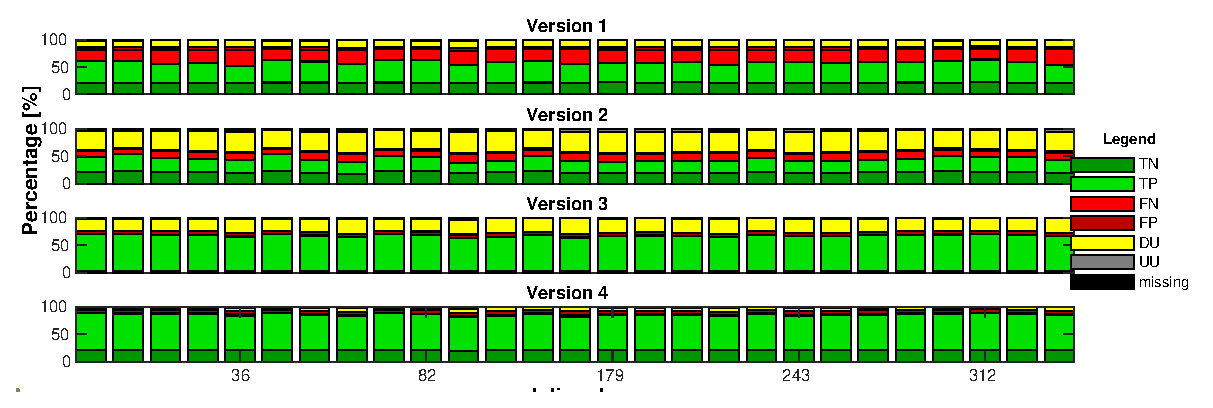
\includegraphics[scale=.30]{figures/Fig_qck_versions_v2.tif}
	\caption{ \DIFaddFL{Evolution performance of the air temperature quality control procedure on randomly selected Julian days in year 2022.
    Details about versions: version 1 uses a preliminary version of range, persistence and continuity control types; version 2 adds spatial control type to version 1; version 3 introduces enhancements to the continuity and spatial control types while reducing the amount of dubious outcomes; version 4 implements a smarter quality control logic, as reported in \mbox{%DIFAUXCMD
\cref{tab:qcheck_m10_airT}}\hskip0pt%DIFAUXCMD
.
    Details about legend. TN: true negative; TP: true positive; FN: false negative; FP: false positive; DU: dubious; UU: undecided or unprocessed. }}
	\label{fig:perturbationCharts}
\end{figure}

\subsection{\DIFadd{Quality control}}
\DIFaddend As delineated in the quality control logic of WeatherProg\DIFdelbegin \DIFdel{(\mbox{%DIFAUXCMD
\cref{sec:qcheck}}\hskip0pt%DIFAUXCMD
), }\DIFdelend \DIFaddbegin \DIFadd{, %DIF > (\cref{sec:qcheck}), 
}\DIFaddend the system is designed to minimize the probability of getting dubious flags, thereby reducing data ambiguity. 
Ambiguity must be reduced because a dubious singleton cannot be neither used nor discarded until either new evidence in WeatherProg logic or a human sets it as correct or wrong.
This strategic approach ensures a higher precision in anomaly detection, as evidenced by the minimal increase in mismatched outcomes (both false negatives and false positives) compared to a significant rise in accurately processed data points (both true positives and true negatives) when passing from version 1 to version 4 of the quality control module.
\cref{fig:perturbationCharts} delineates the evolutionary trajectory of WeatherProg's quality control mechanisms, showcasing enhancements driven by iterative feedback from the validation\DIFdelbegin \DIFdel{studies}\DIFdelend . 
These iterations involved \DIFdelbegin \DIFdel{the introduction of }\DIFdelend \DIFaddbegin \DIFadd{introducing }\DIFaddend random noise into raw measurements \DIFdelbegin \DIFdel{, simulating }\DIFdelend \DIFaddbegin \DIFadd{to simulate }\DIFaddend real-world data anomalies. 
The evolution from version 1 through version 4 \DIFaddbegin \DIFadd{of the quality control }\DIFaddend illustrates progressive refinements in anomaly detection, \DIFdelbegin \DIFdel{which can also expand with the availability of larger datasets.
}\DIFdelend \DIFaddbegin \DIFadd{leading to improved classification accuracy. %DIF > which can also expand with the availability of larger datasets.
Initially, version 1 used a preliminary implementation of range, persistence, and continuity control types. 
However, it produced a high rate of mismatched outcomes (30\%), limiting its reliability.
In version 2, the spatial control type was added, significantly reducing mismatched outcomes (10\%), but at the cost of a high proportion of dubious flags (40\%), indicating excessive uncertainty in classification.
Version 3 introduced further refinements to the continuity and spatial control types, leading to a further reduction in mismatched outcomes (6\%) and a decrease in dubious flags (25\%), improving overall confidence in the results (70\% of accurately processed data point).
Finally, version 4 implemented a more advanced quality control logic (detailed in \mbox{%DIFAUXCMD
\cref{tab:qcheck_m10_airT}}\hskip0pt%DIFAUXCMD
), achieving optimal performance with mismatched outcomes minimized (5\%) and dubious flags reduced to just 5\%.
This evolution demonstrates how iterative refinements, allowed by perturbation and validation, progressively enhanced WeatherProg's anomaly detection accuracy -- which is outstanding, aligning obtained results closely with the expected performance of approximately 90\%.
}\statusblock{}{wip}{While version 4 successfully minimizes both mismatched and dubious outcomes, further improvements could be explored to enhance reliability in handling borderline cases where uncertainty still remains.
Future refinements may involve dynamic thresholding techniques or adaptive quality control methods to better differentiate between ambiguous and truly erroneous data.}
\DIFaddend 

\begin{table}[]
\centering
\begin{scriptsize}
    \begin{tabular}{cccccc}
        \toprule
        Perturbed & Outcome & Continuity & Spatial & Percent (\%) \\
        \midrule
        False & C  & C  & AM & 0.719  \\
        False & C  & C  & AU & 2.468  \\
        False & C  & C  & C  & 6.676  \\
        False & C  & C  & D  & 58.657 \\
        False & D  & D  & AM & 0.016  \\
        False & D  & D  & AU & 0.048  \\
        False & D  & D  & D  & 0.918  \\
        False & UP & AM & UC & 0.024  \\
        False & W  & D  & W  & 0.104  \\
        False & W  & W  & AM & 0.064  \\
        False & W  & W  & AU & 0.008  \\
        False & W  & W  & D  & 0.256  \\
        False & W  & W  & W  & 0.032  \\
        True  & C  & C  & AM & 0.080  \\
        True  & C  & C  & AU & 0.192  \\
        True  & C  & C  & C  & 0.695  \\
        True  & C  & C  & D  & 5.015  \\
        True  & D  & D  & AM & 0.016  \\
        True  & D  & D  & AU & 0.112  \\
        True  & D  & D  & D  & 2.364  \\
        True  & W  & D  & W  & 0.256  \\
        True  & W  & W  & AM & 0.256  \\
        True  & W  & W  & AU & 0.703  \\
        True  & W  & W  & D  & 17.952 \\
        True  & W  & W  & W  & 2.372  \\
        \bottomrule
    \end{tabular}
\end{scriptsize}
\caption{   Summary of quality check performance on perturbed data. 
            The column Perturbed groups air temperature values according to the presence of noise (i.e., Perturbed = True) or not (i.e., Perturbed = False).
            For brevity, the persistence quality control is omitted. 
            Abbreviations are used according to \cref{tab:flagsSummary}.}
\label{tab:validation_outcomes}
\end{table}

%In \cref{fig:perturbationCharts} it is shown the evolution of the quality control thanks to the feedback received by the results of validation study based on the introduction of random noise in raw measurements.\\
%add: (1) rmse on qcheck; (2) rmse on infilled data\\
%add some results of the perturbation study:\\
% - percentage of noise and statistics about the goodness of the quality check in detecting noisy data: TN, TP, FN, FP\\
% - discuss the improvement over versions (1,2,3,4)
% - show the temperature values and statistics that belong to the FP group which is the major error present in version 4 (this to demonstrate that noise is very low and this was the main reason why the qcheck module did not detect them)\\
% - 
Correct quality control outcomes are made by both true positives (non perturbed data with correct outcomes) which account for 68.52\% of the data and true negatives (perturbed data with wrong outcomes) which account for 21.54\% of the data. 
Overall, the quality check module returns a total of 90.06\% of correct outcomes from the data processed during validation (\cref{tab:validation_outcomes}).
Incorrect quality control outcomes are made by both false negatives (non perturbed data with a wrong outcome) which account for 0.46\% of the data and false positives (perturbed data with a correct outcome) which account for 5.98\% of the data. 
Overall, the quality control module returns a total of 6.45\% of incorrect outcomes. 
Focusing on false positives, the distribution of random noise added to raw measurements shows that approximately 45 \% falls within the range $[0,\; \pm1]$ and about 47\% falls within the range $[\pm1,\; \pm2]$. 
This finding confirms that the quasi totality of perturbed data are incorrectly flagged as correct only because of the slight deviation from the raw original value.
Only 0.73\% of the quality control outcomes are wrong (both in false positives and in false negatives) because all modules were wrong, while in the majority of the other cases the spatial module was dubious and the persistence module had unreliable auxiliary data.
This situation arises since a high volume of data was forced with noise, while in standard operational conditions these outcomes are highly reduced and therefore a higher performance of the quality control module is expected.
In fact, real-world anomalies are predominantly dense (one station for a short interval of time) whereas in the proposed validation the noise was randomly spread across all stations and throughout any date and time within the year. 
The remaining 3.47\% of outcomes are dubious and the majority of them (2.49\%) are perturbed data. This highlights again the expectation of a good performance in identifying possible anomalous data in operational contexts.
The validation study shown in \cref{tab:validation_outcomes} highlights an impressive efficiency of WeatherProg's quality control, with a high percentage of well-fitted outcomes demonstrating the system's precision in handling agrometeorological data. 
High percentages of well-fitted outcomes versus low percentages of mismatches are pivotal to state that a significant majority of data points were accurately processed. 
This indicates a robust anomaly detection capability within WeatherProg, essential for reliable agrometeorological analysis.

\DIFaddbegin \subsection{\DIFadd{Gap-filling}}
\DIFaddend The quality control module produces wrong outcomes (about 22\% of the whole data) including both true negatives (21.54\%\DIFaddbegin \DIFadd{, corresponding to perturbed data identified as wrong outcomes in \mbox{%DIFAUXCMD
\cref{tab:validation_outcomes}}\hskip0pt%DIFAUXCMD
}\DIFaddend ) and false negatives (0.46\%\DIFaddbegin \DIFadd{, corresponding to unperturbed data incorrectly flagged as wrong in \mbox{%DIFAUXCMD
\cref{tab:validation_outcomes}}\hskip0pt%DIFAUXCMD
}\DIFaddend ).
The gap-filling procedure is performed after the quality control in WeatherProg pipelines and it uses an optimised stepwise multilinear regression \DIFaddbegin \DIFadd{(MLR)}\DIFaddend .
Each datum flagged as wrong \DIFdelbegin \DIFdel{(or any other flag different from correct or dubious) }\DIFdelend is passed to the MLR algorithm to get a predicted value.
\DIFdelbegin \DIFdel{Not every request to MLR produces a prediction(about }\DIFdelend \DIFaddbegin \DIFadd{While the gap-filling procedure already includes an internal cross-validation comparing measured and predicted values from neighbouring temporal observations, the perturbation mechanism introduced in AgriMetSupport provides an additional ground-truth validation layer, 
%DIF > by comparing each prediction to its original measurement
by comparing each actual measurement with its corresponding MLR prediction. %DIF > , thus enhancing confidence in the assessment of the gap-filling method.
Approximately }\DIFaddend 4\% of \DIFdelbegin \DIFdel{the total data ) due mainly }\DIFdelend \DIFaddbegin \DIFadd{data correctly flagged as wrong do not receive a prediction from the MLR algorithm, primarily due }\DIFaddend to the unavailability of \DIFdelbegin \DIFdel{auxiliary }\DIFdelend \DIFaddbegin \DIFadd{suitable auxiliary data (considering the high stress condition created with the perturbation).
For the remaining flagged }\DIFaddend data \DIFdelbegin \DIFdel{.
The MLR predictions are carried out on the residual outcomes flagged as wrong (18\% of the total data ) detected by the quality control module. The absolute error is calculated as the difference between measurements and MLR predictions of the air temperature.
It shows }\DIFdelend \DIFaddbegin \DIFadd{points, the accuracy of the gap-filling procedure can be evaluated through two holdout validation approaches:
}\begin{itemize}
    \item \DIFadd{The internal cross-validation error: this evaluation yields an average RMSE consistently below \mbox{%DIFAUXCMD
\SI{1}{\degreeCelsius}}\hskip0pt%DIFAUXCMD
. %DIF > , demonstrating the reliability of the approach under standard operating conditions.
    }\item \DIFadd{The ground-truth error estimation: the absolute error calculated in this scenario shows a }\DIFaddend moderately low mean (\DIFdelbegin \DIFdel{$\sim1.13$}\DIFdelend \DIFaddbegin \DIFadd{about \mbox{%DIFAUXCMD
\SI{1.13}{\degreeCelsius}}\hskip0pt%DIFAUXCMD
}\DIFaddend ) and standard deviation (\DIFdelbegin \DIFdel{$\sim1.25$)which underscore the goodness of the procedure also in high stress conditions such as the one created during the validation study.  
    }\DIFdelend \DIFaddbegin \DIFadd{about \mbox{%DIFAUXCMD
\SI{1.25}{\degreeCelsius}}\hskip0pt%DIFAUXCMD
). %DIF > , further reinforcing the robustness of the gap-filling procedure, even in artificially stressed conditions created for validation.
}\end{itemize}
\DIFaddend 

\DIFaddbegin \DIFadd{Together, these evaluations confirm the effectiveness of the gap-filling strategy under standard operating conditions, further reinforced by its strong performance even under artificially induced stress conditions used for validation.
}

\subsection{\DIFadd{Scientific and research contribution of Agri\-Met\-Support}}\label{sec:Valuability}
%DIF >  Research Contributions:
%DIF >  \begin{itemize}
%DIF >      \item How Agri\-Met\-Support facilitates research in agricultural modeling:
%DIF >      \begin{itemize}
%DIF >          \item Supports pest modeling, soil water balance models, and other agronomic simulations.  
%DIF >          \item Refer to Steps 6 and 9 of \cref{Fig:WeatherProg} and \cref{Box01:WeatherProg_Operations} as examples.
%DIF >      \end{itemize}

%DIF >      \item Role in microclimate monitoring and extreme weather impact assessment:
%DIF >      \begin{itemize}
%DIF >          \item Helps analyze microclimate dynamics at high resolution.  
%DIF >          \item Enables early-warning systems for agricultural risks.
%DIF >      \end{itemize}
%DIF >      \item Facilitates model validation and uncertainty quantification:
%DIF >      \begin{itemize}
%DIF >          \item Provides gap-filled, quality-checked data, ensuring reliable inputs for environmental modeling.
%DIF >      \end{itemize}
%DIF >  \end{itemize}
\DIFadd{AgriMetSupport facilitates new research opportunities, such as monitoring microclimate dynamics, testing novel agronomic models, or evaluating extreme weather impacts. %DIF > in agricultural modeling.
Indeed, taking into consideration the modeling operations, both point-based and spatially-continuous as shown in \mbox{%DIFAUXCMD
\cref{Box01:WeatherProg_Operations}}\hskip0pt%DIFAUXCMD
, it is clear that it can support pest modeling, soil water balance models, weeds emergence predictions, and any other agronomic model.
For instance, a researcher can focus on model development using station measurements, while a farmer or a an  agronomist can support their decisions by calibrating or running  models based on interpolated agrometeorological time series extracted from data cubes.
This creates new opportunities for farms and agricultural parcels that lack an in-situ weather station and must rely on a distant third-party station.
%DIF > Other interesting contributions are 
%DIF > (i) its role in microclimate (10 minutes) monitoring and extreme weather impact assessment, considering the
AgriMetSupport facilitates model validation and uncertainty quantification, since it provides gap-filled and quality-checked data ensuring reliable inputs for environmental modeling.
}

%DIF >  Scientific Contributions:
%DIF >  \begin{itemize}
%DIF >      \item Innovative perturbation-based validation methodology
%DIF >      \begin{itemize}
%DIF >          \item Cross-validation ensures robust data certification.
%DIF >          \item Perturbation mechanisms allow controlled testing of qual\-i\-ty-check\-ing algorithms.
%DIF >          \item These statistics can be used to quantify uncertainty and error propagation in downstream applications.
%DIF >      \end{itemize}
%DIF >      \item Advancing data quality assurance for agrometeorological networks:
%DIF >      \begin{itemize}
%DIF >          \item Agri\-Met\-Support introduces a modular approach for automated data checking and infilling.
%DIF >          \item This supports reproducibility in meteorological data processing, a crucial aspect for climate and agronomic studies.
%DIF >      \end{itemize}
%DIF >      \item Impact on downstream scientific applications:
%DIF >      \begin{itemize}
%DIF >          \item Error propagation assessment: How uncertainty in input data affects simulations and decision-making.
%DIF >          \item Contribution to benchmark datasets for training AI-based weather prediction models.
%DIF >      \end{itemize}
%DIF >  \end{itemize}

%DIF >  Summary of Scientific Value:
%DIF >  \begin{itemize}
%DIF >      \item Agri\-Met\-Support is not just about data sharing. It enables new research and improves scientific rigor.
%DIF >      \item The system’s validation mechanisms provide quantitative uncertainty estimates, making it valuable for agronomic, climate, and hydrological research.
%DIF >      \item By ensuring high-quality, certified meteorological data, it strengthens the foundation for agricultural decision support systems.
%DIF >  \end{itemize}
\DIFadd{The scientific contribution of AgriMetSupport lies in its innovative validation methodology, which is based on the perturbation strategy described above for validating quality control and gap-filling methods.
As a consequence of the perturbation mechanism, the gap-filling regression procedure computes a cross-validation RMSE for each reconstructed datum.
Together, these methods enable the quantification of errors %DIF > in WeatherProg’s quality control and gap-filling algorithms, 
providing statistical measures to assess uncertainty and error propagation in downstream scientific applications, 
%DIF > including decision-making.
making AgriMetSupport valuable for agronomic, climate, and hydrological research.
%DIF > Another example of the scientific value is the assessment of error propagation to quantify how uncertainty in input data affects simulations and decision-making.
%DIF >          \item Contribution to benchmark datasets for training AI-based weather prediction models.
}


\subsection{\DIFadd{Limitations and future improvements}}
\begin{itemize}

    \item \DIFadd{The quality control is not as well developed for other variables as it is for air temperature. Improvements will be carried out also combining distinct variables to aid the check accuracy.
    }

    \item \DIFadd{Data reconstruction for highly stochastic variables, such as rainfall, is not feasible for real-time applications (using 10-minutes or hourly data), whereas temporal aggregations from daily scales onward can be achievable. Future developments will include signal decomposition of time series and machine learning techniques to enhance quality control, even including other agrometeorological variables.
    }

    \item \DIFadd{Spatial interpolation methods cannot always be fully automated, as required by CPSs like AgriMetSupport.  
    While it is technically possible to apply a deterministic interpolation, such as IDW (as performed in step 7 of \mbox{%DIFAUXCMD
\cref{Box01:WeatherProg_Operations}}\hskip0pt%DIFAUXCMD
), at higher temporal scales (e.g., 10-minute or hourly) without violating assumptions, significant limitations remain.  
    These include: (i) the inability to capture spatial auto-correlation (e.g., air temperature with itself) and spatial cross-correlation (e.g., air temperature with auxiliary environmental covariates such as elevation) hidden in the data, (ii) the inability to leverage spatial relationships to inform the interpolation mechanism, and (iii) the difficulty in obtaining results that resemble the underlying random spatial process generating the data.  
    In contrast, statistical techniques, such as various forms of kriging (}\statusblock{}{wip}{cite Goovaerts book}\DIFadd{), impose statistical constraints that are difficult or even impossible to fully automate.
    An improvement is related to the completion of a PRISM-like approach which is knowledge-based and enables an automated implementation.
}

    \item \DIFadd{WeatherProg modules are written using different softwares, such as Python, R and MatLab while a scheduled improvement will consist to homogenise the code between modules and above all prefering free and open-source languages.
}

    \item \DIFadd{Time consuming calculations, such as those carried out by spatial interpolation over large areas, cannot be easily executed in real-time on small data centres. 
    An attempt was performed to translate the PRISM approach to work in the CUDA framework using GPU computing.
    This enabled to speed-up the calculations about 100 times.
    A future improvement will be to incorporate GPU-computing for PRISM-like model and other demanding or real-time applications.
}

    \item \DIFadd{The dashboard dedicated to a sensor network manager is not yet ready. It means that a responsible entity (i.e. local government agencies, researchers, consortia of farmers, and others as defined in the introduction) cannot manage the instance using a front-end but everything must be done by command line.
    }

\end{itemize}

\DIFaddend \section{Conclusions}
This study has demonstrated the versatility and efficacy of \DIFdelbegin \DIFdel{AgriMetSupport, a Geospatial Cyber-Infrastructure (GCI}\DIFdelend \DIFaddbegin \DIFadd{Agri\-Met\-Support, a Cyber-Physical System (CPS}\DIFaddend ), in managing and optimising agrometeorological networks within the Campania Region.
The case study not only highlights the system's capacity for scaling across territories and networks but also emphasises its potential in enhancing the accessibility of data from various IoT sensors for a wide range of applications.

\DIFdelbegin \DIFdel{AgriMetSupport }\DIFdelend \DIFaddbegin \DIFadd{Agri\-Met\-Support }\DIFaddend has proven crucial 
for territorial agencies, research pro\-jects and private companies attempting
to leverage technological advancements and improve the support provided to farmers and stakeholders. 
By bridging the gap between raw agrometeorological observations and the need for high-quality, accessible data, \DIFdelbegin \DIFdel{AgriMetSupport }\DIFdelend \DIFaddbegin \DIFadd{Agri\-Met\-Support }\DIFaddend simplifies the operational complexities associated with data management and service implementation. 
This simplification is critical in today's agriculture, where the demand for precision and efficiency are constantly growing.

Furthermore, the system's openness and interoperability facilitate the integration of diverse data sources, ensuring a comprehensive and inclusive approach to agrometeorological monitoring. This aspect is particularly relevant in the context of European Union regulations and the pressing need for sustainable agricultural practices.
\DIFdelbegin \DIFdel{AgriMetSupport}\DIFdelend \DIFaddbegin \DIFadd{Agri\-Met\-Support}\DIFaddend 's capability to support essential services - from crop simulation and irrigation management to pest risk management and civil protection - illustrates its role as a basic technology for modern agriculture and other sectors.

The deployment of low-cost monitoring stations, as explored in this study, offers a promising path for expanding network coverage and enhancing data accuracy.
However, the evaluation of these stations' suitability for various applications requires further investigation.
Future research should focus on assessing the performance of these stations in quality control, data infill, and their effectiveness in supporting decision-making processes for environmental and farm management.

In conclusion, \DIFdelbegin \DIFdel{AgriMetSupport }\DIFdelend \DIFaddbegin \DIFadd{Agri\-Met\-Support }\DIFaddend embodies a significant step forward in the search for a more integrated, efficient, and user-friendly approach to agrometeorological and sensor networks monitoring.
Its development and implementation lead to enhanced agricultural productivity, environmental management and protection, and the prosperity of farming communities. % across the globe.

\section*{Future Perspectives}
In addition to the demonstrated capabilities and potential future directions previously outlined, \DIFdelbegin \DIFdel{AgriMetSupport }\DIFdelend \DIFaddbegin \DIFadd{Agri\-Met\-Support }\DIFaddend is ready to play a role in the ongoing Italian Agritech project. 
This initiative represents a breakthrough in agricultural technology, focusing on the precision management of agricultural pests through advanced simulation models.

Central to its contribution to the Agritech project, \DIFdelbegin \DIFdel{AgriMetSupport}\DIFdelend \DIFaddbegin \DIFadd{Agri\-Met\-Support}\DIFaddend 's ability in generating high-resolution raster maps of critical agrometeorological variables is significantly enhanced through the essential use of quality-controlled data.
This critical integration ensures that the geospatial representations of climate data are not only detailed but also reliable and accurate. 
By leveraging data that have undergone rigorous quality control, as detailed in the results of this study, \DIFdelbegin \DIFdel{AgriMetSupport }\DIFdelend \DIFaddbegin \DIFadd{Agri\-Met\-Support }\DIFaddend can substantially improve the accuracy and effectiveness of pest simulation models. 
This synergy between quality control and advanced mapping capabilities highlights the system's flexibility and underscores its potential to significantly advance sustainable agriculture practices.

The involvement in the Agritech project not only highlights the ongoing relevance of \DIFdelbegin \DIFdel{AgriMetSupport }\DIFdelend \DIFaddbegin \DIFadd{Agri\-Met\-Support }\DIFaddend but also its capacity to adapt and respond to the evolving needs of the agricultural sector. 
As we look to the future, \DIFdelbegin \DIFdel{AgriMetSupport}\DIFdelend \DIFaddbegin \DIFadd{Agri\-Met\-Support}\DIFaddend 's integration into projects like Agritech exemplifies its role as a key technological asset, ready to tackle some of the most pressing challenges in agricultural and environmental management.

\section*{Acknowledgements}
\subsection*{Funding}
The groundwork for this research was significantly supported by funding from two sources. 
The initial phase was underpinned by the SOILCONS-WEB project (LIFE08 ENV/IT/000408), an initiative aimed at promoting soil conservation and the adoption of sustainable land management practices. 
It was during this foundational phase that I had the opportunity to develop the WeatherProg core engine, an endeavor that not only aligned with but also significantly contributed to the SOILCONS-WEB project's objectives of advancing environmental sustainability through technological innovation.

Subsequent support from the Phytosanitary Service (UOD21) of the Directorate General for Agricultural, Food and Forest Policies of the Campania Region (DG7), within the URCoFi Executive Plan (2016-2022), further facilitated the refinement and expansion of the WeatherProg engine, including the integration of smart stations and the development of web services, to address contemporary agricultural challenges.

These funding sources highlight the collaborative and multidisciplinary nature of this research and development, reflecting a wide commitment to enhancing agricultural technologies and practices.% in the Campania Region.


\section{Declaration of generative AI and AI-assisted technologies in the writing process}
During the preparation of this work the author used OpenAI/ChatGPT in order to improve readability. 
After using this tool/service, the author reviewed and edited the content as needed and takes full responsibility for the content of the publication.

%% The Appendices part is started with the command \appendix;
%% appendix sections are then done as normal sections

%\appendix


%% \section{}
%% \label{}

%% If you have bibdatabase file and want bibtex to generate the
%% bibitems, please use
%%
%\bibliographystyle{elsarticle-harv} 
\bibliography{biblio-items.bib}

%% else use the following coding to input the bibitems directly in the
%% TeX file.

%% \begin{thebibliography}{00}

%% \bibitem[Author(year)]{label}
%% Text of bibliographic item

%% \end{thebibliography}



\end{document}

\endinput
%%
%% End of file `elsarticle-template-harv.tex'.
